\documentclass[12pt,draftclsnofoot,onecolumn]{IEEEtran}

\renewcommand{\baselinestretch}{1.2}
\textwidth 7.2in
\oddsidemargin -0.3in

\ifodd 1
\newcommand{\rev}[1]{{\color{blue}#1}} %revise of the text
\else
\newcommand{\rev}[1]{#1}
\fi



\usepackage{booktabs}


\usepackage{bbm}
\usepackage{amssymb}

%\usepackage{algorithm}
\usepackage{algpseudocode}

\usepackage{amssymb,amsmath,color,graphicx}
\usepackage{verbatim}
\usepackage{amsmath}
\usepackage{times,graphicx, amsfonts}
\usepackage{multicol}
\usepackage{caption}
\usepackage{array}
\usepackage{mathrsfs}
\usepackage{marvosym}
\usepackage{bm}
\usepackage{mathrsfs}
\usepackage{setspace}
\usepackage{changepage}
\usepackage{float}
\usepackage{subcaption}
\usepackage{amsthm,amsbsy}
\usepackage{textcomp}
\usepackage{xcolor}
\usepackage{mathtools}
\usepackage[sort,compress]{cite}
\usepackage[bookmarks=true]{hyperref}
\usepackage[ruled,commentsnumbered,linesnumbered]{algorithm2e}

\def\BibTeX{{\rm B\kern-.05em{\sc i\kern-.025em b}\kern-.08em
		T\kern-.1667em\lower.7ex\hbox{E}\kern-.125emX}}

\DeclareMathOperator*{\minimize}{minimize}

\newtheorem{theorem}{Theorem}
\newtheorem*{remark}{Remark}

\newenvironment{my}[2]%
{\begin{list}{}%
{\setlength{\rightmargin}{#1}\setlength{\leftmargin}{#2}}%


 \item[]{}

} {\end{list}}




%%%%%%%%%%%%%%%%%%%%%%%%%%%%%%%%%%%%%%%%%%%%%%%%%%%%%%%%%%%%%%%%%%%
\begin{document}
%%%%%%%%%%%%%%%%%%%%%%%%%%%%%%%%%%%%%%%%%%%%%%%%%%%%%%%%%%%%%%%%%%%


\begin{abstract}
	In the realm of mobile edge computing (MEC), efficient computation task offloading plays a pivotal role in ensuring a seamless quality of experience (QoE) for users. Maintaining a high QoE is paramount in today's interconnected world, where users demand reliable services. This challenge stands as one of the most primary key factors contributing to handling dynamic and uncertain mobile environment. In this study, we delve into computation offloading in MEC systems, where strict task processing deadlines and energy constraints can adversely affect the system performance. We formulate the computation task offloading problem as a Markov decision process (MDP) to maximize the long-term QoE of each user individually. We propose a distributed QoE-oriented computation offloading (QECO) algorithm based on deep reinforcement learning (DRL) that empowers mobile devices to make their offloading decisions without requiring knowledge of decisions made by other devices. Through numerical studies, we evaluate the performance of QECO. Simulation results validate that QECO efficiently exploits the computational resources of edge nodes. Consequently, it can complete 14\% more tasks and reduce task delay and energy consumption by 9\% and 6\%, respectively. These together contribute to a significant improvement of at least 37\% in average QoE compared to an existing algorithm.
\end{abstract}

\begin{IEEEkeywords}
	Mobile edge computing, computation task offloading, quality of experience, deep reinforcement learning.
\end{IEEEkeywords}

\section{Introduction} 


Mobile edge computing (MEC) \cite{mao2017survey} has emerged as a promising technological solution to overcome the challenges faced by mobile devices (MDs) when performing high computational tasks, such as real-time data processing and artificial intelligence applications \cite{zhou2019edge} \cite{yousefpour2019all}. In spite of the MDs' technological advancements, their limited computing power and battery may lead to task drops, processing delays, and an overall poor user experience. By offloading intensive tasks to nearby edge nodes (ENs), MEC effectively empowers computation capability and reduces the delay and energy consumption. This improvement enhances the users' QoE, especially for time-sensitive computation tasks \cite{TNSE-QOE-24} \cite{ shah2018hierarchical}. 

Efficient task offloading in MEC is a complex optimization challenge due to the dynamic nature of the network and the variety of MDs and servers involved \cite{jiang2019toward} \cite{TNSE-WU-24}. In particular, determining the optimal offloading strategy, scheduling the tasks, and selecting the most suitable EN for task offloading are the main challenges that demand careful consideration. Furthermore, the uncertain requirements and sensitive latency properties of computation tasks pose nontrivial challenges that can significantly impact the computation offloading performance in MEC systems with limited resources.


















%Researchers have recently proposed several task offloading algorithms to tackle the aforementioned issues. Mao \textit{et al.} in \cite{mao2016dynamic} introduced a computation offloading algorithm for MEC systems. This scheme aims to reduce the MD's energy consumption while meeting the computation delay constraints. In \cite{zhang2016energy}, Zhang \textit{et al.} proposed an offloading scheme for MEC in heterogeneous cellular networks, taking into account the energy-constrained MEC scenario and the heterogeneity of MDs when optimizing the offloading decisions. Bi \textit{et al.} in \cite{bi2018computation} proposed an algorithm to optimize decision-making about computation offloading and power transferring in a wireless-powered MEC. Ning \textit{et al.} in \cite{ning2018cooperative} introduced a heuristic algorithm designed to enhance the efficiency of the partial computation offloading model. The works in \cite{mao2016dynamic}-\cite{ning2018cooperative} primarily focus on quasi-static systems and are not well-suited for dynamic systems and time-varying conditions. 

%The uncertain requirements and sensitive latency properties of computation tasks in MEC systems with limited resources pose nontrivial challenges that can significantly impact the computation offloading performance. In \cite{jovsilo2019wireless}, Josilo \textit{et al.} proposed a distributed algorithm based on a Stackelberg game. Lee \textit{et al.} in \cite{lee2019online} designed an algorithm based on online optimization techniques to minimize the maximum delay of the tasks in a hybrid edge-cloud network. Yang \textit{et al.} in \cite{yang2018distributed} explored an overhead minimization problem, aiming to jointly optimize delay and energy consumption in MEC. They proposed a distributed offloading algorithm to mitigate the wireless channel competition among MDs. The works \cite{jovsilo2019wireless}-\cite{yang2018distributed} considered delay-tolerant tasks, which may have a limited applicability due to the real-time processing demand of high computational tasks. Compared to these works, we explore a more realistic MEC scenario involving delay-sensitive tasks with processing deadlines, which poses a more complex challenge.

%presents a more challenging problem. The impact of processing deadlines on the dynamic workload at the ENs influences the delay experienced by the offloaded tasks. 


%In \cite{mao2016dynamic,zhang2016energy,bi2018computation,ning2018cooperative}, the processing capacity assigned to each MD by an EN remained unaffected by the number of offloaded tasks, resulting in a heavy load on the EN when a significant number of MDs offload their tasks to it. This heavy load can cause significant processing delays and even lead to missed deadlines and dropped tasks. To mitigate this issue, some existing works have proposed task offloading algorithms that consider the workloads at the ENs. In \cite{chen2018task}, Chen \textit{et al.} proposed an algorithm for task offloading in a software-defined ultra-dense network. The goal of this algorithm is to minimize task delay by formulating the task offloading scheme as a mixed integer non-linear program problem. Shah-Mansouri \textit{et al.} in \cite{shah2018hierarchical} proposed a QoE maximization slotwork for offloading decisions based on computation energy and delay reduction. They formulated a potential game to model competition among IoT users and achieved a close-to-optimal social cost.



%\subsection{Motivation and Contributions}



\textcolor{blue}{To cope with the dynamic nature of the network, recent research has proposed several task offloading algorithms using machine learning methods. In particular, reinforcement learning (RL) \cite{mnih2015human} holds promises to determine optimal decision-making policies by capturing the dynamics of environments and learning strategies for accomplishing long-term objectives.
	While RL-based methods have demonstrated their effectiveness in handling network dynamics, task offloading still encounters several challenges that require further attention. 
	QoE is a time-varying performance measure that reflects user satisfaction and is not affected only by delay \cite{guo2022energy}, but also by energy consumption \cite{tang2022uav}. Albeit some existing works have investigated the trade-off between delay and energy consumption \cite{li2022joint}, they fail to properly address the user demands and fulfill QoE requirements. A more comprehensive approach is required to address the dynamic requirements of individual users in real-time scenarios with multiple MDs and ENs.}



In this study, we delve into the computation task offloading problem in MEC systems, where strict task processing deadlines and energy constraints can adversely affect the system performance. We propose a distributed QoE-oriented computation offloading (QECO) algorithm that leverages DRL to efficiently handle task offloading in uncertain loads at ENs. This algorithm empowers MDs to make offloading decisions utilizing only locally observed information, such as task size, queue details, battery status, and historical workloads at the ENs. 
\textcolor{blue}{To capture the dynamic nature of the MEC environment, we employ the dueling double deep Q-network (D3QN), a refined improvement over standard DQN model. By integrating both double Q-learning \cite{van2016deep} and dueling network architectures \cite{wang2016dueling}, D3QN reduces overestimation bias in action-value predictions and more accurately distinguishes the relative importance of states and actions. We also incorporate long short-term memory (LSTM) \cite{hochreiter1997long} into the D3QN model to continuously estimate dynamic workloads at ENs. This enables MDs to effectively handle the uncertainty of the MEC environment, where global information is limited, and proactively adjust their offloading strategies to improve long-term QoE estimation.} By adopting the appropriate policy based on each MD’s specific requirements at any given time, the QECO algorithm significantly improves the QoE for individual users. 

Our main contributions are summarized as follows:

\begin{itemize}
	\item \textit{Task Offloading Problem in the MEC System:} \textcolor{blue}{ We formulate the task offloading problem in queuing-based MEC as an MDP for time-sensitive tasks, taking into account the time-varying system environments (e.g., the arrival of new tasks, and the computational requirement of each task). Given task completion, task delay, and energy consumption as the QoE requirements of MDs, this approach concentrates on maximizing the long-term QoE, by effectively utilizing the resources and properly handling the dynamic nature of workload at ENs.}
	
	
	
	\item \textit{DRL-based Offloading Algorithm:} \textcolor{blue}{To solve the problem of long-term QoE maximization in highly dynamic mobile environments, we propose the QECO algorithm based on DRL, which empowers each MD to make offloading decisions independently, without prior knowledge of other MDs' tasks and offloading models. Focusing on the MD's QoE preference, our approach leverages D3QN and LSTM to prioritize and strike an appropriate balance between QoE factors while accounting for workload uncertainty at the ENs. QECO empowers MDs to anticipate the EN's load level over time, leading to more accurate offloading strategies. We also analyze the training convergence and computational complexity of the proposed algorithm.}
	
	\item \textit{Performance Evaluation:} \textcolor{blue}{We conduct comprehensive experiments to evaluate the QECO's performance under various computational workloads, as well as its training convergence with different techniques and hyperparameters. The results demonstrate that our algorithm effectively utilizes the computing resources of MDs and ENs, addressing the dynamic workloads at ENs. It converges more quickly compared to vanilla DQN and DDQN methods, while providing a substantial improvement of at least 34.8\% in average QoE. This advantage is achieved through prioritizing MD's QoE preferences, resulting in improvements of at least 12.2\%, 11.7\%, and 10.8\% in the average number of completed tasks, task delay, and energy consumption, respectively, when compared to the potential game-based offloading algorithm (PGOA)~\cite{yang2018distributed}, the distributed and collective DRL-based offloading algorithm (DCDRL) \cite{qiu2020distributed}, and several benchmark methods.}
	
	
	
\end{itemize}

\textcolor{blue}{The structure of this paper is as follows. Section~\ref{section:II} reviews the related work. Section~\ref{section:III} presents the system model, followed by the problem formulation in Section ~\ref{section:IV}. In Section~\ref{section:V}, we present the algorithm, while Section~\ref{section:VI} provides an evaluation of its performance. Finally, we conclude in Section~\ref{section:VII}.}


	
	
	\section{Related Work}
	\label{section:II}
		In recent years, numerous studies have focused on computation offloading in MEC, covering a broad range of applications, including IoTs \cite{zhang2023multi}, Internet of Vehicles (IoVs) \cite{lin2022multi}, \cite{wei2023many}, and Industrial IoT (IIoT) \cite{yuan2023adaptive}. 
		To effectively tackle the challenges of MEC arising from the ever-changing nature of networks, recent research highlights the effectiveness of DRL in adapting to environmental changes and learning optimal strategies. In this section, we explore the current DRL-based state-of-the-art works and discuss their strengths and limitations. Table~\ref{table1} provides an intuitive comparison of these works.
		\subsection{DRL-based Optimization Methods for MEC} 
		
		There are two primary categories of related research in resource management for MEC based on target objectives, single-objective optimization and multi-objective optimization methods, where RL are mainstream optimization techniques.
		\subsubsection{Single-Objective Optimization} 
		Recent research has extensively explored single-objective optimization in the context of MEC, focusing on optimizing a single objective, such as delay or energy consumption. 
		Given the dynamic nature of MEC systems, in \cite{li2022integrated} the authors proposed an integrated optimization framework, which leverages past experience and model knowledge to enable fast and resilient real-time offloading control. 
		Li \textit{et al.} in \cite{li2020joint} introduced a DRL-based delay-optimal offloading strategy that employs a DQN to learn offloading decisions autonomously. 
		To minimize total delay and reduce mobile vehicle task waiting time, Tang \textit{et al.} in \cite{tang2022double} developed a dynamic offloading model for multiple mobile vehicles, segmenting tasks into sequential subtasks for more precise offloading decisions.
		Sun \textit{et al.} in \cite{sun2024hierarchical} explored both computation offloading and service caching problems in MEC. They formulated an optimization problem that aims to minimize the long-term average service delay. They then proposed a hierarchical DRL framework, which effectively handles both problems under heterogeneous resources.
		To minimize energy consumption, Munir \textit{et al.} \cite{munir2021multi} developed a semi-distributed approach using a multi-agent RL framework for self-powered MEC. 
		Zhou \textit{et al.} in \cite{zhou2021deep} proposed a Q-learning approach, which is an extension of RL to achieve optimal resource allocation strategies and computation offloading.
		Wang et al. in \cite{wang2020reinforcement} studied the computation offloading problem in MEC systems within cellular networks, emphasizing mobile awareness. They proposed a joint approach for task offloading and computation allocation, aiming to address the task offloading costs associated with user mobility. 
		In \cite{zhao2019deep}, Zhao \textit{et al.} proposed a computation offloading algorithm based on DRL, which addresses the competition for wireless channels to optimize long-term downlink utility.
		Dai \textit{et al.} in \cite{dai2020edge} introduced the integration of action refinement into DRL and designed an algorithm based on deep deterministic policy gradient (DDPG) to optimize resource allocation and computation offloading concurrently.
		

		
		
		\subsubsection{Multi-Objective Optimization.}

		In MEC environments, multiple objectives often compete, requiring a balance in decision-making. For instance, task offloading must carefully navigate trade-offs between delay and energy consumption, as well as balance energy usage against the number of completed tasks. Research has increasingly addressed these multi-objective optimization challenges.
		Chen \textit{et al.} in \cite{chen2021drl} addressed a joint optimization problem involving computation offloading and resource allocation, aiming to reduce both task processing delay and energy consumption across all MDs.
		To optimize privacy protection and quality of service, authors in \cite{wu2024privacy} investigated the joint computation offloading and power allocation problems for the IIoT network. They modeled the problem as an MDP and proposed a multi-agent DQN-based algorithm. 
		Huang \textit{et al.} in \cite{huang2019deep}, focused on a wireless-powered MEC and proposed a DRL-based approach, capable of attaining near-optimal decisions. This is achieved by selectively considering a compact subset of candidate actions in each iteration. 
		Liu \textit{et al.} in \cite{liu2021learn} investigated a two-timescale computing offloading and resource allocation problem and proposed a resource coordination algorithm based on multi-agent DRL, which can generate interactive information along with resource decisions. 
		Wu \textit{et al.} in \cite{wu2023computation} introduced a stochastic game-based resource allocation in the SDN-based MEC network. They used an MDP and proposed a multi-agent RL method to minimize both energy consumption and processing delay. 
		In \cite{Bolourian-WCL24}, the authors proposed an offloading algorithm using deep Q-learning for wireless-powered IoT devices in MEC systems. This algorithm aims to minimize the task drop rate while the devices solely rely on harvested energy for operation. 

		
		To further enhance the modeling of real-world scenarios, some studies have applied queuing theory to model MEC systems, which helps capture the dynamic nature of the network and allows MEC systems to allocate computational and transmission resources more efficiently.
		Liao \textit{et al.} in \cite{liao2023online} introduced a double DQN (DDQN)-based algorithm for performing online computation offloading in MEC. This algorithm optimizes transmission power and scheduling of CPU frequency when minimizing both task computation delay and energy consumption. 
		To address the privacy-aware computation offloading problem, Wu \textit{et al.} in \cite{wu2024combining} modeled the problem as an MDP and proposed a DQN-based method to optimize the computation rate and energy consumption in a queuing-based IIoT network.
		Huang \textit{et al.} in \cite{huang2021deadline} proposed a DRL-based method based on a partially observable MDP (POMDP), which guarantees the deadlines of real-time tasks while minimizing the total energy consumption of MDs. This algorithm effectively tackles the challenges of dynamic resource allocation in large-scale heterogeneous networks. 
		Tang \textit{et al.} in \cite{9253665} investigated the task offloading problem for indivisible and deadline-constrained computational tasks in MEC systems. The authors proposed a distributed DRL-based offloading algorithm designed to handle uncertain workload dynamics at the ENs. 
		Gong \textit{et al.} in \cite{gong2022edge} proposed a DRL-based network structure in the IIoT systems to jointly optimize task offloading and resource allocation to achieve lower energy consumption and decreased task delay.
		To optimize delay and energy consumption, Wu \textit{et al.} in \cite{wu2023multi} investigated the computation offloading problem in a queuing-based MEC IIoT system. They modeled the problem as a POMDP and proposed a multi-agent proximal policy optimization (PPO)-based method to obtain the optimal offloading strategy in dynamic environments.
		In \cite{gao2022large}, Gao \textit{et al.} introduced an attention-based multi-agent algorithm designed for decentralized computation offloading.

		\subsection{Analysis and Motivation}
		Despite extensive research efforts, task offloading continues to encounter significant challenges in real-world scenarios involving multiple MDs and ENs. We discuss these challenges from two aspects, i.e., system modeling and target objective optimization.
		
		\subsubsection{System modeling}
		
		Some existing works primarily focus on simplified MEC networks, investigating single MEC network models. For instance, studies \cite{zhou2021deep}, \cite{liu2021learn} only examine single-server or single-user scenarios, while \cite{huang2019deep}--\cite{wu2023computation} do not account for delay-sensitive tasks. In contrast, our research addresses a more realistic MEC scenario, considering delay-sensitive tasks with processing deadlines. This is challenging due to the interplay between processing deadlines, load dynamics at the ENs, and the resulting offloaded task delays. Additionally, the absence of robust underlying resource scheduling systems can lead to data congestion during transmission and inefficient resource allocation, hindering overall system performance \cite{wang2020reinforcement}--\cite{chen2021drl}. Hence, more accurate MEC models are necessary to handle the complexities of dynamic resource scheduling in large-scale scenarios.
		To better represent real-world scenarios, authors in \cite{Bolourian-WCL24}--\cite{9253665} have applied queuing theory to model MEC systems. This approach helps capture the dynamic nature of networks, enabling MEC systems to allocate computational and transmission resources more efficiently. In a similar vein, we approached the offloading process as a holistic queuing system, where multiple queues ensure fair resource scheduling for MEC, leading to more accurate and efficient resource management.
		
		In addition, the limited processing capacities of ENs necessitate careful consideration when allocating resources to MDs. The processing capacity allocated to an MD depends on the dynamic workload of an EN at any given time. Some studies have failed to account for these challenges in dynamic network environments, resulting in reduced system performance. For example, in \cite{chen2021drl}, it is assumed that MDs have sufficient transmission and computation resources from ENs, which may not reflect real-world conditions. While the works \cite{zhao2019deep}, \cite{dai2020edge}, and \cite{wu2024privacy} investigated limited resources in MEC, they did not consider dynamic workloads at ENs in decision-making processes, leading to potential performance issues.
		Certain studies such as \cite{sun2024hierarchical}, \cite{gong2022edge}-\cite{gao2022large} have addressed load levels at ENs and proposed task offloading algorithms. However, these algorithms often require global system information, resulting in high signaling overhead. In contrast to these works, we propose a distributed algorithm that effectively manages unknown load dynamics at ENs. This algorithm enables each MD to make offloading decisions independently, without requiring information (e.g., task models, offloading decisions) from other MDs, thereby reducing signaling overhead and improving overall system performance.
		
	
		
		\subsubsection{Optimization Objectives}
		Considering delay and energy consumption as optimization objectives represents a significant research focus in MEC. Most existing studies tend to optimize these two objectives independently, often neglecting the conflicts that arise between them, which can lead to skewed optimization results. Additionally, some research has prioritized maximizing the number of completed tasks, highlighting the advantages that MEC systems offer. Therefore, delay, energy consumption, and the number of completed tasks are critical factors in the design of MEC systems. However, to the best of our knowledge, there has been limited research that simultaneously addresses all three objectives.
		Different from works \cite{li2022integrated}-\cite{dai2020edge}, which only focus on delay-optimal optimization or energy-efficient optimization, we are motivated to emphasize the MEC system with delay, energy consumption, and the number of completed tasks as three objectives for QoE optimization. Multi-objective studies \cite{chen2021drl}-\cite{gao2022large} have mostly investigated the trade-off between two or three of these factors but fail to properly address user demands and fulfill QoE requirements. QoE is a time-varying performance measure that reflects user satisfaction, where each user may have unique QoE requirements according to the Mobile Devices' (MDs) individual preferences.
		In contrast to \cite{li2022integrated}-\cite{gao2022large}, to effectively address personalized QoE optimization, we define an adaptive trade-off between task completion and cost reduction. We introduce a weighted sum between completion delay and energy consumption as an associated cost. Each MD dynamically adjusts these weights to reflect the importance of different factors based on its energy modes. \color{black}
		
		
		
		
		
		

\section{System Model} 
\label{section:II}
\label{sec:latexhints}
% Required for proper example rendering in the compiled PDF
\newcount\LTGbeginlineexample
\newcount\LTGendlineexample
\newenvironment{ltgexample}%
{\LTGbeginlineexample=\numexpr\inputlineno+1\relax}%
{\LTGendlineexample=\numexpr\inputlineno-1\relax%
	%
	\tcbinputlisting{%
		listing only,
		listing file=\currfilepath,
		colback=green!5!white,
		colslot=green!25,
		coltitle=black!90,
		coltext=black!90,
		left=8mm,
		title=Corresponding \LaTeX{} code of \texttt{\currfilepath},
		listing options={%
			slot=none,
			language={[LaTeX]TeX},
			escapeinside={},
			firstline=\the\LTGbeginlineexample,
			lastline=\the\LTGendlineexample,
			firstnumber=\the\LTGbeginlineexample,
			basewidth=.5em,
			aboveskip=0mm,
			belowskip=0mm,
			numbers=left,
			xleftmargin=0mm,
			numberstyle=\tiny,
			numbersep=8pt%
		}
	}
}%
We investigate a MEC system consisting of a set of MDs denoted by $\mathcal{I} = \{1, 2, ..., I\}$, along with a set of ENs denoted by $\mathcal{J} = \{1, 2, ..., J\}$, where $I$ and $J$ represent the number of MDs and ENs, respectively. We regard time as a specific episode containing a series of $T$ time slots denoted by $\mathcal{T} = \{1, 2, \ldots, T\}$, each representing a duration of $\tau$ seconds. As shown in Fig.~\ref{fig1}, we consider two separate queues for each MD to organize tasks for local processing or dispatching to ENs, operating in a first-in-first-out (FIFO) manner. The MD's scheduler is responsible for assigning newly arrived tasks to each of the queues at the beginning of the time slot. On the other hand, we assume that each EN $j \in \mathcal{J}$ consists of $I$ FIFO queues, where each queue corresponds to an MD $i \in \mathcal{I}$. When each task arrives at an EN, it is enqueued in the corresponding MD's queue. %We assume that if a task is completed in a certain time slot, the next task in the queue will start its operation at the beginning of the next time slot.
%
\begin{figure}
	\captionsetup{name=Fig.}
	\centering
	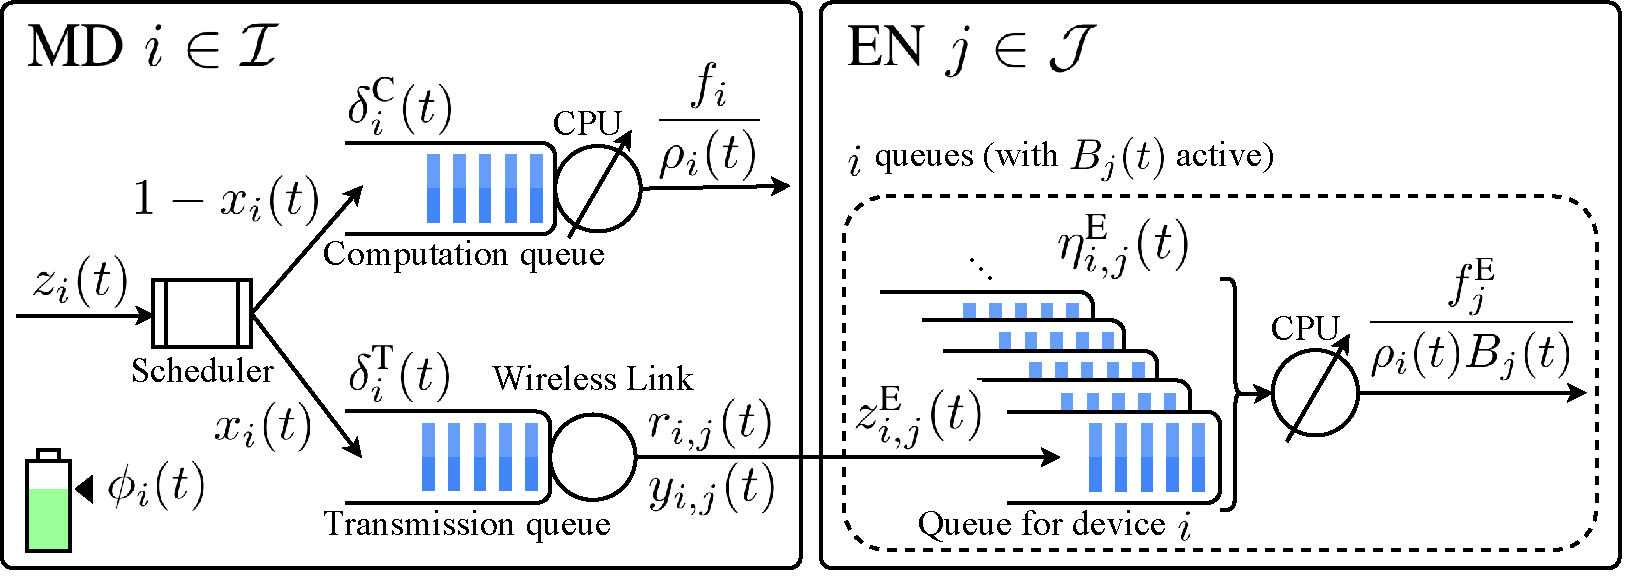
\includegraphics[width=.7\linewidth]{ queue}
	\vspace*{-1mm}
	\caption{An illustration of MD $i \in \mathcal{I}$ and EN $j \in \mathcal{J}$ in the MEC system.}
	\vspace*{-3mm}
	\label{fig1}
\end{figure}


We define $z_i(t)$ as the index assigned to the computation task arriving at MD $i \in \mathcal{I}$ in time slot $t \in \mathcal{T}$. Let $\lambda_i(t)$ denote the size of this task in bits. \textcolor{blue}{The size of task \( z_i(t) \) is selected randomly and uniformly from a discrete set \( \Lambda = \{\lambda_1, \lambda_2, \ldots, \lambda_{\theta}\} \), where \( \theta \) represents the number of these values. Note that task sizes are drawn from a discrete set since, in many applications, tasks typically come with predefined sizes,~\cite{wang2020intelligent},~\cite{zhang2019toward},~\cite{allahham2022multi}. We consider $\lambda_i(t) \in \Lambda \cup \{0\}$ to include the case that no task has arrived.} We also denote the task's processing density as $\rho_i(t)$ that indicates the number of CPU cycles required to complete the execution of a unit of the task. Furthermore, we denote the deadline of this task by $\Delta_i(t)$ which is the number of time slots that the task must be completed to avoid being dropped.

%At the beginning of time slot $t \in \mathcal{T}$, if MD $i \in \mathcal{I}$ has a newly arrived task, we define $z_i(t)$ as the unique index assigned to that task. Let $\lambda_i(t)$ be the number of newly arrived bits at the beginning of time slot $t \in \mathcal{T}$. If a new task $z_i(t)$ exists at the start of time slot $t$, then $\lambda_i(t)$ is equal to the size of task $z_i(t)$. Otherwise, $\lambda_i(t) = 0$. We consider $\rho_i(t)$ to represent the processing density of task $z_i(t)$, indicating the number of CPU cycles required to process a unit of the task.

We define two binary variables, $x_i(t)$ and $y_{i,j}(t)$ for $i \in \mathcal{I}$ and $j \in \mathcal{J}$ to determine the offloading decision and offloading target, respectively. Specifically, $x_i(t)$ indicates whether task $z_i(t)$ is assigned to the computation queue ($x_i(t) = 0$) or to the transmission queue ($x_i(t) = 1$), and $y_{i,j}(t)$ indicates whether task $z_i(t)$ is offloaded to EN $j \in \mathcal{J}$. If the task is dispatched to EN $j$, we set $y_{i,j}(t) = 1$; otherwise, $y_{i,j}(t) = 0$.





\subsection{Communication Model}
We consider that the tasks in the transmission queue are dispatched to the appropriate ENs via the MD wireless interface. We denote the transmission rate of MD $i$'s interface when communicating with EN $j \in \mathcal{J}$ in time $t$ as $r_{i,j}(t)$. In time slot $t \in \mathcal{T}$, if task $z_i(t)$ is assigned to the transmission queue for computation offloading, we define $l_i^{\text{T}}(t) \in \mathcal{T}$ to represent the time slot when the task is either dispatched to the EN or dropped. We also define $\delta_i^{\text{T}}(t)$ as the number of time slots that task $z_i(t)$ should wait in the queue before transmission. It should be noted that MD $i$ computes the value of $\delta_i^{\text{T}}(t)$ before making a decision. The value of $\delta_i^{\text{T}}(t)$ is computed as follows:
\begin{alignat}{1}
	\delta_i^{\text{T}}(t) =\textcolor{white}{i} \left[ \textcolor{white}{i}\max\limits_{t^{'}\textcolor{white}{i} \in \textcolor{white}{i} \{0,1,\ldots,t-1\}} l_i^{\text{T}}\textcolor{white}{i}(t^{'})-t+1\textcolor{white}{i}\right]^+\textcolor{white}{i},
	\label{1}  
\end{alignat}
where $[\cdot]^+ =$ max$(0, \cdot)$ and $l_i^{\text{T}}(0)=0$ for the simplicity of presentation. Note that the value of $\delta_i^{\text{T}}(t)$ only depends on $l_i^{\text{T}}(t)$ for $t' < t$. If MD $i \in \mathcal{I}$ schedules task $z_i(t)$ for dispatching in time slot $t \in \mathcal{T}$, then it will either be dispatched or dropped in time slot $l_i^{\text{T}}(t)$, which is
\begin{alignat}{1}
	l_i^{\text{T}}(t) = \min \Big\{t + \delta_i^{\text{T}}(t) + \lceil{D_i^{\text{T}}(t)}\rceil - 1, t + \Delta_i(t) - 1\Big\},
	\label{2}  
\end{alignat}
where $D_i^{\text{T}}(t)$ refers to the number of time slots required for the transmission of task $z_i(t)$ from MD $i \in \mathcal{I}$ to EN $j \in \mathcal{J}$. We have
\begin{alignat}{1}
	D_i^{\text{T}}(t) =  \sum_{\mathcal{J}} y_{i,j}(t) {\lambda_i(t) \over r_{i,j}(t)\tau}.
	\label{3}  
\end{alignat}
Let $E_i^{\text{T}}(t)$ denote the energy consumption of the transmission from MD $i \in \mathcal{I}$ to EN $j \in \mathcal{J}$. We have
\begin{alignat}{1}
	E_i^{\text{T}}(t) = D_i^{\text{T}}(t)p_i^{\text{T}}(t)\tau,
	\label{4}  
\end{alignat}
where $p_i^{\text{T}}(t)$ represents the power consumption of the communication link of MD $i \in \mathcal{I}$ in time slot $t$.
\subsection{Computation Model}
The computation tasks can be executed either locally on the MD or on the EN. In this subsection, we provide a detailed explanation of these two cases.
\subsubsection{Local Execution}
We model the local execution by a queuing system consisting the computation queue and the MD processor. Let $f_i$ denote the MD $i$'s processing power (in cycle per second). When task $z_i(t)$ is assigned to the computation queue at the beginning of time slot $t \in \mathcal{T}$, we define $l_i^{\text{C}}(t) \in \mathcal{T}$ as the time slot during which task $z_i(t)$ will either be processed or dropped. If the computation queue is empty, $l_i^{\text{C}}(t) = 0$. Let $\delta_i^{\text{C}}(t)$ denote the number of remaining time slots before processing task $z_i(t)$ in the computation queue. We have:
\begin{alignat}{1}
	\delta_i^{\text{C}}(t) = \left[ \max \limits_{t' \in \{0,1,\ldots,t-1\}} l_i^{\text{C}}(t')-t+1 \right]^+.
	\label{5}  
\end{alignat}
%In the above relation, the operator $[z]^+ = \max{0, z}$ is defined, and the variable $l_i^{\text{C}}(0) = 0$. Specifically, the expression $\max_{t' \in {0,1,2,\ldots,t-1}} l_i^{\text{C}}(t')$ determines the time slot until which all tasks placed in the local computation queue have been completed before time slot $t$. Therefore, $\delta_i^{\text{C}}(t)$ represents the number of time slots that task $z_i(t)$ needs to wait for processing. For example, suppose task $z_i(1)$ is in the computation queue, and its processing will be completed in time slot 5. Hence, $l_i^{\text{C}}(1) = 5$, meaning that the task should remain in the queue for $\Delta^{comp}(3) = [\max{5,0}-3+1]^+ = 3$ time slots until the process is finished.
In the equation above, the term $\max_{t' \in \{0, 1, \ldots, t-1\}} l_i^{\text{C}}(t')$ denotes the time slot at which each existing task in the computation queue, which arrived before time slot $t$, is either processed or dropped. Consequently, $\delta_i^{\text{C}}(t)$ denotes the number of time slots that task $z_i(t)$ should wait before being processed. We denote the time slot in which task $z_i(t)$ will be completely processed by $l_i^{\text{C}}(t)$ if it is assigned to the computation queue for local processing in time slot $t$. We have
\begin{alignat}{1}
	l_i^{\text{C}}(t) = \min \Big\{t + \delta_i^{\text{C}}(t) + \lceil D_i^{\text{C}}(t) \rceil - 1, t + \Delta_i(t) - 1\Big\}.
	\label{6}  
\end{alignat}
The task $z_i(t)$ will be immediately dropped if its processing is not completed by the end of the time slot $t + \Delta_i(t) - 1$. In addition, we introduce $D_i^{\text{C}}(t)$ as the number of time slots required to complete the processing of task $z_i(t)$ on MD $i \in \mathcal{I}$. It is given by:
\begin{alignat}{1}
	D_i^{\text{C}}(t) = { \lambda_i(t)  \over  f_i  \tau /  \rho_i(t)}.
	\label{7}  
\end{alignat}



%In particular, the processing of task $z_i(t)$ will commence at time $t + \delta_i^{\text{C}}(t)$. Therefore, the first component of the minimum operator is equal to the duration of time in which task $z_i(t)$ is completed without exceeding its deadline, denoted by $\delta_i^{\text{C}}(t)$. The second component refers to the duration of time in which task $z_i(t)$ becomes expired and discarded. As a result, $l_i^{\text{C}}(t)$ represents the time slot in which task $z_i(t)$ will be completed.
To compute the MD's energy consumption in the time slot $t \in \mathcal{T}$, we define $E_i^{\text{L}}(t)$ as:
\begin{alignat}{1}
	E_i^{\text{L}}(t) =  D_i^{\text{C}}(t) p_i^{\text{C}}  \tau, %=  { \lambda_i(t) \rho_i(t)  \over  f_i} p_i^{\text{C}},
	\label{8}  
\end{alignat}
where $p_i^{\text{C}} = 10^{-27}(f_i)^3$ represents the energy consumption of MD $i$'s CPU frequency \cite{mao2016dynamic}.
\subsubsection{Edge Execution}
We model the edge execution by the queues associated with MDs deployed at ENs. If computation task $z_i(t')$ is dispatched to EN $j$ in time $t' < t$, we let $z_{i,j}^{\text{E}}(t)$ and $\lambda_{i,j}^{\text{E}}(t)$ (in bits) denote the unique index of the task and the size of the task in the $i^{\text{th}}$ queue at EN $j$. We define $\eta_{i,j}^{\text{E}}(t)$ (in bits) as the length of this queue at the end of time slot $t \in \mathcal{T}$. We refer to a queue as an active queue in a certain time slot if it is not empty. That being said, if at least one task is already in the queue from previous time slots or there is a task arriving at the queue, that queue is active. We define $\mathcal{B}_j(t)$ to denote the set of active queues at EN $j$ in time slot $t$.
\begin{alignat}{1}
	\mathcal{B}_j(t) = \textcolor{white}{i}\Big\{i \textcolor{white}{i}\big| i \in \mathcal{I}, \lambda_{i,j}^{\text{E}}(t)>0\,\, \textcolor{white}{i}\text{or}\textcolor{white}{i} \,\, \eta_{i,j}^{\text{E}}(t-1)>0\textcolor{white}{i}\Big\}.\textcolor{white}{i}
	\label{9}  
\end{alignat}
We introduce $b_j(t) \triangleq |\mathcal{B}_j(t)|$ that represents the number of active queues in EN $j \in \mathcal{J}$ in time slot $t \in \mathcal{T}$. In each time slot $t \in \mathcal{T}$, the EN's processing power is divided among its active queues using a generalized processor sharing method~\cite{parekh1993generalized}. Let variable $f_j^{\text{E}}$ (in cycles per second) represent the computational capacity of EN $j$. Therefore, EN $j$ can allocate computational capacity of $f_j^{\text{E}}/(\rho_i(t) b_j(t))$ to each MD $i \in \mathcal{B}_j(t)$ during time slot $t$. To calculate the length of the computation queue for MD $i \in \mathcal{I}$ in EN $j \in \mathcal{J}$, we define $\omega_{i,j}(t)$ (in bits) to represent the number of bits from dropped tasks in that queue at the end of time slot $t \in \mathcal{T}$. The backlog of the queue, referred to as $\eta_{i,j}^{\text{E}}(t)$ is given by:
\begin{alignat}{1}
	\eta_{i,j}^{\text{E}}(t)\hspace{-0.8mm}=\hspace{-1mm}\left[\eta_{i,j}^{\text{E}}(t-1)\hspace{-0.6mm}+\hspace{-0.7mm}\lambda_{i,j}^{\text{E}}(t)\hspace{-0.7mm}-\hspace{-0.7mm}{f_j^{\text{E}}\tau\over \rho_i(t)b_j(t)} -\omega_{i,j}(t)\right]^+\hspace{-1mm}.
	\label{10}  
\end{alignat}
We also define $l_{i,j}^{\text{E}}(t) \in \mathcal{T}$ as the time slot during which the offloaded task $z_{i,j}^{\text{\text{E}}}(t)$ is either processed or dropped by EN $j$. Given the uncertain workload ahead at EN $j$, neither MD $i$ nor EN $j$ has information about $l_{i,j}^{\text{E}}(t)$ until the corresponding task $z_{i,j}^{\text{E}}(t)$ is either processed or dropped. Let $\hat{l}_{i,j}^{\text{E}}(t)$ represent the time slot at which the execution of task $z_{i,j}^{\text{E}}(t)$ starts. In mathematical terms, for $i \in \mathcal{I}$, $j \in \mathcal{J}$, and $t \in \mathcal{T}$, we have:
\begin{alignat}{1}
	\hat{l}_{i,j}^{\text{E}}(t) = \max \{t, \max \limits_{t^{'} \in \{0,1,\ldots,t-1\}} l_{i,j}^{\text{E}}(t^{'})+1\},
	\label{11}  
\end{alignat}
where $l_{i,j}^{\text{E}}(0) = 0$. Indeed, the initial processing time slot of task $z_{i,j}^{\text{E}}(t)$ at EN should not precede the time slot when the task was enqueued or when the previously arrived tasks were processed or dropped. Therefore, $l_{i,j}^{\text{E}}(t)$ is the time slot that satisfies the following constraints. %For $i \in \mathcal{I}$, $j \in \mathcal{J}$, and $t \in \mathcal{T}$,
\begin{alignat}{1}
	\sum_{t^{'}=\hat{l}_{i,j}^{\text{E}}(t)}^{l_{i,j}^{\text{E}}(t)}{f_j^{\text{E}}\tau \over \rho_i(t)b_j(t^{'})}\mathbbm{1}(i \in \mathcal{B}_j(t^{'}))  \geq   \lambda_{i,j}^{\text{E}}(t),
	\label{12}  \\
	\sum_{t^{'}=\hat{l}_{i,j}^{\text{E}}(t)}^{l_{i,j}^{\text{E}}(t)-1}{f_j^{\text{E}}\tau \over \rho_i(t)b_j(t^{'})}\mathbbm{1}(i \in \mathcal{B}_j(t^{'})) < \lambda_{i,j}^{\text{E}}(t),
	\label{13}  
\end{alignat}
where $\mathbbm{1} (z \in \mathbb{Z})$ is the indicator function. In particular, the total processing capacity that EN $j$ allocates to MD $i$ from the time slot $\hat{l}_{i,j}^{\text{E}}(t)$ to the time slot $l_{i,j}^{\text{E}}(t)$ should exceed the size of task $z_{i,j}^{\text{E}}(t)$. Conversely, the total allocated processing capacity from the time slot $l_{i,j}^{\text{E}}(t)$ to the time slot $l_{i,j}^{\text{E}}(t)-1$ should be less than the task's size.

Additionally, we define $D_{i,j}^{\text{E}}(t)$ to represent the quantity of processing time slots allocated to task $z_{i,j}^{\text{E}}(t)$ when executed at EN $j$. This value is given by:
\begin{alignat}{1}
	D_{i,j}^{\text{E}}(t) = { \lambda_{i,j}^{\text{E}}(t) \rho_i(t) \over f_j^{\text{E}} \tau /  b_j(t)}.
	\label{14}  
\end{alignat}
We also define $E_{i,j}^{\text{E}}(t)$ as the energy consumption of processing at EN $j$ in time slot $t$ by MD $i$. This can be calculated as:
\begin{alignat}{1}
	E_{i,j}^{\text{E}}(t) = {D_{i,j}^{\text{E}}(t)  p_j^{\text{E}} \tau \over b_j(t)},  % = { \lambda_{i,j}^{\text{E}}(t) \rho_i(t) \over  f_j^{\text{E}}}p_j^{\text{E}} ,
	\label{15}  
\end{alignat}
where $p_j^{\text{E}}$ is a constant value which denotes the energy consumption of the EN $j$'s processor when operating at full capacity. 

In addition to the energy consumed by EN $j$ for task processing, we also take into account the energy consumed by the MD $i$'s user interface in the standby state while waiting for task completion at the EN $j$. We define $E_{i,j}^{\text{I}}(t)$ as the energy consumption associated with the user interface of MD $i \in \mathcal{I}$, which is given by
\begin{alignat}{1}
	E_i^{\text{I}}(t) = D_{i,j}^{\text{E}}(t) p_i^{\text{I}} \tau, %= {\lambda_{i,j}^{\text{E}}(t) \rho_i(t) \over \mathcal{B}_j(t) f_j^{\text{E}}} p_i^{\text{I}},
	\label{16}
\end{alignat}
where $p_i^{\text{I}}$ is the standby energy consumption of MD $i \in \mathcal{I}$.
\begin{alignat}{1}
	E_i^{\text{O}}(t) = E_i^{\text{T}}(t) + \sum_{\mathcal{J}} E_{i,j}^{\text{E}}(t) + E_i^{\text{I}}(t).
	\label{17}
\end{alignat}



\section{Task Offloading problem Formulation}
\label{section:III}

Based on the introduced system model, we present the computation task offloading problem in this section. Our primary goal is to enhance each MD's QoE individually by taking the dynamic demands of MDs into account. To achieve this, we approach the optimization problem as an MDP, aiming to maximize the MD's QoE by striking a balance among key QoE factors, including task completion, task delay, and energy consumption. To prioritize QoE factors, we utilize the MD's battery level, which plays a crucial role in decision-making. Specifically, when an MD observes its state (e.g. task size, queue details, and battery level) and encounters a newly arrived task, it selects an appropriate action for that task. The selected action, based on the observed state, will result in enhanced QoE. Each MD strives to maximize its long-term QoE by optimizing the policy mapping from states to actions. In what follows, we first present the state space, action space, and QoE function, respectively. We then formulate the QoE maximization problem for each MD.




\subsection{State Space}
A state in our MDP represents a conceptual space that comprehensively describes the state of an MD facing the environment. We represent the MD $i$'s state in time slot $t$ as vector $\boldsymbol{s}_i(t)$ that includes the newly arrived task size, the queues information, the MD's battery level, and the workload history at the ENs. The MD observers this vector at the beginning of each time slot. The vector $\boldsymbol{s}_i(t)$ is defined as follows:
\begin{alignat}{1}
	\boldsymbol{s}_i(t) = \Big(\lambda_i(t), \delta_i^{\text{C}}(t), \delta_i^{\text{T}}(t), \boldsymbol{\eta}_i^{\text{E}}\hspace{-0.4mm}(\hspace{-0.4mm}t\hspace{-0.4mm}-\hspace{-0.4mm}1\hspace{-0.5mm}),\phi_i(t), \mathcal{H}(t) \Big),
	\label{18}
\end{alignat}
where vector $\boldsymbol{\eta}_i^{\text{E}}(t-1) = (\eta_{i,j}^{\text{E}}(t-1))_{j \in \mathcal{J}}$ represents the queues length of MD $i$ in ENs at the previous time slot and is computed by the MD according to \eqref{10}. Let $\phi_i(t)$ denote the battery level of MD $i$ in time slot $t$. Considering the power modes of a real mobile device, $\phi_i(t)$ is derived from the discrete set $\Phi=\{\phi_1,\phi_2,\phi_3\}$, corresponding to ultra power-saving, power-saving, and performance modes, respectively.

In addition, to predict future EN workloads, we define the matrix $\mathcal{H}(t)$ as historical data, indicating the number of active queues for all ENs. This data is recorded over $T^{\text{s}}$ time slots, ranging from $t\hspace{-0.4mm}-\hspace{-0.4mm}T^{\text{s}}$ to $t\hspace{-0.4mm}-\hspace{-0.4mm}1$, in $T^{\text{s}}\hspace{-0.4mm}\times \hspace{-0.4mm} J$ matrix. For EN $j$ workload history at $i^{th}$ time slot from $T^{\text{s}}-t$, we define $h_{i,j}(t)$ as:
\begin{alignat}{1}
	h_{i,j}(t) = b_j(t - T^{\text{s}} + i - 1).
	\label{19}
\end{alignat}
%where $b_j(t - T^{\text{s}} + i - 1)$ is the number of active queues of EN $j$ in time slot $t - T^{\text{s}} + i - 1$. 
EN $j \in \mathcal{J}$ broadcasts $b_j(t)$ at the end of each time slot. %Given $b_j(t) \leq I$, can be represented using only a few bits, the broadcast incurs minimal signaling overhead.

We define vector $\mathcal{S}$ as the discrete and finite state space for each MD. The size of the set $\mathcal{S}$ is given by $\Lambda \times T^2 \times \mathcal{U} \times 3 \times I^{T^{\text{s}} \times J}$, where $\mathcal{U}$ is the set of available queue length values at an EN over $T$ time slots. 



%A MD $i \in \mathcal{I}$ can obtain state information $\lambda_i(t)$, $\delta_i^{\text{C}}(t)$, $\delta_i^{\text{T}}(t)$, and $\phi_i(t)$ through local observation at the beginning of time slot $t$.


%For state information  $\boldsymbol{\eta}_i^{\text{E}}(t-1)$, MD $i$ can compute this vector according to the number of transmitted bits to each EN in each time slot and the number of bits of MD $i$ processed or being dropped by each EN in each time slot according to \eqref{10}. 


%For matrix $\mathcal{H}(t)$, we assume that each EN will broadcast its number of active queues at the end of each time slot. Since the number of active queues is always a small number, which can be represented by several bits, the broadcasting will only incur a small signaling overhead.

\subsection{Action Space}
The action space represents the agent's behavior and the decisions. In this context, we define $\boldsymbol{a}_i(t)$ to denote the action taken by MD $i \in \mathcal{I}$ in time slot $t \in \mathcal{T}$. These actions involve two decisions, (a) Offloading decision to determine whether or not to offload the task, and (b) Offloading target to determine the EN to send the offloaded tasks. Thus, the action of MD $i$ in time slot $t$ can be concisely expressed as the following action tuple: \vspace{-1.5mm}
\begin{alignat}{1}
	\boldsymbol{a}_i(t) = (x_i(t), \boldsymbol{y}_i(t)),
	\label{20}
\end{alignat}
where vector $\boldsymbol{y}_i(t)=(y_{i,j}(t))_{j \in \mathcal{J}}$ represents the selected EN for offloading this task. In Section~\ref{section:1}, we will discuss about the size of this action space.

%Hence, the decision space of each MD is thus equal to $\mathcal{A} = \{0,1\}^{1+N}$, with $j$ representing the number of available ENs.




\subsection{QoE Function}
\textcolor{blue}{The QoE function evaluates the influence of agent's actions based on its personalized QoE requirement \cite{wang2017qoe}, by taking several key performance factors into account. It incorporates a multi-dimensional and adaptive structure that establishes an appropriate balance among these QoE factors according to the MD's preference, such as individual preferences for reducing task delays or energy consumption, which may vary over time \cite{wang2019intelligent}, \cite{mehrabi2019energy}. To reflect the agent’s personalized QoE requirements, an adaptive trade-off between task completion and cost reduction is designed, where a weighted sum between completion delay and energy consumption plays as an associated cost. The MDs adjusted the weights dynamically to define the significance of each factor based on its energy mode—performance, power-saving, or ultra-power-saving. 
	Based on the system model, we first calculate task delay and energy consumption and then represent the associated cost and QoE function accordingly.}

Given the selected action $\boldsymbol{a}_i(t)$ in the observed state $\boldsymbol{s}_i(t)$, we represent $\mathcal{D}_i(\boldsymbol{s}_i(t), \boldsymbol{a}_i(t))$ as the delay of task $z_i(t),$ which indicates the number of time slots from time slot $t$ to the time slot in which task $z_i(t)$ is processed. It is calculated by: \vspace{2mm}

$\mathcal{D}_i(\boldsymbol{s}_i(t),\boldsymbol{a}_i(t)) = (1-x_i(t))\Big(l_i^{\text{C}}(t) - t + 1\Big)  +  x_i(t)$
\begin{alignat}{1}
	\;\;\;\,\bigg( \sum\limits_{\mathcal{J}} \sum\limits_{t'=t}^{T} \mathbbm{1}\big(z_{i,j}^{\text{E}}(t') = z_i(t)\big) \textcolor{blue}{y_{i,j}(t)} \, l_{i,j}^{\text{E}}(t') - t +1\bigg),
	\label{21}  
\end{alignat} 
where $\mathcal{D}_i(\boldsymbol{s}_i(t),\boldsymbol{a}_i(t))= 0$ if task $z_i(t)$ is dropped. Correspondingly, we denote the energy consumption of task $z_i(t)$ when taking action $\boldsymbol{a}_i(t)$ in the observed state $\boldsymbol{s}_i(t)$ as $\mathcal{E}_i(\boldsymbol{s}_i(t),\boldsymbol{a}_i(t))$, which is: \vspace{1.7mm}


$\mathcal{E}_i(\boldsymbol{s}_i(t),\boldsymbol{a}_i(t)) = (1-x_i(t)) E_i^{\text{L}}(t)+$
\begin{alignat}{1}
	\hspace{0.9cm} x_i(t)\bigg( \sum\limits_{\mathcal{J}} \sum\limits_{t^{'}=t}^{T}\mathbbm{1}\big(z_{i,j}^{\text{E}}(t') = z_i(t)\big) \textcolor{blue}{y_{i,j}(t)}  E_i^{\text{O}}(t)  \bigg).
	\label{22}  
\end{alignat}

\textcolor{blue}{To define associated cost, we use a weighted sum between task delay $\mathcal{D}_i(\boldsymbol{s}_i(t),\boldsymbol{a}_i(t))$ and energy consumption $\mathcal{E}_i(\boldsymbol{s}_i(t),\boldsymbol{a}_i(t))$, where the weights adjust dynamically depending on the MD's energy levels to reflect the MD's preference for each factor.}
Given the delay and energy consumtion of task $z_i(t)$, we also define $\mathcal{C}_i(\boldsymbol{s}_i(t),\boldsymbol{a}_i(t))$ that denotes the assosiate cost of task $z_i(t)$ given the action $\boldsymbol{a}_i(t)$ in the state $\boldsymbol{s}_i(t)$. \vspace{1.7mm}


$\mathcal{C}_i(\boldsymbol{s}_i(t),\boldsymbol{a}_i(t)) =$
\begin{alignat}{1}
	\phi_i(t) \, \mathcal{D}_i(\boldsymbol{s}_i(t),\boldsymbol{a}_i(t)) +(1-\phi_i(t)) \, \mathcal{E}_i(\boldsymbol{s}_i(t),\boldsymbol{a}_i(t)),
	\label{23}  
\end{alignat}
where $\phi_i(t)$ represents the MD $i$'s \textcolor{blue}{energy level}. When the MD is operating in performance mode, the primary focus is on minimizing task delays, thus the delay contributes more to the cost. On the other hand, when the MD switches to ultra power-saving mode, the main attention is directed toward reducing power consumption.

Finally, we define $\boldsymbol{q}_i(\boldsymbol{s}_i(t),\boldsymbol{a}_i(t))$ as the QoE associated with task $z_i(t)$ given the selected action $\boldsymbol{a}_i(t)$ and the observed state $\boldsymbol{s}_i(t)$. The QoE function is defined as follows:\vspace{1.7mm}

$\boldsymbol{q}_i(\boldsymbol{s}_i(t),\boldsymbol{a}_i(t)) =$
\begin{alignat}{1}
	\hspace*{8mm}
	\begin{cases} 
		\mathcal{R} - \mathcal{C}_i(\boldsymbol{s}_i(t),\boldsymbol{a}_i(t)) & \hspace*{-2mm} \text{if task $z_i(t)$ is processed,} \\
		- \hspace*{0.8mm} \mathcal{E}_i(\boldsymbol{s}_i(t),\boldsymbol{a}_i(t)) &	\hspace*{-2mm} \text{if task $z_i(t)$ is dropped,}
	\end{cases}
	\label{26}  
\end{alignat}
where $\mathcal{R} > 0$ represents a constant reward for task completion. If $z_i(t) = 0$, then $\boldsymbol{q}_i(\boldsymbol{s}_i(t), \boldsymbol{a}_i(t)) = 0$. Throughout the rest of this paper, we adopt the shortened notation $\boldsymbol{q}_i(t)$ to represent $\boldsymbol{q}_i(\boldsymbol{s}_i(t), \boldsymbol{a}_i(t))$.






\subsection{Problem Formulation}
We define the task offloading policy for MD $i \in \mathcal{I}$ as a mapping from its state to its corresponding action, denoted by i.e., $\pi_i : \mathcal{S} \rightarrow \mathcal{A}$. Especially, MD $i$ determines an action $\boldsymbol{a}_i(t) \in \mathcal{A}$, according to policy $\pi_i$ given the observed environment state $\boldsymbol{s}_i(t) \in \mathcal{S}$. The MD aims to find its optimal policy $\pi_i^*$ which maximizes the long-term QoE,
\begin{alignat}{1}
	\pi_i^* = \text{arg}\,\,  \max\limits_{\pi_i}  \mathbbm{E} \Bigg[ \sum\limits_{t \in \mathcal{T}}  \gamma^{t-1}\boldsymbol{q}_i(t) \Bigg| \pi_i \Bigg],
	\label{24}  
\end{alignat}
where $\gamma \in (0,1]$ is a discount factor and determines the balance between instant QoE and long-term QoE. As $\gamma$ approaches 0, the MD prioritizes QoE within the current time slot exclusively. Conversely, as $\gamma$ approaches 1, the MD increasingly factors in the cumulative long-term QoE. The expectation $\mathbb{E}[\cdot]$ is taken into consideration of the time-varying system environments. Solving the optimization problem in \eqref{24} is particularly challenging due to the dynamic nature of the network. To address this challenge, we introduce a DRL- based offloading algorithm to learn the mapping between each state-action pair and their long-term QoE.
\section{DRL-Based Offloading Algorithm} \label{section:V}
We now present QECO algorithm so as to address the distributed offloading decision-making of MDs. The aim is to empower MDs to identify the most efficient action that maximizes their long-term QoE. In the following, we introduce a neural network that characterizes the MD's state-action Q-values mapping, followed by a description of the information exchange between the MDs and ENs.




\subsection{DQN-based Approach}
We utilize the DQN technique to find the mapping between each state-action pair to Q-values in the formulated MDP. As shown in Fig.~\ref{DQN}, each MD $i \in \mathcal{I}$ is equipped with a neural network comprising six layers. These layers include an input layer, an LSTM layer, two dense layers, an advantage-value (A\&V) layer, and an output layer. The parameter vector $\theta_i$ of MD $i$'s neural network is defined to maintain the connection weights and neuron biases across all layers. For MD $i \in \mathcal{I}$, we utilize the state information as the input of neural network. The state information $\lambda_i(t)$, $\delta_i^{\text{C}}(t)$, $\delta_i^{\text{T}}(t)$, $\phi_i(t)$, and $\boldsymbol{\eta}_i^{\text{E}}(t-1)$ are directly passed to the dense layer, while the state information $\mathcal{H}(t)$ is first supplied to the LSTM layer and then the resulting output is sent to the dense layer. The role and responsibilities of each layer are detailed as follows.


\subsubsection{Predicting Workloads at ENs}
In order to capture the dynamic behavior of workloads at the ENs, we employ the LSTM network \cite{hochreiter1997long}. This network maintains a memory state $\mathcal{H}(t)$ that evolves over time, enabling the neural network to predict future workloads at the ENs based on historical data. By taking the matrix $\mathcal{H}(t)$ as an input, the LSTM network learns the patterns of workload dynamics. The architecture of the LSTM consists of $T^{\text{s}}$ units, each equipped with a set of hidden neurons, and it processes individual rows of the matrix $\mathcal{H}(t)$ sequentially. Through this interconnected design, MD tracks the variations in sequences from $\boldsymbol{h}_1(t)$ to $\boldsymbol{h}_{T^{\text{s}}}(t)$, where vector $\boldsymbol{h}_i(t) = (h_{i,j}(t))_{j \in \mathcal{J}}$, thereby revealing workload fluctuations at the ENs across different time slots. The final LSTM unit produces an output that encapsulates the anticipated workload dynamics, and is then connected to the subsequent layer neurons for further learning.




%\subsubsection{workload Prediction}
%To learning the dynamics of the workloads at the ENs, we use the LSTM network [26], [27], which can keep track of the state $\mathcal{H}(t)$ over time. It can provide the neural network the ability of estimating the workloads at the ENs in the future using the history. The LSTM network takes the matrix $\mathcal{H}(t)$ as input so as to learn the workload dynamics. coresponding the matrix $\mathcal{H}(t)$,  The LSTM network contains $T^{\text{s}}$ LSTM units, each of which contains a set of hidden neurons and takes one row of the matrix $\mathcal{H}(t)$ as input. These LSTM units are connected in sequence so as to keep track of the variations of the sequences from $\{\mathcal{H}(t)\}_1$ to $\{\mathcal{H}(t)\}_{T^{\text{s}}}$, which can reveal the variations of the workloads at the ENs among time slots. The LSTM network will output the information that indicates the dynamics of the workloads in the future in the last LSTM unit, where the output will be connected to the neurons in the next layer for further learning.
%
%---------------------

%This layer is responsible for learning the dynamics of the workloads at the ENs. This is achieved by including an LSTM network [26], [27]. We use the LSTM network because it can keep track of the state $\textbf{H}(t)$ over time. It can provide the neural network the ability of estimating the workloads at the ENs in the future using the history. 
%
%Specifically, the LSTM network takes the matrix $\textbf{H}(t)$ as input so as to learn the workload dynamics. Fig. 3 shows the structure of an LSTM network. The LSTM network contains Tstep LSTM units, each of which contains a set of hidden neurons. Each LSTM unit takes one row of the matrix $\textbf{H}(t)$ as input, we let $\{\textbf{H}(t)\}_1$  denote the $i^{th}$ row of matrix $\textbf{H}(t)$ in Fig. 3. These LSTM units are connected in sequence so as to keep track of the variations of the sequences from $\{\textbf{H}(t)\}_1$ to $\{\textbf{H}(t)\}_{T^{step}}$, which can reveal the variations of the workloads at the ENs among time slots. The LSTM network will output the information that indicates the dynamics of the workloads in the future in the last LSTM unit, where the output will be connected to the neurons in the next layer for further learning.



\subsubsection{State-Action Q-Value Mapping}
The pair of dual dense layers plays a crucial role in learning the mapping of Q-values from the current state and the learned load dynamics to the corresponding actions. The dense layers consist of a cluster of neurons that employ rectified linear units (ReLUs) as their activation functions. In the initial dense layer, connections are established from the neurons in the input layer and the LSTM layer to each neuron in the dense layer. The resulting output of a neuron in the dense layer is connected to each neuron in the subsequent dense layer. In the second layer, the outputs from each neuron establish connections with all neurons in the A\&V layers.



\subsubsection{Dueling-DQN Approach for Q-Value Estimation}
In the neural network architecture, the A\&V layer and the output layer incorporate the principles of the dueling-DQN \cite{wang2016dueling} to compute action Q-values. The fundamental concept of dueling-DQN involves two separate learning components: one for action-advantage values and another for state-value. This approach enhances Q-value estimation by separately evaluating the long-term QoE attributed to states and actions.



The A\&V layer consists of two distinct dense networks referred to as network A and network V. Network A's role is to learn the action-advantage value for each action, while network V focuses on learning the state-value. For an MD $i \in \mathcal{I}$, we define $V_i(\boldsymbol{s}_i(t); \theta_i)$ and $A_i(\boldsymbol{s}_i(t), \boldsymbol{a}; \theta_i)$ to denote the state-value and the action-advantage value of action $\boldsymbol{a} \in \mathcal{A}$ under state $\boldsymbol{s}_i(t) \in \mathcal{S}$, respectively. The parameter $\theta_i$ is responsible for determining these values, and it can be adjusted when training the QECO algorithm.

For an MD $i \in \mathcal{I}$, the A\&V layer and the output layer collectively determine $Q_i(\boldsymbol{s}_i(t), \boldsymbol{a}; \theta_i)$, representing the resulting Q-value under action $\boldsymbol{a} \in \mathcal{A}$ and state $\boldsymbol{s}_i(t) \in \mathcal{S}$, as follows: \vspace{1.7mm}


$Q_i(\boldsymbol{s}_i(t), \boldsymbol{a}; \theta_i) = V_i(\boldsymbol{s}_i(t);\theta_i) +$
\begin{alignat}{1}
	\hspace{0.94cm} \Bigg( A_i(\boldsymbol{s}_i(t),\boldsymbol{a};\theta_i) - {1 \over |\mathcal{A}|} \sum\limits_{\boldsymbol{a}' \in \mathcal{A}}(A_i(\boldsymbol{s}_i(t),\boldsymbol{a}';\theta_i) \Bigg),
	\label{25}  
\end{alignat}
where $\theta_i$ establishes a functional relationship that maps Q-values to pairs of state-action.

%, which characterizes the long-term QoE under any observed state $\boldsymbol{s}_i(t) \in \mathcal{S}$ and action $\mathcal{A} \in \mathcal{A}$. 




\subsection{QoE-Oriented DRL-Based Algorithm}
\label{section:1}

%Our proposed QoE-Driven DRL-Based Algorithm is designed to efficiently distribute computational loads for training neural networks on MDs while leveraging the support of ENs. The primary objective of this algorithm is to utilize the experience of each MD to train its neural network, allowing the MD to make informed decisions that maximize its long-term QoE. To achieve efficient training, each MD $i \in \mathcal{I}$ is paired with a dedicated EN $n_i \in \mathcal{J}$ that assists in the training process. The selection of EN $n_i$ is based on its maximum transmission capacity with MD $i$. We define the set $\mathcal{I}_j \subset \mathcal{I}$ as the group of MDs whose training is facilitated by EN $j \in \mathcal{J}$.

The QECO algorithm is meticulously designed to optimize the allocation of computational tasks between MDs and ENs. Since the training of neural networks imposes an extensive computational workload on MDs, we enable MDs to utilize ENs for training their neural networks, effectively reducing their computational workload. For each MD $i \in \mathcal{I}$, there is an associated EN, denoted as EN $j_i \in \mathcal{J}$, which assists in the training process. This EN possesses the highest transmission capacity among all ENs. We define $\mathcal{I}_j \subset \mathcal{I}$ as the set of MDs for which training is executed by EN $j \in \mathcal{J}$, i.e. $\mathcal{I}_j = \{i \in \mathcal{I} | j_i = j\}$. This approach is feasible due to the minimal information exchange and processing requirements for training compared to MD's tasks. The algorithms to be executed at MD $i \in \mathcal{I}$ and EN $j \in \mathcal{J}$ are given in Algorithms ~\ref{alg:cap} and ~\ref{alg:cap2}, respectively. The core concept involves training neural networks with MD experiences (i.e., state, action, QoE, next state) to map Q-values to each state-action pair. This mapping allows MD to identify the action in the observed state with the highest Q-value and maximize its long-term QoE.




In detail, EN $j \in \mathcal{J}$ maintains a replay buffer denotes as $\mathcal{M}_i$ with two neural networks for MD $i$: $\textit{Net}_i^{\text{E}}$, denoting the evaluation network, and $\textit{Net}_i^{\text{T}}$, denoting the target network, which have the same neural network architecture. However, they possess distinct parameter vectors $\theta^{\text{E}}_i$ and $\theta^{\text{T}}_i$, respectively. Their Q-values are represented by $Q_i^{\text{E}}(\boldsymbol{s}_i(t), \boldsymbol{a}; \theta^{\text{E}}_i)$ and $Q_i^{\text{T}}(\boldsymbol{s}_i(t), \boldsymbol{a}; \theta^{\text{T}}_i)$ for MD $i \in \mathcal{I}_j$, respectively, associating the action $\boldsymbol{a} \in \mathcal{A}$ under the state $\boldsymbol{s}_i(t) \in \mathcal{S}$. The replay buffer records the observed experience $(\boldsymbol{s}_i(t), \boldsymbol{a}_i(t), \boldsymbol{q}_i(t), \boldsymbol{s}_i(t+1))$ of MD $i$. Moreover, $\textit{Net}_i^{\text{E}}$ is responsible for action selection, while $\textit{Net}_i^{\text{T}}$ characterizes the target Q-values, which represent the estimated long-term QoE resulting from an action in the observed state. The target Q-value serves as the reference for updating the network parameter vector $\theta^{\text{E}}_i$. This update occurs through the minimization of disparities between the Q-values under $\textit{Net}_i^{\text{E}}$ and $\textit{Net}_i^{\text{T}}$. In the following, we introduce the offloading decision algorithm of MD $i \in \mathcal{I}$ and the training process algorithm running in EN $j \in \mathcal{J}$.

% i.e., $\textbf{\textit{s}}_i(1) = \big(\lambda_i(1), \delta_i^{\text{C}}(1), \delta_i^{\text{T}}(1), \boldsymbol{\eta}_i^{\text{E}}(0),\phi_i(1), \mathcal{H}(1) \big)$, where we set $\boldsymbol{\eta}_i^{\text{E}}(0)=0$ for all $j \in \mathcal{J}$, and $ \mathcal{H}(1)$ is a zero matrix with size $T^s \times N$. 




\subsubsection{Offloading Decision Algorithm at MD $i \in \mathcal{I}$}
We analyze a series of episodes, where $N^{\text{ep}}$ denotes the number of them. At the beginning of each episode, if MD $i \in \mathcal{I}$ receives a new task $z_i(t)$, it initializes the state $\mathcal{S}_i(1)$ and sends an $\textit{UpdateRequest}$ to EN $j_i$. After receiving the requested vector $\theta_i^{\text{E}}$ of $\textit{Net}_i^{\text{E}}$ from EN $j_i$, MD $i$ chooses the following action for task $z_i(t)$.
\begin{alignat}{1}
	\hspace*{-2mm}\boldsymbol{a}_i(t) \hspace*{-0.5mm} = \hspace*{-0.5mm}
	\begin{cases} 
		\text{arg $\max_{\boldsymbol{a}\in \mathcal{A}}Q_i^{\text{E}}(\boldsymbol{s}_i(t), \boldsymbol{a}; \theta^{\text{E}}_i)$,} & \text{w.p. $1-\boldsymbol{\epsilon}$,} \\
		\text{pick a random action from $\mathcal{A}$,} & \text{w.p. $\boldsymbol{\epsilon}$,}
	\end{cases}
	\label{26}  
\end{alignat}
where w.p. stands for with probability, and $\boldsymbol{\epsilon}$ represents the random exploration probability. The value of $Q_i^{\text{E}}(\boldsymbol{s}_i(t), \boldsymbol{a}; \theta^{\text{E}}_i)$ indicates the Q-value under the parameter $\theta^{\text{E}}_i$ of the neural network $\textit{Net}_i^{\text{E}}$. Specifically, the MD with a probability of $1 - \boldsymbol{\epsilon}$ selects the action associated with the highest Q-value under $\textit{Net}_i^{\text{E}}$ in the observed state $\boldsymbol{s}_i(t)$.


In the next time slot $t+1$, MD $i$ observes the state $\mathcal{S}_i(t+1)$. However, due to the potential for tasks to extend across multiple time slots, QoE $\boldsymbol{q}_i(t)$ associated with task $z_i(t)$ may not be observable in time slot $t+1$. On the other hand, MD $i$ may observe a group of QoEs associated with some tasks $z_i(t')$ in time slots $t' \leq t$. For each MD $i$, we define the set $\mathcal{F}_i^t \subset \mathcal{T}$ to denote the time slots during which each arriving task $z_i(t')$ is either processed or dropped in time slot $t$, as given by: \vspace{2mm}

$\mathcal{F}_i^t =\bigg \{ t' \bigg|\; t' \leq t,\; \lambda_i(t')>0, \; (1 - x_i(t')) \; l_i^{\text{C}}(t') \; + $ \vspace{-3mm}
\begin{equation}
	\hspace{10mm} x_i(t')\sum\limits_{\mathcal{J}} \sum\limits_{n= t'}^{t}\mathbbm{1}(z_{i,j}^{\text{E}}(n)=z_i(t'))  \; \textcolor{blue}{y_{i,j}(x)} \, l_{i,j}^{\text{E}}(n) = t \bigg\}.
	\label{27}  
	\nonumber
\end{equation}
Therefore, MD $i$ observes a set of QoEs $\{\boldsymbol{q}_i(t') \mid t' \in \mathcal{F}_i^t\}$ at the beginning of time slot $t+1$, where the set $\mathcal{F}_i^t$ for some $i \in \mathcal{I}$ can be empty. Subsequently, MD $i$ sends its experience $(\boldsymbol{s}_i(t), \boldsymbol{a}_i(t), \boldsymbol{q}_i(t), \boldsymbol{s}_i(t+1))$ to EN $j_i$ for each task $z_i(t')$ in $t' \in \mathcal{F}_i^t$.



\subsubsection{Training Process Algorithm at EN $j \in \mathcal{J}$}
Upon initializing the replay buffer $\mathcal{M}_i$ with the neural networks $\textit{Net}_i^{\text{E}}$ and $\textit{Net}_i^{\text{T}}$ for each MD $i \in \mathcal{I}_j$, EN $j \in \mathcal{J}$ waits for messages from the MDs in the set $\mathcal{I}_j$. When EN $j$ receives an $\textit{UpdateRequest}$ signal from an MD $i \in \mathcal{I}_j$, it responds by transmitting the updated parameter vector $\theta^{\text{E}}_i$, obtained from $\textit{Net}_i^{\text{E}}$, back to MD $i$. On the other side, if EN $j$ receives an experience $(\boldsymbol{s}_i(t), \boldsymbol{a}_i(t), \boldsymbol{q}_i(t), \boldsymbol{s}_i(t+1))$ from MD $i \in \mathcal{I}_j$, the EN stores this experience in the replay buffer $\mathcal{M}_i$ associated with that MD. %The replay buffer operates at maximum capacity and FIFO principle.

The EN randomly selects a sample collection of experiences from the replay buffer, denoted as $\mathcal{N}$. For each experience $n \in \mathcal{N}$, it calculates the value of $	\hat{Q}^{\text{T}}_{i,n}$. This value represents the QoE in experience $n$ and includes a discounted Q-value of the action anticipated to be taken in the subsequent state of experience $n$, according to the network $\textit{Net}^\text{T}_i$, given by
\begin{alignat}{1}
	\hat{Q}_{i,n}^{\text{T}} = \boldsymbol{q}_i(n) + \gamma Q_i^{\text{T}}(\boldsymbol{s}_i(n+1)), \tilde{\boldsymbol{a}}_n; \theta_i^{\text{T}}),
	\label{28}  
\end{alignat}  
where $\tilde{\boldsymbol{a}}_n$ denotes the optimal action for the state $\boldsymbol{s}_i(n+1)$ based on its highest Q-value under $\textit{Net}_i^{\text{E}}$, as given by:
\begin{alignat}{1}
	\tilde{\boldsymbol{a}}_n = \text{arg} \; \max_{\boldsymbol{a} \in \mathcal{A}} \; Q_i^{\text{E}}(\boldsymbol{s}_i(n+1), \boldsymbol{a}; \theta_i^{\text{E}}).
	\label{29}  
\end{alignat} 
In particular, regarding experience $n$, the target-Q value $\hat{Q}_{i,n}^{\text{T}}$ represents the long-term QoE for action $\boldsymbol{a}_i(n)$ under state $\boldsymbol{s}_i(n)$. This value corresponds to the QoE observed in experience $n$, as well as the approximate expected upcoming QoE. %based on $\textit{Net}_i^{\text{T}}_i$, i.e., $\gamma Q_i^{\text{T}}(\mathcal{S}_i(i+1)), \mathcal{A}_i^{\text{N}}; \theta_i^{\text{T}})$
%Based on the set $\mathcal{N}$, the EN trains the MD's neural network using previous sample experiences. Simultaneously, it updates $\theta^{\text{E}}_i$ in $\textit{Net}_i^{\text{E}}$ and computes vector $\hat{\mathbf{Q}}_i^{\text{T}} = (\hat{Q}^{\text{T}}_{i,n})_{n \in \mathcal{N}}$. The key idea of updating $\textit{Net}_i^{\text{E}}$ is to minimize the disparity in Q-values between $\textit{Net}_i^{\text{E}}$ and $\textit{Net}_i^{\text{T}}$, as indicated by the following loss function:
\textcolor{blue}{Based on the previous sample experiences $\mathcal{N}$, the EN computes the vector $\hat{\mathbf{Q}}_i^{\text{T}} = (\hat{Q}^{\text{T}}_{i,n})_{n \in \mathcal{N}}$ and trains the MD's neural network (in steps 11-21 of Algorithm ~\ref{alg:cap2}) to keep parameter vector $\theta^{\text{E}}_i$ in $\textit{Net}_i^{\text{E}}$ update for the MD's \textit{UpdateRequest}}. The key idea of updating $\textit{Net}_i^{\text{E}}$ is to minimize the disparity in Q-values between $\textit{Net}_i^{\text{E}}$ and $\textit{Net}_i^{\text{T}}$, as indicated by the following loss function:


\begin{alignat}{1}
	\hspace{-2mm}L(\theta_i^{\text{E}},\hat{\mathbf{Q}}_i^{\text{T}}) = {1 \over |\mathcal{N}| }\hspace{-1mm} \sum\limits_{n \in \mathcal{N}} \bigg(Q_i^{\text{E}}(\boldsymbol{s}_i(n) , \boldsymbol{a}_i(n); \theta_i^{\text{E}} ) -   \hat{Q}^{\text{T}}_{i,n}  \bigg)^2.
	\label{30}  
\end{alignat}  
In every \textit{ReplaceThreshold} iterations, the update of $\textit{Net}_i^{\text{T}}$ will involve duplicating the parameters from $\textit{Net}_i^{\text{E}}$ ($\theta_i^{T} = \theta_i^{E}$). The objective is to consistently update the network parameter $\theta_i^{T}$ in $\textit{Net}_i^{\text{T}}$, which enhances the approximation of the long-term QoE when computing the target Q-values in \eqref{28}.\\

\subsubsection{Computational Complexity}


The computational complexity of the QECO algorithm is determined by the number of experiences required to discover the optimal offloading policy. Each experience involves backpropagation for training, which has a computational complexity of $\mathcal{O}(C)$, where $C$ represents the number of multiplication operations in the neural network. During each training round triggered by the arrival of a new task, a sample collection of experiences of size $|\mathcal{N}|$ is utilized from the replay buffer. Since the training process encompasses $N^{\text{ep}}$ episodes and there are $K$ expected tasks in each episode, the computational complexity of the proposed algorithm is $\mathcal{O}(N^{\text{ep}}K|\mathcal{N}|C$), which is polynomial. Given the integration of neural networks for function approximation, the convergence guarantee of the DRL algorithm remains an open problem. In this work, we will empirically evaluate the convergence of the proposed algorithm in Section \ref{section:2}.

%Regarding the convergence, as mentioned in many existing works (e.g., [29]), the convergence guarantee of a DRL algorithm is still an open problem. Despite the fact that the convergence of a reinforcement learning algorithm can be proven, a DRL algorithm requires function approximation (e.g., the approximation of the Q-values in deep Q-learning algorithm) using neural networks, under which the convergence may no longer be guaranteed. In this work, we empirically evaluate the convergence performance of the proposed algorithm in Section 5.1.



\section{Performance Evaluation}\label{section:VI}
In this section, we first present the simulation setup and training configuration. \textcolor{blue}{We then illustrate the convergence of the proposed DRL-based QECO algorithm under different optimization methods and hyperparameters, and evaluate its performance in comparison to three baseline schemes in addition to the existing work~\cite{qiu2020distributed}.}

%We begin by presenting the simulation setting and training configuration, followed by the evaluation of QECO algorithm under multiple key performance metrics in comparison to benchmark methods.



\subsection{Simulation Setup}
We consider a MEC environment with 50 MDs and 5 ENs, similar to \cite{9253665}. We also follow the model presented in \cite{zhou2021deep} to determine the energy consumption. All the parameters are given in Table~\ref{table}. To train the MDs' neural networks, we adopt a scenario comprising 1000 episodes. Each episode contains 100 time slots, each of length 0.1 second. The QECO algorithm incorporates real-time experience into its training process to continuously enhance the offloading strategy. Specifically, we employ a batch size of 16, maintain a fixed learning rate of 0.001, and set the discount factor $\gamma$ to 0.9. The probability of random exploration gradually decreases from an initial value 1, progressively approaching 0.01, all of which is facilitated by an RMSProp optimizer. \textcolor{blue}{The algorithm's source code is available at \cite{QECO}}.





%In these simulations, we first evaluate the QECO algorithm for each of the influencing QoE factors, including the number of completed tasks, overall energy consumption, and average delay. Subsequently, we demonstrate the overall improvement of QECO in terms of average QoE by comparing it against the following benchmark methods across multiple challenging scenarios.
We use the following methods as benchmarks.
\begin{enumerate}
	
	\item \textbf{Local Computing (LC):} The MDs execute all of their computation tasks using their own computing capacity.
	
	\item \textbf{Full Offloading (FO):} Each MD dispatches all of its computation tasks while choosing the offloading target randomly. %It leverages their complete communication capacity and the computation resources allocated to them by the EN.
	
	\item \textbf{Random Decision (RD):} In this approach, when an MD receives a new task, it randomly makes the offloading decisions and selects the offloading target if it decides to dispatch the task. %This method leverages the MD's complete computational and communication capabilities, and the computational resources allocated to it by the EN.
	
	
	\item \textcolor{blue}{\textbf{DCDRL~\cite{qiu2020distributed}:} This method is a distributed optimization algorithm designed for delay-sensitive tasks in a queuing-based MEC environment, where MDs strategically interact with multiple ENs. We select DCDRL as a benchmark due to its similarity to our work. It is based on the actor-critic framework \cite{NIPS1999_6449f44a}, which underpins many state-of-the-art DRL algorithms, such as DDPG \cite{lillicrap2015continuous}, and PPO \cite{schulman2017proximal}}.
	
	
	
	
	
\end{enumerate}






\subsection{Performance Comparison and Convergence}
\label{section:2}






We first evaluate the number of completed tasks when comparing our proposed QECO algorithm with the other four schemes. As illustrated in Fig.~\ref{chart1} (a), the QECO algorithm consistently outperforms the benchmark methods when we vary the task arrival rate. At a lower task arrival rate (i.e., 50), most of the methods demonstrate similar proficiency in completing tasks. However, as the task arrival rate increases, the efficiency of QECO becomes more evident. Specifically, when the task arrival rate increases to 250, our algorithm can increase the number of completed tasks by 69.8\% and 29.6\% compared to RD and DCDRL, respectively.
Similarly, in Fig.~\ref{chart1} (b), as the number of MDs increases, QECO shows significant improvements in the number of completed tasks compared to other methods, especially when faced with a large number of MDs. When there are 110 MDs, our proposed algorithm can effectively increase the number of completed tasks by at least 24.8\% comparing with other methods. This achievement is attributed to the QECO's ability to effectively handle unknown workloads and prevent congestion at the ENs.

Figs.~\ref{chart2} (a) and ~\ref{chart2} (b) illustrate the overall energy consumption for different values of task arrival rate and the number of MDs, respectively. At the lower task arrival rate, the total energy consumption of all methods is close to each other. The total energy consumption increases when we have a higher task arrival rate.  
%When the task arrival rate increases, the total energy consumption of each method increases differently. It can be found that the production of more computational tasks leads to a continuous increase in energy consumption until the capacity is saturated, and the energy consumption remains constant at its maximum. The QECO algorithm takes into account the battery level of the MD in its decision-making process. 
As can be observed from Fig.~\ref{chart2} (a), at task arrival rate 450, QECO effectively reduces overall energy consumption by 18.6\% and 16.2\% compared to RD and DCDRL, respectively, as it takes into account the \textcolor{blue}{energy level} of the MD in its decision-making process. However, it consumes more energy compared to LC and FO because they do not utilize all computing resources. In particular, LC only uses the MD's computational resources, while FO utilizes the allocated EN computing resources. -------






In Fig.~\ref{chart2} (b), an increasing trend in overall energy consumption is observed as the number of MDs increases since the number of resources available in the system increases, which leads to higher energy consumption. The QECO algorithm consistently outperforms RD and DCDRL methods in overall energy consumption, especially when there are a large number of MDs. Specifically, QECO demonstrates a 27.4\% and 20.5\% reduction in overall energy consumption compared to RD and DCDRL, respectively, when the number of MDs increases to 110.

As shown in Fig.~\ref{chart3} (a), the QECO algorithm maintains a lower average delay compared to other methods as the task arrival rate increases from 50 to 350. Specifically, when the task arrival rate is 200, it reduces the average delay by at least 12.4\% compared to other methods. However, for task arrival rates exceeding 350, QECO may experience a higher average delay compared to some of the other methods. This can be attributed to the fact that the other algorithms drop more tasks while our proposed algorithm is capable of completing a higher number of tasks, potentially leading to an increase in average delay. In Fig.~\ref{chart3} (b), as the number of MDs increases, we observe a rising trend in the average delay. It can be inferred that an increase in computational load in the system can lead to higher queuing delays and computations at ENs. Considering the QECO's ability to schedule workloads, when the number of MDs increases from 30 to 110, it consistently maintains a lower average delay which is at least 10.8\% less than the other methods.

%Fig. 6 illustrates a performance comparison of methods in terms of energy consumption in the entire system, considering an increase in the task arrival rate and the number of MDs. With efficient decision-making, the DRL-based algorithm achieves lower energy consumption in both cases compared to RD and DCDRL. However, it consumes more energy compared to LC and FC. This is because LC only utilizes the MD's computational resources, and FC solely utilizes the transmission link. In Fig. 6(a), when the task arrival rate is low, the energy consumption of all methods is close to each other, and as the task arrival rate increases, the energy consumption of each method also increases. It can be observed that the generation of more computational tasks leads to a continuous increase in energy consumption. When the task arrival rate increases from 0.1 to 0.9, the DRL-based algorithm increases by 20\%, while RD and DCDRL increase by at least 30\%. Similarly, in Fig. 6(b), the DRL-based algorithm effectively reduces energy consumption, especially when the number of MDs is large.The DRL-based algorithm demonstrates a 15\% reduction in energy consumption compared to RD and a 30\% reduction compared to DCDRL as the number of MDs increases to 110.

%In the following, we delve into the investigation of the overall improvement achieved by the QECO algorithm in comparison to other methods in terms of the average QoE as the task arrival rate and the number of MDs increase. This metric signifies the average advantage created by each method for MDs, including a combination of the values of the previously evaluated metrics (task completion, delay, energy consumption) according to the demands of MDs.

%The average QoE comparison in Fig.~\ref{chart4} (a) indicates the superiority of the QECO algorithm in providing MDs with a better experience. By taking into account the specific demands of MDs for each key performance metric, it consistently achieves a higher average QoE across various values of arrival task rates when compared to other methods. Specifically, when the task arrival rate is moderate (i.e., 250), QECO increases the average QoE by 57\% and 33\% compared to RD and DCDRL, respectively. In Fig.~\ref{chart4} (b), As the number of MDs increases, the potential workload on the ENs also rises, leading to a decrease in the average QoE for each method (excluding LC). It can be observed that an increase in the ENs' workload leads to a reduction in the allocated computing capacity for MDs, resulting in a decrease in the average QoE. However, QECO effectively manages the uncertain load at the ENs. When the number of MDs increases to 90, it increases the average QoE by at least 29\% more than the other methods.

We further investigate the overall improvement achieved by the QECO algorithm in comparison to other methods in terms of the average QoE. This metric signifies the advantages MDs obtain by utilizing different algorithms. \textcolor{blue}{Fig.~\ref{chart4} (a) shows the average QoE for different values of the task arrival rate. This figure highlights the superiority of the QECO algorithm in providing MDs with an enhanced experience. At lower task arrival rates (i.e., 50-150), QECO performs optimally and maintains an average QoE of at least 0.72, while the other methods experience a steeper decline, with average QoE dropping to 0--0.54. Specifically, at a task arrival rate of 200, QECO improves the average QoE by 91.7\% compared to DCDRL in the positive average QoE range. As task arrival rates increase to 300, the average QoE significantly decreases for all methods due to increased competition for resources in the MEC system. However, QECO still maintains a positive average QoE, while other methods fall to negative values, with a decline of up to -0.17. For higher task arrival rates (i.e., 350–450), QECO experiences a negative average QoE, but it shows at least a 42.6\% and 24.6\% smaller reduction in average QoE compared to RD and DCDRL, respectively.}



Fig.~\ref{chart4} (b) illustrates the average QoE when we increase the number of MDs. The EN's workload grows when there are a larger number of MDs, leading to a reduction in the average QoE of all methods except LC. However, QECO effectively manages the uncertain load at the ENs. \textcolor{blue}{When the number of MDs increases from 30 to 110, QECO consistently maintains at least a 29.8\% higher QoE compared to the other methods. Specifically, at a moderate number of 70 MDs, QECO achieves an average QoE of 0.57, showing a 60.3\% improvement compared to DCDRL.} It is worth noting that although improvements in each of the QoE factors can contribute to enhancing system performance, it is essential to consider the user's demands in each time slot. Therefore, the key difference between QECO and other methods is that it prioritizes users' demands, enabling it to strike an appropriate balance among them, ultimately leading to a higher QoE for MDs.



\textcolor{blue}{	
	We finally delve into the investigation of the convergence performance of the QECO algorithm in Fig.~\ref{chart01} and Fig.~\ref{chart02}. To validate the effectiveness of the QECO algorithm, we assess its convergence rate compared to the vanilla DQN and DDQN configurations \cite{van2016deep}, measured by the average QoE across episodes. As shown in Fig.~\ref{chart01}, as the episodes progress, the MD's network learns efficient policies, ultimately stabilizing as it approaches convergence. Specifically, the DQN, DDQN, and our proposed QECO algorithm converge after approximately 650, 550, and 450 iterations, respectively. 
	The QECO algorithm demonstrates the faster convergence while achieves a higher average QoE than the other methods. underscore the beneficial impact of workload prediction by the LSTM network and highlight its effectiveness in efficiently utilizing the processing capabilities of  MDs and ENs.
}

Furthermore, we explore the impact of two main hyper-parameters on the convergence speed and the converged result of the proposed algorithm. Fig. \ref{chart02} (a) illustrates the convergence of the proposed algorithm under different learning rates, where the learning rate regulates the step size per iteration towards minimizing the loss function. The QECO algorithm achieves an average QoE of 0.75 when the learning rate is 0.001, indicating relatively rapid convergence. However, with smaller learning rates (e.g., 0.0001) or larger values (e.g., 0.01),  a slower convergence is observed. Fig. \ref{chart02} (b) shows the convergence of the proposed algorithm under different batch sizes, which refer to the number of sampled experiences in each training round. An improvement in convergence performance is observed as the batch size increases from 4 to 16. However, further increasing the batch size from 16 to 32 does not notably enhance the converged QoE or convergence speed. Hence, a batch size of 16 may be more appropriate for training processes.





\section{Conclusion}\label{section:VII}




%In this study, our focus was directed towards addressing the challenge of offloading in MEC systems, where strict task processing deadlines and energy constraints adversely impact system performance. To address this challenge, we propose the QECO algorithm specifically designed to empower MDs to make offloading decisions without relying on knowledge about task models or other MDs' offloading decisions. The QECO algorithm not only adapts to the uncertain dynamics of load levels at ENs but also effectively manages the ever-changing system environment. Through extensive simulations, we demonstrate that QECO outperforms several established benchmark techniques. Specifically, it can significantly increase the average user's QoE. This advantage can lead to improvements in key performance metrics, including task completion rate, task delay, and energy consumption, according to the user's demands under different system conditions. 

%There are multiple directions for extend this research. A complementary approach involves extending the simplified task model by considering dependent divisible tasks that correspond to actual computational tasks. This can be achieved by incorporating a call graph~\cite{kwok1996dynamic} representation to develop relationships among task partitions. Furthermore, in order to accelerate the learning of optimal offloading policies, it is beneficial to enable MDs to take advantage of federated learning~\cite{li2020federated} techniques in the training process. This allows MDs to collectively contribute to improving the offloading model and enables continuous learning when new MDs join the network.

In this paper, we focused on addressing the challenge of offloading in MEC systems, where strict task processing deadlines and energy constraints adversely impact system performance. We formulated an optimization problem that aims to maximize the QoE of each MD individually, while QoE reflects the energy consumption and task completion delay. To address the dynamic and uncertain mobile environment, we proposed a QoE-oriented DRL-based computation offloading algorithm called QECO. Our proposed algorithm empowers MDs to make offloading decisions without relying on knowledge about task models or other MDs' offloading decisions. The QECO algorithm not only adapts to the uncertain dynamics of load levels at ENs, but also effectively manages the ever-changing system environment. Through extensive simulations, we showed that QECO outperforms several established benchmark techniques, while demonstrating a rapid training convergence. Specifically, QECO increases the average user's QoE by 37\% compared to an existing work. This advantage can lead to improvements in key performance metrics, including task completion rate, task delay, and energy consumption, under different system conditions and varying user demands.

There are multiple directions for future work. A complementary approach involves extending the task model by considering interdependencies among tasks. This can be achieved by incorporating a task call graph representation. Furthermore, in order to accelerate the learning of optimal offloading policies, it will be beneficial to take advantages of federated learning techniques in the training process. This will allow MDs to collectively contribute to improving the offloading model and enable continuous learning when new MDs join the network.





\newpage


\bibliographystyle{IEEEtran}
\bibliography{references}

\title{Responses to the Reviewers' Comments}

\maketitle

\vspace{-1.5cm}
\setstretch{1.6}

\setcounter{page}{1}

\begin{itemize}
	\item \textbf{Title of Manuscript}: \textit{QECO: A QoE-Oriented Computation Offloading Algorithm based on Deep Reinforcement Learning for Mobile Edge Computing}


	
	
	\item \textbf{Authors}:  $^\ast$Iman Rahmati, $^\dagger$Hamed Shah-Mansouri, and $^\ast$Ali Movaghar
	
	
	\item \textbf{Affiliation}: $^\ast$Department of Computer Engineering,  Sharif University of Technology, Tehran, Iran, \\ $^\dagger$Department of Electrical Engineering, Sharif University of Technology, Tehran, Iran.
	
	\item \textbf{Paper Reference Number}: TNSE-2024-03-0468 
	
\end{itemize}

\vspace{0.3cm}

\setstretch{1.2}

\noindent We would like to express our gratitude to the reviewers for their valuable recommendations toward improving the quality of our paper. We also want to gratefully thank the associate editors for handling the paper. Our responses to the reviewers' comments are given below. For convenience, we have used blue font for the revised or newly added paragraphs in the manuscript.\newline

\setcounter{section}{0}
\renewcommand*{\thesection}{\Roman{section}}
\makeatletter
\setcounter{table}{0}

\section{Response to Reviewer 1}
\begin{enumerate}
\label{section:300}
\item \underline{Reviewer's Comment}: 
\textit{``(a) Lots of the studies focus on the research on resource optimisation of MEC by DRL, it is expected to survey the state-of-the-art within 3 years, and summarise it as an individual section, departing from the Section of Introduction. (b) Besides, the existing related work only has one paragraph without any discussion about the pros/cons of the previous work.''} \newline

\underline{Authors' Reply}: To address the reviewer comment, we have carefully studied the recently published papers and throughly revised the related work section. To be more specific,
\begin{enumerate}[]
\item We have devoted Section II of the revised manuscript to the literature review and provided a survey of the recently published state-of-the-art works.
\item Furthemore, we have expanded the explanations about each related work and discussed its pros/cons.
\end{enumerate}\vspace{6mm}
The newly added Section II of the revised manuscript is as follows. We have also included a table to provide a comprehensive comparison of the related works. 
\begin{my}{1cm}{1cm}
	\rev{\setcounter{section}{1}
		\section{Related Work}
		\label{section:II}
		
		\,\,\,\,
		In recent years, numerous studies have focused on computation offloading in MEC, covering a broad range of applications, including IoTs \cite{zhang2023multi}, Internet of Vehicles (IoVs) \cite{lin2022multi}, \cite{wei2023many}, and Industrial IoT (IIoT) \cite{yuan2023adaptive}. 
		To effectively tackle the challenges of MEC arising from the ever-changing nature of networks, recent research highlights the effectiveness of DRL in adapting to environmental changes and learning optimal strategies. In this section, we explore the current DRL-based state-of-the-art works and discuss their strengths and limitations. Table~\ref{table1} provides an intuitive comparison of these works.
		\subsection{DRL-based Optimization Methods for MEC} 
		
		\,\,\,\,
		There are two primary categories of related research in resource management for MEC based on target objectives, single-objective optimization and multi-objective optimization methods, where RL are mainstream optimization techniques.\vspace{3mm}
		\subsubsection{Single-Objective Optimization} 
		Recent research has extensively explored single-objective optimization in the context of MEC, focusing on optimizing a single objective, such as delay or energy consumption. 
		Given the dynamic nature of MEC systems, in \cite{li2022integrated} the authors proposed an integrated optimization framework, which leverages past experience and model knowledge to enable fast and resilient real-time offloading control. 
		Li \textit{et al.} in \cite{li2020joint} introduced a DRL-based delay-optimal offloading strategy that employs a DQN to learn offloading decisions autonomously. 
		To minimize total delay and reduce mobile vehicle task waiting time, Tang \textit{et al.} in \cite{tang2022double} developed a dynamic offloading model for multiple mobile vehicles, segmenting tasks into sequential subtasks for more precise offloading decisions.
		Sun \textit{et al.} in \cite{sun2024hierarchical} explored both computation offloading and service caching problems in MEC. They formulated an optimization problem that aims to minimize the long-term average service delay. They then proposed a hierarchical DRL framework, which effectively handles both problems under heterogeneous resources.
		To minimize energy consumption, Munir \textit{et al.} \cite{munir2021multi} developed a semi-distributed approach using a multi-agent RL framework for self-powered MEC. 
		Zhou \textit{et al.} in \cite{zhou2021deep} proposed a Q-learning approach, which is an extension of RL to achieve optimal resource allocation strategies and computation offloading.
		Wang et al. in \cite{wang2020reinforcement} studied the computation offloading problem in MEC systems within cellular networks, emphasizing mobile awareness. They proposed a joint approach for task offloading and computation allocation, aiming to address the task offloading costs associated with user mobility. 
		In \cite{zhao2019deep}, Zhao \textit{et al.} proposed a computation offloading algorithm based on DRL, which addresses the competition for wireless channels to optimize long-term downlink utility.
		Dai \textit{et al.} in \cite{dai2020edge} introduced the integration of action refinement into DRL and designed an algorithm based on deep deterministic policy gradient (DDPG) to optimize resource allocation and computation offloading concurrently.\vspace{3mm}
		
		
		
		
		\subsubsection{Multi-Objective Optimization.}
		In MEC environments, multiple objectives often compete, requiring a balance in decision-making. For instance, task offloading must carefully navigate trade-offs between delay and energy consumption, as well as balance energy usage against the number of completed tasks. Research has increasingly addressed these multi-objective optimization challenges.
		Chen \textit{et al.} in \cite{chen2021drl} addressed a joint optimization problem involving computation offloading and resource allocation, aiming to reduce both task processing delay and energy consumption across all MDs.
		To optimize privacy protection and quality of service, authors in \cite{wu2024privacy} investigated the joint computation offloading and power allocation problems for the IIoT network. They modeled the problem as an MDP and proposed a multi-agent DQN-based algorithm. 
		Huang \textit{et al.} in \cite{huang2019deep}, focused on a wireless-powered MEC and proposed a DRL-based approach, capable of attaining near-optimal decisions. This is achieved by selectively considering a compact subset of candidate actions in each iteration. 
		Liu \textit{et al.} in \cite{liu2021learn} investigated a two-timescale computing offloading and resource allocation problem and proposed a resource coordination algorithm based on multi-agent DRL, which can generate interactive information along with resource decisions. 
		Wu \textit{et al.} in \cite{wu2023computation} introduced a stochastic game-based resource allocation in the SDN-based MEC network. They used an MDP and proposed a multi-agent RL method to minimize both energy consumption and processing delay. 
		In \cite{Bolourian-WCL24}, the authors proposed an offloading algorithm using deep Q-learning for wireless-powered IoT devices in MEC systems. This algorithm aims to minimize the task drop rate while the devices solely rely on harvested energy for operation. \vspace{3mm}
		
		\,\,\,\,
		To further enhance the modeling of real-world scenarios, some studies have applied queuing theory to model MEC systems, which helps capture the dynamic nature of the network and allows MEC systems to allocate computational and transmission resources more efficiently.
		Liao \textit{et al.} in \cite{liao2023online} introduced a double DQN (DDQN)-based algorithm for performing online computation offloading in MEC. This algorithm optimizes transmission power and scheduling of CPU frequency when minimizing both task computation delay and energy consumption. 
		To address the privacy-aware computation offloading problem, Wu \textit{et al.} in \cite{wu2024combining} modeled the problem as an MDP and proposed a DQN-based method to optimize the computation rate and energy consumption in a queuing-based IIoT network.
		Huang \textit{et al.} in \cite{huang2021deadline} proposed a DRL-based method based on a partially observable MDP (POMDP), which guarantees the deadlines of real-time tasks while minimizing the total energy consumption of MDs. This algorithm effectively tackles the challenges of dynamic resource allocation in large-scale heterogeneous networks. 
		Tang \textit{et al.} in \cite{9253665} investigated the task offloading problem for indivisible and deadline-constrained computational tasks in MEC systems. The authors proposed a distributed DRL-based offloading algorithm designed to handle uncertain workload dynamics at the ENs. 
		Gong \textit{et al.} in \cite{gong2022edge} proposed a DRL-based network structure in the IIoT systems to jointly optimize task offloading and resource allocation to achieve lower energy consumption and decreased task delay.
		To optimize delay and energy consumption, Wu \textit{et al.} in \cite{wu2023multi} investigated the computation offloading problem in a queuing-based MEC IIoT system. They modeled the problem as a POMDP and proposed a multi-agent proximal policy optimization (PPO)-based method to obtain the optimal offloading strategy in dynamic environments.
		In \cite{gao2022large}, Gao \textit{et al.} introduced an attention-based multi-agent algorithm designed for decentralized computation offloading.
		\begin{table*}[tbp]\textcolor{blue}{
				\renewcommand{\arraystretch}{0.2}
				\captionsetup{name=TABLE}
				\caption{\textcolor{blue}{Comparison of Related Works \vspace{4mm}}}
				\scalebox{0.7}{%
					\begin{tabular}{ lp{7cm}p{6cm}p{4cm}p{6cm}l} 
						\toprule
						\textbf{Paper}  &  \textbf{Problem} &  \textbf{Objective} & \textbf{Method} &  \textbf{Limitation}  \\ \midrule
						\cite{li2022integrated} & Online computation offloading & Minimize computation delay & Actor-critic network & Not consider system energy consumtion \\ \midrule
						\cite{li2020joint} & Caching and computation offloading & Minimize delay of the whole system &  Multi-agent DQN & Not consider system energy consumtion \\ \midrule
						\cite{tang2022double}  & Computation offloading & Minimize total delay & DDQN & Not consider system energy consumtion \\ \midrule
						\cite{wang2020reinforcement} & Mobility aware computation offloading & Minimize energy consumtion & Q-learning & Not consider computation delay\\ \midrule
						\cite{liu2021learn}  & Resource allocation and computation offloading & Minimize execution cost  & Multi-agent actor-critic network &  Not consider delay-sensitive tasks \\\midrule
						\cite{wu2023computation}   & Stochastic game-based resource allocation & Minimize energy consumption and processing delay & Multi-agent RL & Not consider tasks with maximum delay tolerance\\\midrule
						\cite{zhou2021deep} & Resource allocation and computation offloading & Minimize energy consumption of the entire system & DDQN & Only for a single MEC system model \\\midrule				
						%\cite{huang2019deep} & Wireless-powered MEC & Computation offloading and resource allocations & Maximize computation rate & MIP & DQN & Not consider delay-sensitive tasks \\\midrule
						\cite{wu2024privacy} & Joint power allocation and computation offloading  & Optimization of privacy protection and quality of service.  & Multi-agent actor-critic network& Not take user's demand into consideration \\\midrule
						\cite{dai2020edge} & Resource allocation and computation offloading & Minimize energy consumption & DDPG & Not take user's demand into consideration \\\midrule
						\cite{zhao2019deep} & User association and resource allocation & Optimize downlink utility  & Multi-agent D3QN & Not consider system delay and energy consumtion \\\midrule
						\cite{liao2023online}  & Online computation offloading & Minimize computation delay and energy consumption & DDQN & Only for a single MEC system model  \\\midrule
						\cite{wu2024combining}   & Privacy aware computation offloading & Optimization of computation rate and energy consumption  & Actor-critic network  & Not take user's demand into consideration \\\midrule
						\cite{Bolourian-WCL24}  & Energy harvesting  computation offloading & Minimize drop rate and energy consumption.  & DQN & Not consider computation delay  \\\midrule
						\cite{huang2021deadline}  & Computation offloading & Optimize drop rate and energy consumption & DDPG & Not consider computation delay \\ \midrule
						\cite{gong2022edge} & Resource allocation and computation offloading & Minimize task computation delay and energy consumption  & DRL & Not take user's demand into consideration\\\midrule
						\cite{sun2024hierarchical} & Computation offloading and service caching & Minimize average service delay & Hierarchical DRL & Not consider system energy consumtion \\\midrule
						\cite{wu2023multi}  & Computation offloading & Optimize delay and energy consumption  & Multi-agent PPO&  Not consider tasks with maximum delay tolerance \\\midrule
						\cite{9253665}  &  Computation offloading & Minimize drop rate and computation delay.  & D3QN + LSTM & Not consider system energy consumtion\\\midrule
						\cite{gao2022large}  & Decentralized computation offloading & Optimize system cost and completion rates  & Multi-agent actor-critic network& Not take user's demand into consideration \\\midrule
						QECO  &  Computation offloading & Maximize the QoE of each MD individually & D3QN + LSTM & \\
						\toprule
				\end{tabular}}
				\label{table1}}
		\end{table*}
		\subsection{Analysis and Motivation}
		\,\,\,\,
		Despite extensive research efforts, task offloading continues to encounter significant challenges in real-world scenarios involving multiple MDs and ENs. We discuss these challenges from two aspects, i.e., system modeling and target objective optimization. \vspace{3mm}
		
		\subsubsection{System modeling}
		Some existing works primarily focus on simplified MEC networks, investigating single MEC network models. For instance, studies \cite{zhou2021deep}, \cite{liu2021learn} only examine single-server or single-user scenarios, while \cite{huang2019deep}--\cite{wu2023computation} do not account for delay-sensitive tasks. In contrast, our research addresses a more realistic MEC scenario, considering delay-sensitive tasks with processing deadlines. This is challenging due to the interplay between processing deadlines, load dynamics at the ENs, and the resulting offloaded task delays. Additionally, the absence of robust underlying resource scheduling systems can lead to data congestion during transmission and inefficient resource allocation, hindering overall system performance \cite{wang2020reinforcement}--\cite{chen2021drl}. Hence, more accurate MEC models are necessary to handle the complexities of dynamic resource scheduling in large-scale scenarios.
		To better represent real-world scenarios, authors in \cite{Bolourian-WCL24}--\cite{9253665} have applied queuing theory to model MEC systems. This approach helps capture the dynamic nature of networks, enabling MEC systems to allocate computational and transmission resources more efficiently. In a similar vein, we approached the offloading process as a holistic queuing system, where multiple queues ensure fair resource scheduling for MEC, leading to more accurate and efficient resource management.\vspace{3mm}
		
		\,\,\,\,
		In addition, the limited processing capacities of ENs necessitate careful consideration when allocating resources to MDs. The processing capacity allocated to an MD depends on the dynamic workload of an EN at any given time. Some studies have failed to account for these challenges in dynamic network environments, resulting in reduced system performance. For example, in \cite{chen2021drl}, it is assumed that MDs have sufficient transmission and computation resources from ENs, which may not reflect real-world conditions. While the works \cite{zhao2019deep}, \cite{dai2020edge}, and \cite{wu2024privacy} investigated limited resources in MEC, they did not consider dynamic workloads at ENs in decision-making processes, leading to potential performance issues.
		Certain studies such as \cite{sun2024hierarchical}, \cite{gong2022edge}-\cite{gao2022large} have addressed load levels at ENs and proposed task offloading algorithms. However, these algorithms often require global system information, resulting in high signaling overhead. In contrast to these works, we propose a distributed algorithm that effectively manages unknown load dynamics at ENs. This algorithm enables each MD to make offloading decisions independently, without requiring information (e.g., task models, offloading decisions) from other MDs, thereby reducing signaling overhead and improving overall system performance.\vspace{3mm}
		\subsubsection{Optimization Objectives}
		Considering delay and energy consumption as optimization objectives represents a significant research focus in MEC. Most existing studies tend to optimize these two objectives independently, often neglecting the conflicts that arise between them, which can lead to skewed optimization results. Additionally, some research has prioritized maximizing the number of completed tasks, highlighting the advantages that MEC systems offer. Therefore, delay, energy consumption, and the number of completed tasks are critical factors in the design of MEC systems. However, to the best of our knowledge, there has been limited research that simultaneously addresses all three objectives.
		Different from works \cite{li2022integrated}-\cite{dai2020edge}, which only focus on delay-optimal optimization or energy-efficient optimization, we are motivated to emphasize the MEC system with delay, energy consumption, and the number of completed tasks as three objectives for QoE optimization. Multi-objective studies \cite{chen2021drl}-\cite{gao2022large} have mostly investigated the trade-off between two or three of these factors but fail to properly address user demands and fulfill QoE requirements. QoE is a time-varying performance measure that reflects user satisfaction, where each user may have unique QoE requirements according to the Mobile Devices' (MDs) individual preferences.
		In contrast to \cite{li2022integrated}-\cite{gao2022large}, to effectively address personalized QoE optimization, we define an adaptive trade-off between task completion and cost reduction. We introduce a weighted sum between completion delay and energy consumption as an associated cost. Each MD dynamically adjusts these weights to reflect the importance of different factors based on its energy modes. \vspace{3mm}
		
		
		
	}
\end{my}


 
	
	

	
	
	
	
	
	






%\vspace{6mm}
%
%We have also revised Secion I accordingly to make it consistent with the updated contents of related work. The following paragraph shows the changes we have made in Section I of the revised manuscript.
%
%
%\vspace{6mm}






%
%\begin{my}{1cm}{1cm}
%	\rev{ 
%	
%	\dots
%
%%\textcolor{blue}{\,\,\,\,To cope with the dynamic nature of the network, recent research has proposed several task offloading algorithms using machine learning methods. In particular, reinforcement learning (RL) \cite{mnih2015human} holds promises to determine optimal decision-making policies by capturing the dynamics of environments and learning strategies for accomplishing long-term objectives.
%%	While RL-based methods have demonstrated their effectiveness in handling network dynamics, task offloading still encounters several challenges that require further attention. 
%%	QoE is a time-varying performance measure that reflects user satisfaction and is not affected only by delay \cite{guo2022energy}, but also by energy consumption \cite{tang2022uav}. Albeit some existing works have investigated the trade-off between delay and energy consumption \cite{li2022joint}, they fail to properly address the user demands and fulfill QoE requirements. A more comprehensive approach is required to address the dynamic requirements of individual users in real-time scenarios with multiple MDs and ENs.} \vspace{2mm}
%
%
%
%
%\textcolor{blue}{\,\,\,\,In this study, we delve into the computation task offloading problem in MEC systems, where strict task processing deadlines and energy constraints can adversely affect the system's performance. To mitigate these challenges, we propose a distributed QoE-oriented computation offloading (QECO) algorithm, leveraging DRL to enhance decision-making in real-time and uncertain environments. Unlike conventional approaches that require global information, QECO allows MDs to make offloading decisions and select the most suitable EN based on locally available data, including task size, queue status, energy levels, and the historical workload of ENs. Specifically, QECO integrates predictive models to continuously estimate dynamic workloads at ENs, enabling MDs to proactively adjust their offloading strategies in real time, even under high network volatility. With a focus on task completion, delay, and energy consumption, QECO quantifies the QoE for MDs and strikes an optimal balance among these factors. By adopting the appropriate policy based on each MD’s specific requirements at any given time, the QECO algorithm significantly improves the QoE for individual users.}
%
%\dots
%
% }
%\end{my}



\vspace{6mm}

\item \underline{Reviewer's Comment}: 
\textit{``Please highlight what and how the proposed approach provides "high performance" to further specify the motivations and contributions. Especially, please highlight the reason why the authors design the framework by integrating LSTM. Otherwise, it will make the innovations seem weak.''} \newline

\underline{Authors' Reply}: The proposed approach is designed to balance and prioritize QoE factors based on individual mobile device requirements while considering the dynamic workloads at the edge servers. The QECO algorithm captures the dynamics of the MEC environment by integrating the Dueling Double Deep Q-Network (D3QN) model with Long Short-Term Memory (LSTM) networks. These algorithms address the QoE maximization problem by efficiently utilizing resources from both mobile devices and edge servers.

\begin{itemize}
	
	\item D3QN: By integrating both Double Q-learning and Dueling Network Architectures, D3QN overcomes overestimation bias in action-value predictions and accurately identifies the relative importance of states and actions. This improves the model's ability to make accurate predictions, providing a foundation for enhanced offloading strategies.\vspace{2mm}
	
	\item LSTM: Incorporating LSTM networks allows the model to continuously estimate dynamic workloads at edge servers. This is crucial for dealing with limited global information and adapting to the uncertain MEC environment with multiple MDs and ENs. By predicting the future workload of edge servers, MDs can effectively adjust their offloading strategies to achieve higher QoE.\vspace{2mm}
	
\end{itemize}

%This approach results in more accurate and context-aware offloading strategies that improve QoE for end-users.\vspace{2mm}



To address the reviewer’s comment, we have further explained how the proposed algorithm enhances the performance of the computation offloading in MEC and specified our contributions. We have also highlighted the role of the LSTM network and its impact on the convergence and performance of the QECO algorithm. First, to further clarify our contributions, we have revised Section I as follows.

		\begin{my}{1cm}{1cm}
	\rev{
		{\dots\
			
			\color{black}


\,\,\,\,
In this study, we delve into the computation task offloading problem in MEC systems, where strict task processing deadlines and energy constraints can adversely affect the system performance.   \textcolor{blue}{We propose a distributed QoE-oriented computation offloading (QECO) algorithm to efficiently handle task offloading in uncertain loads at ENs.} This algorithm empowers MDs to make offloading decisions utilizing only locally observed information, such as task size, queue details, battery status, and historical workloads at the ENs. 
\textcolor{blue}{To capture the dynamic nature of the MEC environment, we employ the dueling double deep Q-network (D3QN), which is a refined improvement over standard DQN model. By integrating both double Q-learning \cite{van2016deep} and dueling network architectures \cite{wang2016dueling}, D3QN reduces overestimation bias in action-value predictions and more accurately distinguishes the relative importance of states and actions. We also incorporate long short-term memory (LSTM) \cite{hochreiter1997long} into our D3QN model to continuously estimate dynamic workloads at ENs. This enables MDs to effectively handle the uncertainty of the MEC environment, where global information is limited, and proactively adjust the offloading strategies to improve their long-term QoE estimation.} By adopting the appropriate policy based on each MD’s specific requirements at any given time, the QECO algorithm significantly improves the QoE for individual users. \vspace{3mm}

\,\,\,\,
Our main contributions are summarized as follows:

\begin{itemize}
	\item \textit{Task Offloading Problem in the MEC System:} \textcolor{blue}{ We consider queuing systems for MDs and ENs and formulate the task offloading problem as an MDP for time-sensitive tasks, taking into account the time-varying system environments (e.g., the arrival of new tasks, and the computational requirement of each task). We aim to maximize the long-term QoE, which reflects the task completion rate, task delay, and energy consumption of MDs. Our problem formulation effectively utilizes the resources and properly handles the dynamic fluctuations of workload at ENs. }
	

	
	\item \textit{DRL-based Offloading Algorithm:} \textcolor{blue}{To solve the problem of long-term QoE maximization in highly dynamic mobile environments, we propose the QECO algorithm based on DRL, which empowers each MD to make offloading decisions independently, without prior knowledge of other MDs' tasks and offloading models. Focusing on the MD's QoE preference, our approach leverages D3QN and LSTM to prioritize and strike an appropriate balance between QoE factors while accounting for workload uncertainty at the ENs. QECO empowers MDs to anticipate the EN's load level over time, leading to more accurate offloading strategies.} We also analyze the training convergence and computational complexity of the proposed algorithm.
	
	\item \textit{Performance Evaluation:} \textcolor{blue}{We conduct comprehensive experiments to evaluate QECO’s performance and training convergence against baseline schemes as well as two state-of-the-art existing works. The results demonstrate that our algorithm effectively utilizes the computing resources of MDs and ENs while taking the dynamic workloads at ENs into consideration. In particular, it converges more quickly than vanilla DQN and DDQN methods. QECO also improves average QoE by 37.1\% and 29.8\% compared to the potential game-based offloading algorithm (PGOA)~\cite{yang2018distributed} and distributed and collective DRL-based offloading algorithm (DCDRL)~\cite{qiu2020distributed}, respectively.}
	
\end{itemize}

\dots
}}
\end{my}
\vspace{5mm}

Second, to highlight the impacts of the LSTM network and dueling architecture, we have extended the performance evaluation by comparing the performance of our proposed algorithm with two baseline schemes, vanilla DQN and DDQN \cite{van2016deep}. We have added Fig. 7 to Section VI of the revised manuscript.
This figure highlights the positive effect of workload prediction by the LSTM network. This prediction contributes to improving the efficient utilization of the processing resources of ENs, leading to faster convergence of the QECO algorithm and achieving a higher average QoE compared to other methods. 

 


%The following chart and discussion have been added to the performance comparison subsection of Section V, as bellow: 

\setcounter{figure}{6}

\begin{figure}[H]
	\captionsetup{name=Fig.}
	\centering
	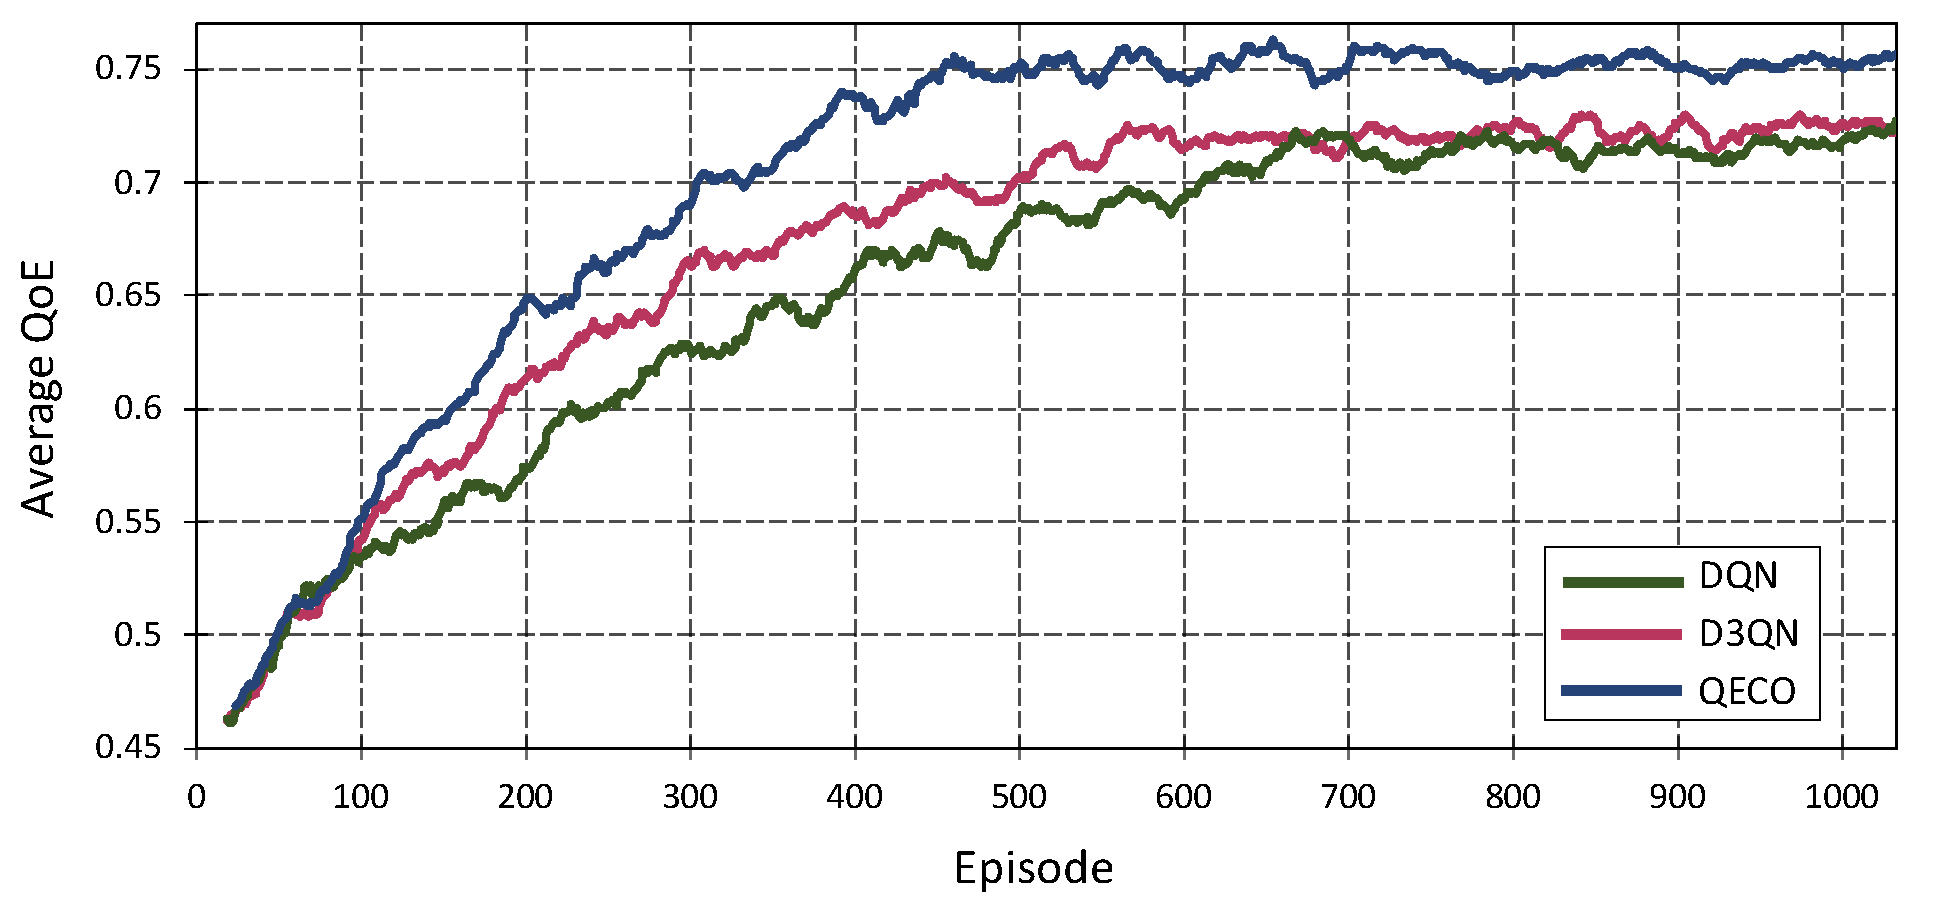
\includegraphics[width=.6\linewidth]{m1}
	\vspace*{-3mm}
	\caption{\textcolor{blue}{The convergence of the average QoE across episodes under different DQN-based methods.}}
	\vspace*{-3mm}
	\label{chart000}
\end{figure}

		\begin{my}{1cm}{1cm}
	\rev{
		{\

	\,\,\,\,We finally delve into the investigation of the convergence performance of the QECO algorithm in Fig.~\ref{chart000} and Fig. 8. To validate the effectiveness of the QECO algorithm, we assess its convergence rate compared to the vanilla DQN and DDQN configurations \cite{van2016deep}, measured by the average QoE across episodes. As shown in Fig.~\ref{chart000}, as the episodes progress, the MD's network learns efficient policies, ultimately stabilizing as it approaches convergence. Specifically, the DQN, DDQN, and our proposed QECO algorithm converge after approximately 650, 550, and 450 iterations, respectively. The QECO algorithm demonstrates the faster convergence while achieves a higher average QoE than the other methods. underscore the beneficial impact of workload prediction by the LSTM network and highlight its effectiveness in efficiently utilizing the processing capabilities of  MDs and ENs.
}}
\end{my}


\vspace{6mm}

\item \underline{Reviewer's Comment}: 
\textit{``(a) In section III, why is the size of the task selected from a discrete set? Is it selected randomly or in another way? Besides, (b) the authors define the offloading indicate function as $y_{i,j}(t)$, it should be involved when modelling the Edge Execution phrase.''} \newline

\underline{Authors' Reply}: (a) Task sizes are chosen from a discrete set as most applications have tasks with predefined sizes. For instance, in image and video processing, tasks are typically divided into standardized sizes~\cite{wang2020intelligent},~\cite{zhang2019toward},~\cite{allahham2022multi}. Therefore, we assume that task sizes are selected randomly and uniformly from this discrete set. To address the reviewer’s comment and to provide further clarity regarding task sizes, we have revised the second paragraph of Section III as follows. \vspace{-3mm}
%The task size is selected randomly from a discrete set to avoid state space complexity. To address the reviewer’s comment, we have added a mention of the random task size selection to the second paragraph of Section II, as follows:
		\begin{my}{1cm}{1cm}
	\rev{
		{\
			
			 \dots

\color{black}
We define $z_i(t)$ as the index assigned to the computation task arriving at MD $i \in \mathcal{I}$ in time slot $t \in \mathcal{T}$. Let $\lambda_i(t)$ denote the size of this task in bits. \textcolor{blue}{The size of task \( z_i(t) \) is selected randomly and uniformly from a discrete set \( \Lambda = \{\lambda_1, \lambda_2, \ldots, \lambda_{\theta}\} \), where \( \theta \) represents the number of these values. Note that task sizes are drawn from a discrete set since, in many applications, tasks typically come with predefined sizes,~\cite{wang2020intelligent},~\cite{zhang2019toward},~\cite{allahham2022multi}. We consider $\lambda_i(t) \in \Lambda \cup \{0\}$ to include the case that no task has arrived.} We also denote the task's processing density as $\rho_i(t)$ that indicates the number of CPU cycles required to complete the execution of a unit of the task. Furthermore, we denote the deadline of this task by $\Delta_i(t)$ which is the number of time slots that the task must be completed to avoid being dropped.

\dots




}}
\end{my} \vspace{3mm}

\setcounter{equation}{13}

(b) Please note that in the original version of the manuscript, we utilized the indicator function $\mathbbm{1}\big(z_{i,j}^{\text{E}}(t') = z_i(t)\big)$ in Equations (21) and (22) to indicate edge server selection. Therefore, there was no need to include offloading indicator $y_{i,j}(t)$. However, to address the reviewer’s comment and make the edge server selection more clear, we have revised Equations (14), (15), (16), and (21) in Section III of the revised manuscript, as follows:\vspace{-7mm}
%Please note that for any queue in the system model, we assume that once a task is completed within a time slot, the next task in the queue will begin processing at the start of the next time slot. Besides, we assume that during each time slot, a mobile device either receives a new task or does not, considering the small duration of each time slot ($\tau = 0.1$ seconds). Based on these assumptions, in the previous version of the manuscript, we utilized the indicator function $\mathbbm{1}\big(z_{i,j}^{\text{E}}(t') = z_i(t)\big)$ in Equations (21) and (22) to indicate edge server selection.
		\begin{my}{1cm}{1cm}
	\rev{
		{\ 
\begin{alignat}{1}
     D_{i,j}^{\text{E}}(t) =  l_{i,j}^{\text{E}}(t)-\hat{l}_{i,j}^{\text{E}}(t).
	\label{14}  
\end{alignat}
\begin{alignat}{1}
    E_{i,j}^{\text{E}}(t) =  \sum_{t^{'}=\hat{l}_{i,j}^{\text{E}}(t)}^{l_{i,j}^{\text{E}}(t)}\hspace{-2mm}{\, p_j^{\text{E}} \tau \over \,\, b_j(t^{'})\,\,}\mathbbm{1}(i \in \mathcal{B}_j(t^{'})), 
	\label{15}  
\end{alignat}
\begin{alignat}{1}
   E_{i}^{\text{I}}(t) =  \sum_{j \in \mathcal{J}}y_{i,j}(t) D_{i,j}^{\text{E}}(t) p_i^{\text{I}} \tau, 
	\label{16}
\end{alignat}
\setcounter{equation}{20}

$\mathcal{E}_i(\boldsymbol{s}_i(t),\boldsymbol{a}_i(t)) = $
	\begin{alignat}{1}
		(1-x_i(t)) E_i^{\text{L}}(t)+ x_i(t) \bigg( E_i^{\text{T}}(t) +   E_i^{\text{I}}(t) +  \sum\limits_{j \in \mathcal{J}}  \sum\limits_{t^{'}=t}^{T}\mathbbm{1}\big(z_{i,j}^{\text{E}}(t') = z_i(t)\big)
		E_{i,j}^{\text{E}}(t')\bigg).
		\label{22}  
\end{alignat}

}}
\end{my} \vspace{3mm}

We have also mentioned the offloading indicated function $y_{i,j}(t)$ explanation in the last paragraph of Section III of the revised manuscript as follows 
		\begin{my}{1cm}{1cm}
	\rev{
		{\ 
\dots 

Recall that $y_{i,j}(t)$ is the offloading indicate function. Moreover, among all $j \in \mathcal{J}$, $y_{i,j}=1$ only for one $j$ which is the corresponding EN.
}}
\end{my}\vspace{5mm}


\item \underline{Reviewer's Comment}: 
\textit{``(a) Some sota methods (e.g., DDQN, DDPG) are expected to be compared in the section on performance evaluation, and authors should have more discussions about the evaluation results rather than merely introducing them.  (b) Besides, I think it is better to design the evaluations with a real dataset. (c) Besides, 9\% and 6\% are not significant improvements compared to other methods.''}\newline


\underline{Authors' Reply}: (a) To address the reviewer's comments, we have extended the evaluation of the QECO algorithm by comparing it with DCDRL \cite{qiu2020distributed}, which is a distributed algorithm for delay-sensitive tasks based on the actor-critic framework. This is the foundation for many state-of-the-art DRL algorithms, including DDPG and PPO. 
We have added this comparison to Section VI of the revised manuscript as follows: 
		\begin{my}{1cm}{1cm}
	\rev{
		{\
			\color{black}
\hspace{-10mm}  \dots \\ We use the following methods as benchmarks.
\begin{itemize}
	
	\item \textbf{Local Computing (LC):} \dots\vspace{1mm}
	
	\item \textbf{Full Offloading (FO):} \dots\vspace{1mm}
	
	\item \textbf{Random Decision (RD):} \dots\vspace{1mm}
	
	\item \textbf{PGOA}~\cite{yang2018distributed}: \dots\vspace{1mm}
	
	\color{blue}
	\item \textcolor{blue}{\textbf{DCDRL}~\cite{qiu2020distributed}: This method is based on the actor-critic framework \cite{NIPS1999_6449f44a}, which underpins many state-of-the-art DRL algorithms, such as DDPG \cite{lillicrap2015continuous}, and PPO \cite{schulman2017proximal}. DCDRL is designed for distributed computation offloading in a queuing-based MEC environment.}
	
	
	
\end{itemize}

}}
\end{my}\vspace{5mm}

	\begin{my}{1cm}{1cm}
	\rev{
		{\small
			\noindent\hspace{-0.5mm}\cite{qiu2020distributed} Qiu, Xiaoyu and Zhang, Weikun and Chen, Wuhui and Zheng, Zibin, ``Distributed and collective deep reinforcement learning for computation offloading: A practical perspective,'' \textit{IEEE Transactions on Parallel and Distributed Systems}, vol. 32, no. 5, pp. 1085--1101, May 2021.\\[10pt]
			\cite{NIPS1999_6449f44a} Konda, Vijay and Tsitsiklis, John, ``Actor-critic algorithms,'' in \textit{Advances in Neural Information Processing Systems}, The {MIT} Press, vol. 12, pp.1008--1014, Apr 1999.\\[10pt]
			\cite{lillicrap2015continuous} Lillicrap, TP, ``Continuous control with deep reinforcement learning,'' \textit{4th International Conference on Learning Representations, {ICLR}}, vol. abs/1509.02971, May 2016.\\[10pt]
			\cite{schulman2017proximal} Schulman, John and Wolski, Filip and Dhariwal, Prafulla and Radford, Alec and Klimov, Oleg, ``Proximal policy optimization algorithms,'' \textit{CoRR}, vol. abs/1707.06347, Jul 2017.}\\}
\end{my}




We have also revised the experiment results as bellow: 

\setcounter{figure}{2}

\begin{figure}[H]\centering
	\captionsetup{name=Fig.}
	\begin{minipage}[b]{0.3\linewidth}
		\centering
		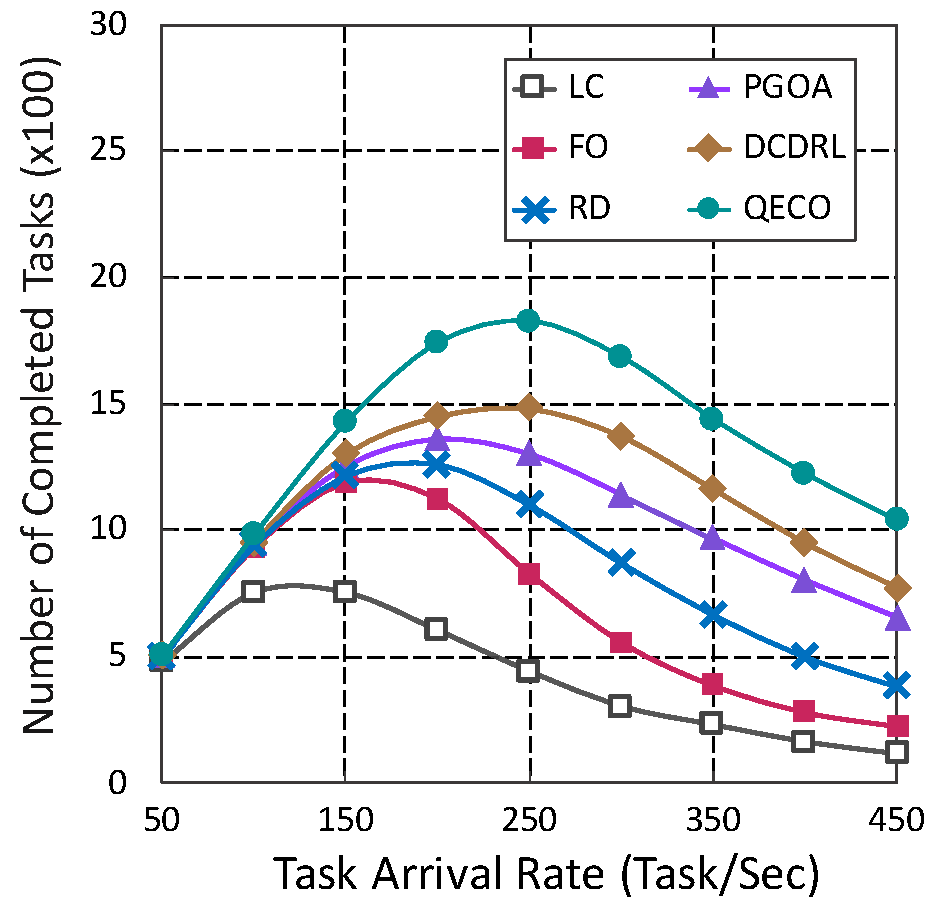
\includegraphics[width=\textwidth]{ drop_1} 
		\textcolor{white}{i}\hspace{0.6cm}(a)
	\end{minipage}
	\hspace{-0.2cm}
	\begin{minipage}[b]{0.3\linewidth}
		\centering
		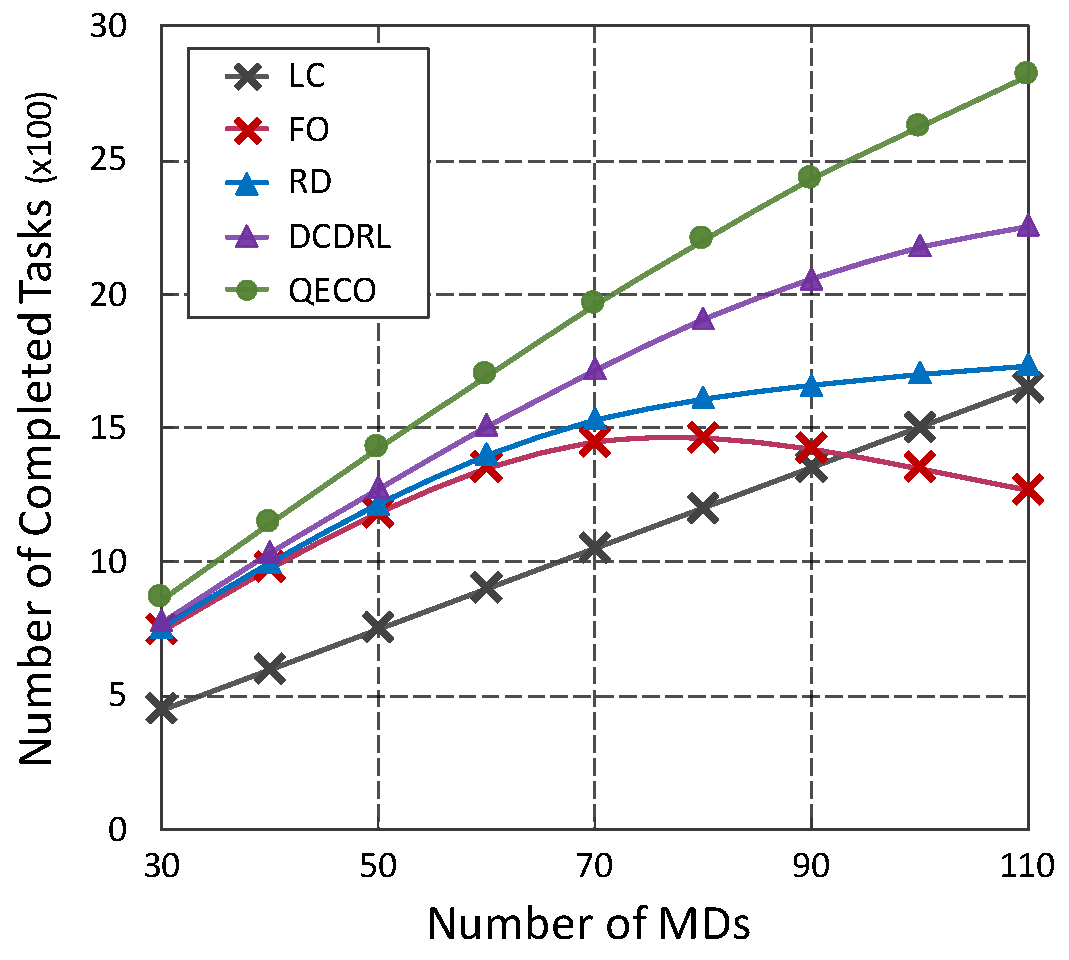
\includegraphics[width=\textwidth]{ drop_2}
		\textcolor{white}{i}\hspace{0.6cm}(b)
	\end{minipage}
	\caption{\textcolor{blue}{The number of completed tasks under different computation workloads: (a) task arrival rate; (b) the number of MDs.}}
	\label{chart1}
\end{figure}\vspace{-8mm}
\begin{figure}[H]\centering
	\captionsetup{name=Fig.}
	\begin{minipage}[b]{0.3\linewidth}
		\centering
		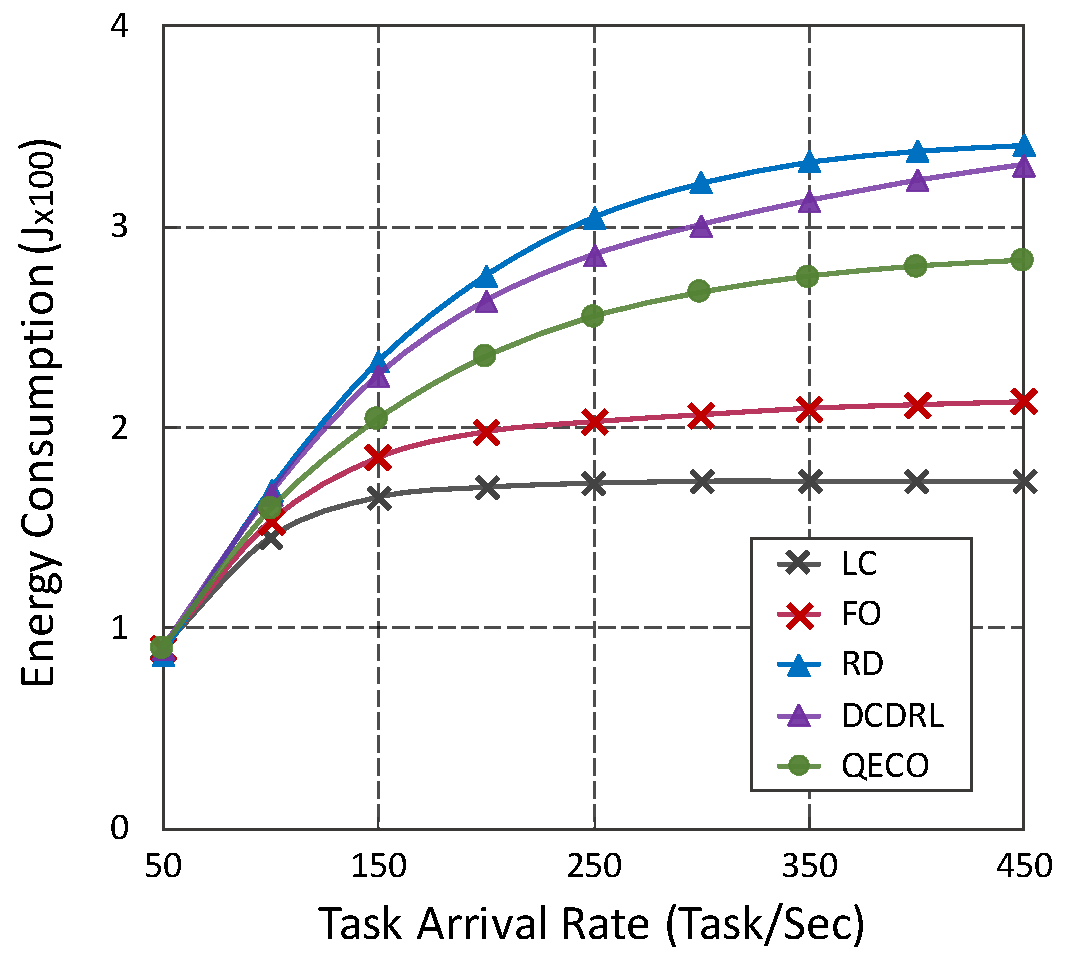
\includegraphics[width=\textwidth]{ energy_1} 		
		\textcolor{white}{i}\hspace{0.6cm}(a)
	\end{minipage}
	\hspace{-0.2cm}
	\begin{minipage}[b]{0.3\linewidth}
		\centering
		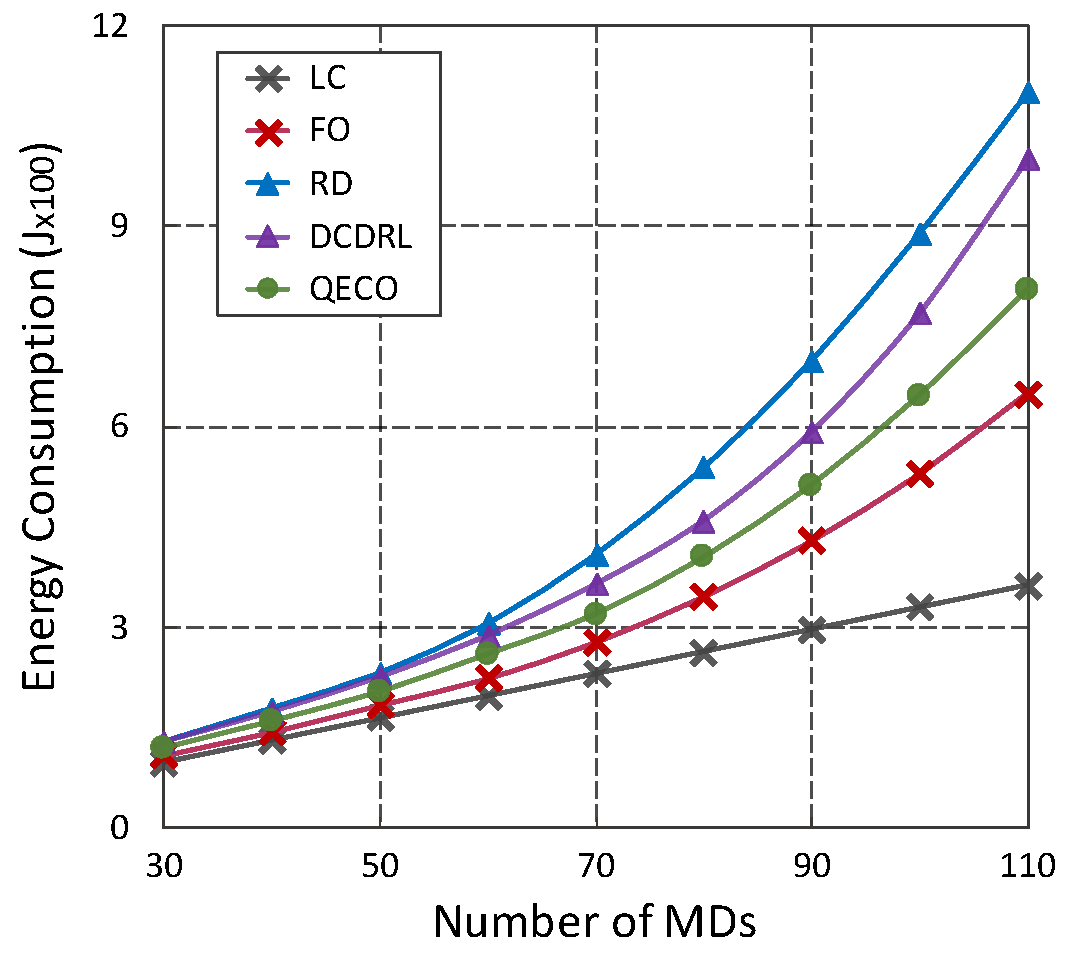
\includegraphics[width=\textwidth]{ energy_2}
		\textcolor{white}{i}\hspace{0.6cm}(b)
	\end{minipage}

	\caption{\textcolor{blue}{The overall energy consumption under different computation workloads: (a) task arrival rate; (b) the number of MDs.}}
	\label{chart2}
\end{figure}\vspace{-8mm}
\begin{figure}[H]\centering
	\captionsetup{name=Fig.}
	\begin{minipage}[b]{0.3\linewidth}
		\centering
		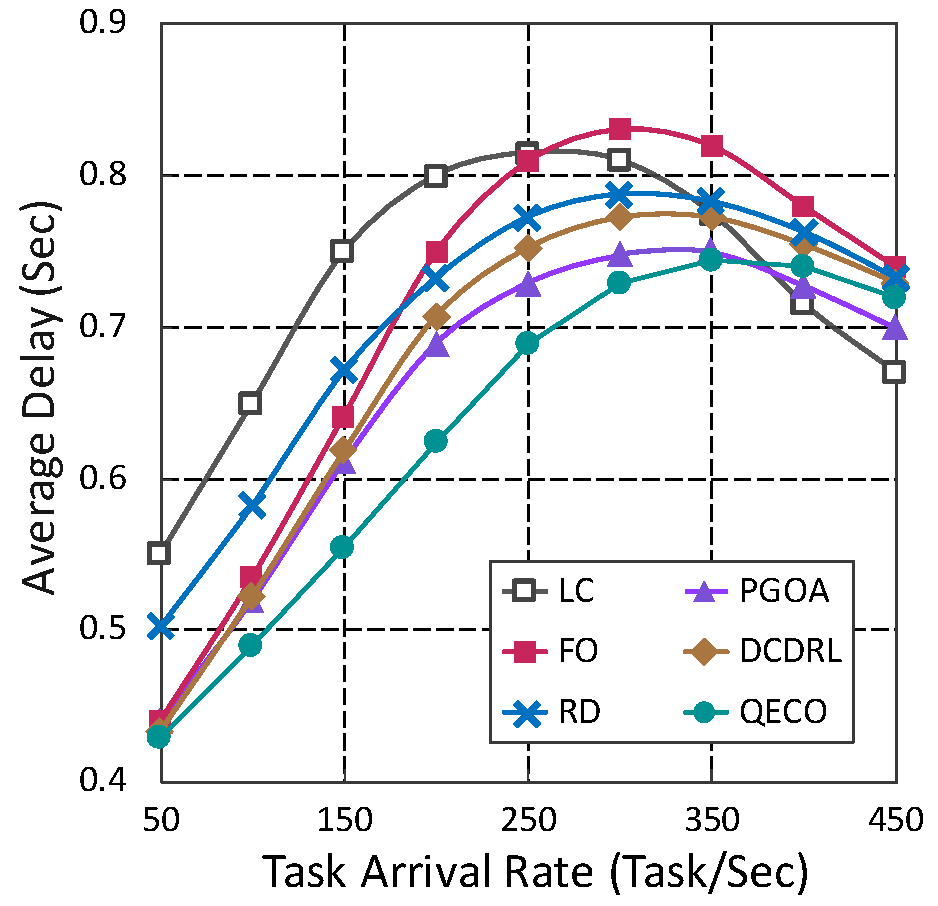
\includegraphics[width=\textwidth]{ delay_1} 		
		\textcolor{white}{i}\hspace{0.6cm}(a)
	\end{minipage}
	\hspace{-0.2cm}
	\begin{minipage}[b]{0.3\linewidth}
		\centering
		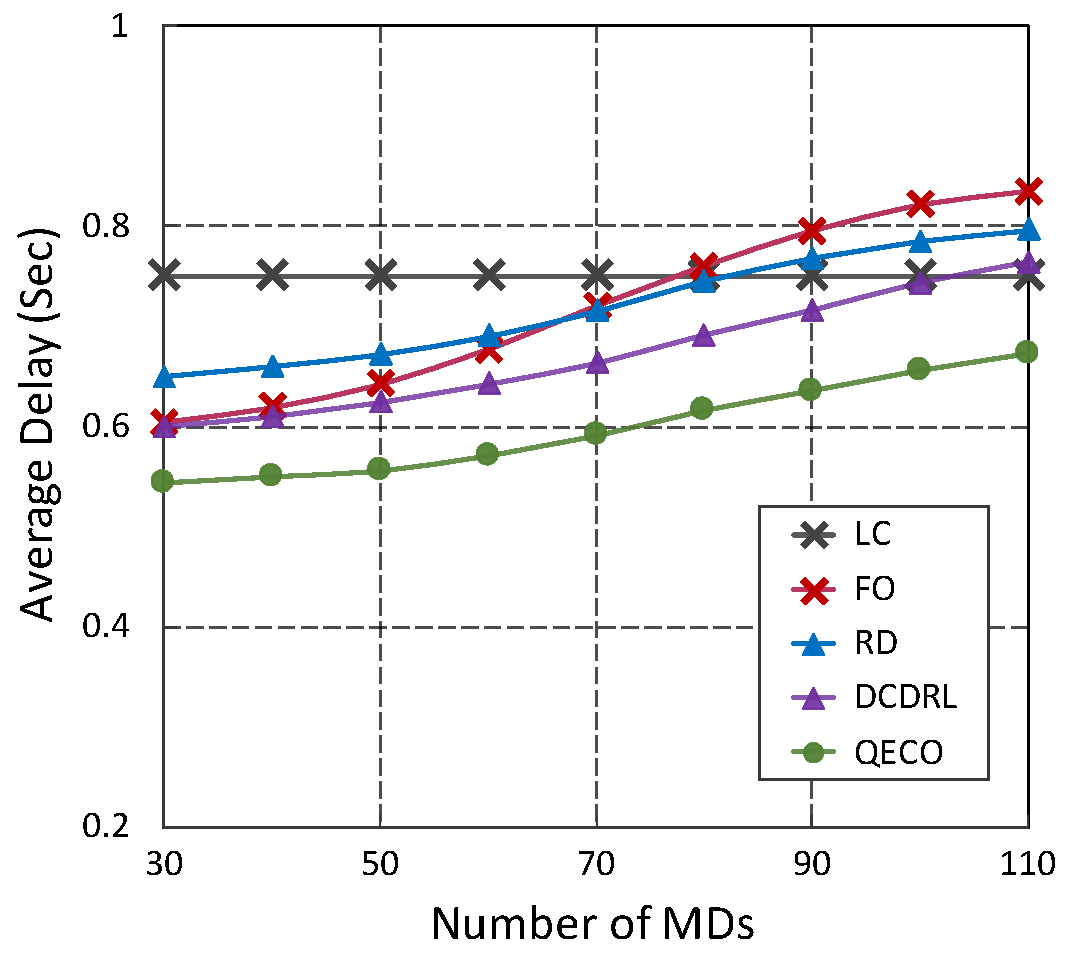
\includegraphics[width=\textwidth]{ delay_2}
		\textcolor{white}{i}\hspace{0.6cm}(b)
	\end{minipage}

	\caption{\textcolor{blue}{The average delay under different computation workloads: (a) task arrival rate; (b) the number of MDs.}}
	\label{chart3}
\end{figure} \vspace{-8mm}
\begin{figure}[H]\centering
	\captionsetup{name=Fig.}
	\begin{minipage}[b]{0.3\linewidth}
		\centering
		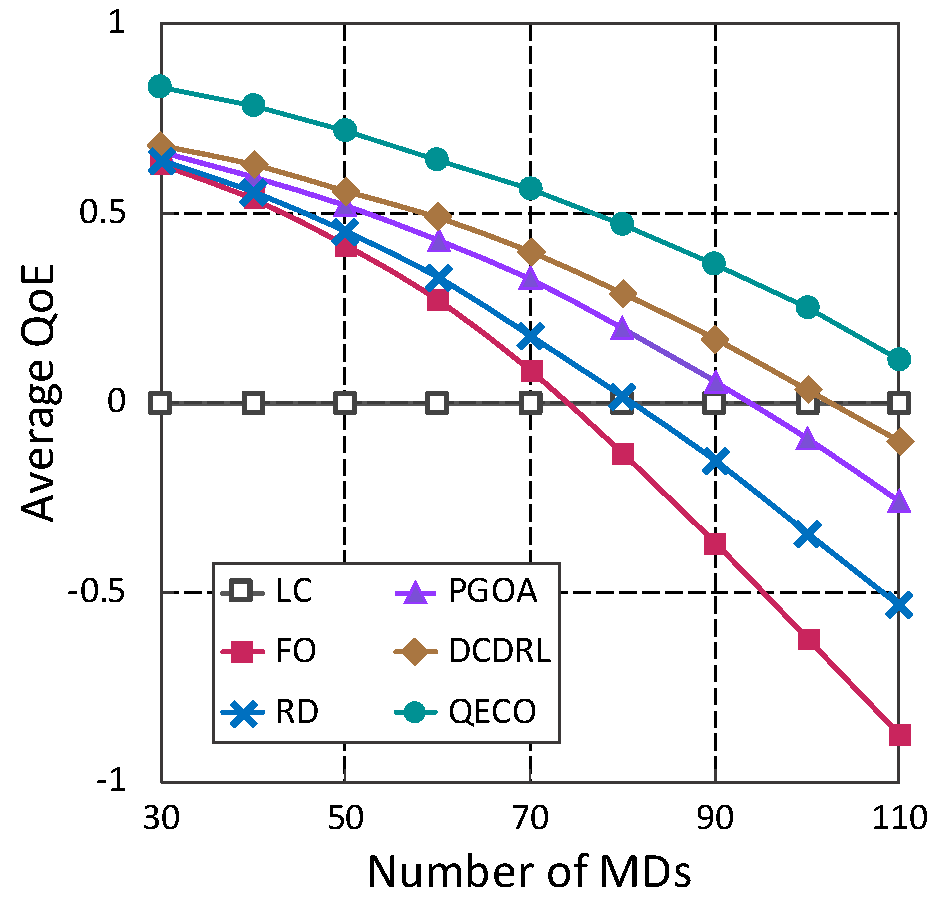
\includegraphics[width=\textwidth]{ qoe_2} 		
		\textcolor{white}{i}\hspace{0.6cm}(a)
	\end{minipage}
	\hspace{-0.2cm}
	\begin{minipage}[b]{0.3\linewidth}
		\centering
		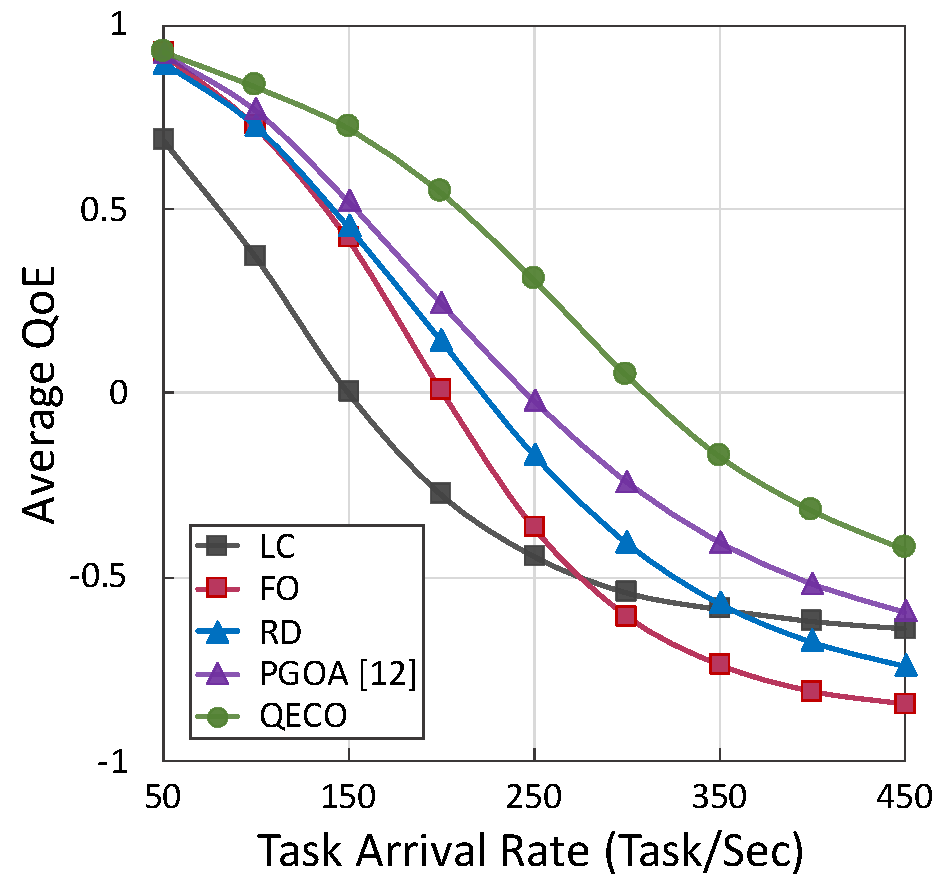
\includegraphics[width=\textwidth]{ qoe_1}
		\textcolor{white}{i}\hspace{0.6cm}(b)
	\end{minipage}

	\caption{\textcolor{blue}{The average QoE under different computation workloads: (a) task arrival rate; (b) the number of MDs.}}
	\label{chart44}
\end{figure} 

Furthermore, to enhance the evaluation of our work, we have extended the performance analysis by comparing QECO with two baseline schemes, vanilla DQN and DDQN \cite{van2016deep}. This comparison illustrates the impacts of the LSTM network and dueling architecture. We have added Fig. 7 to Section VI of the revised manuscript.

\begin{figure}[H]
	\captionsetup{name=Fig.}
	\centering
	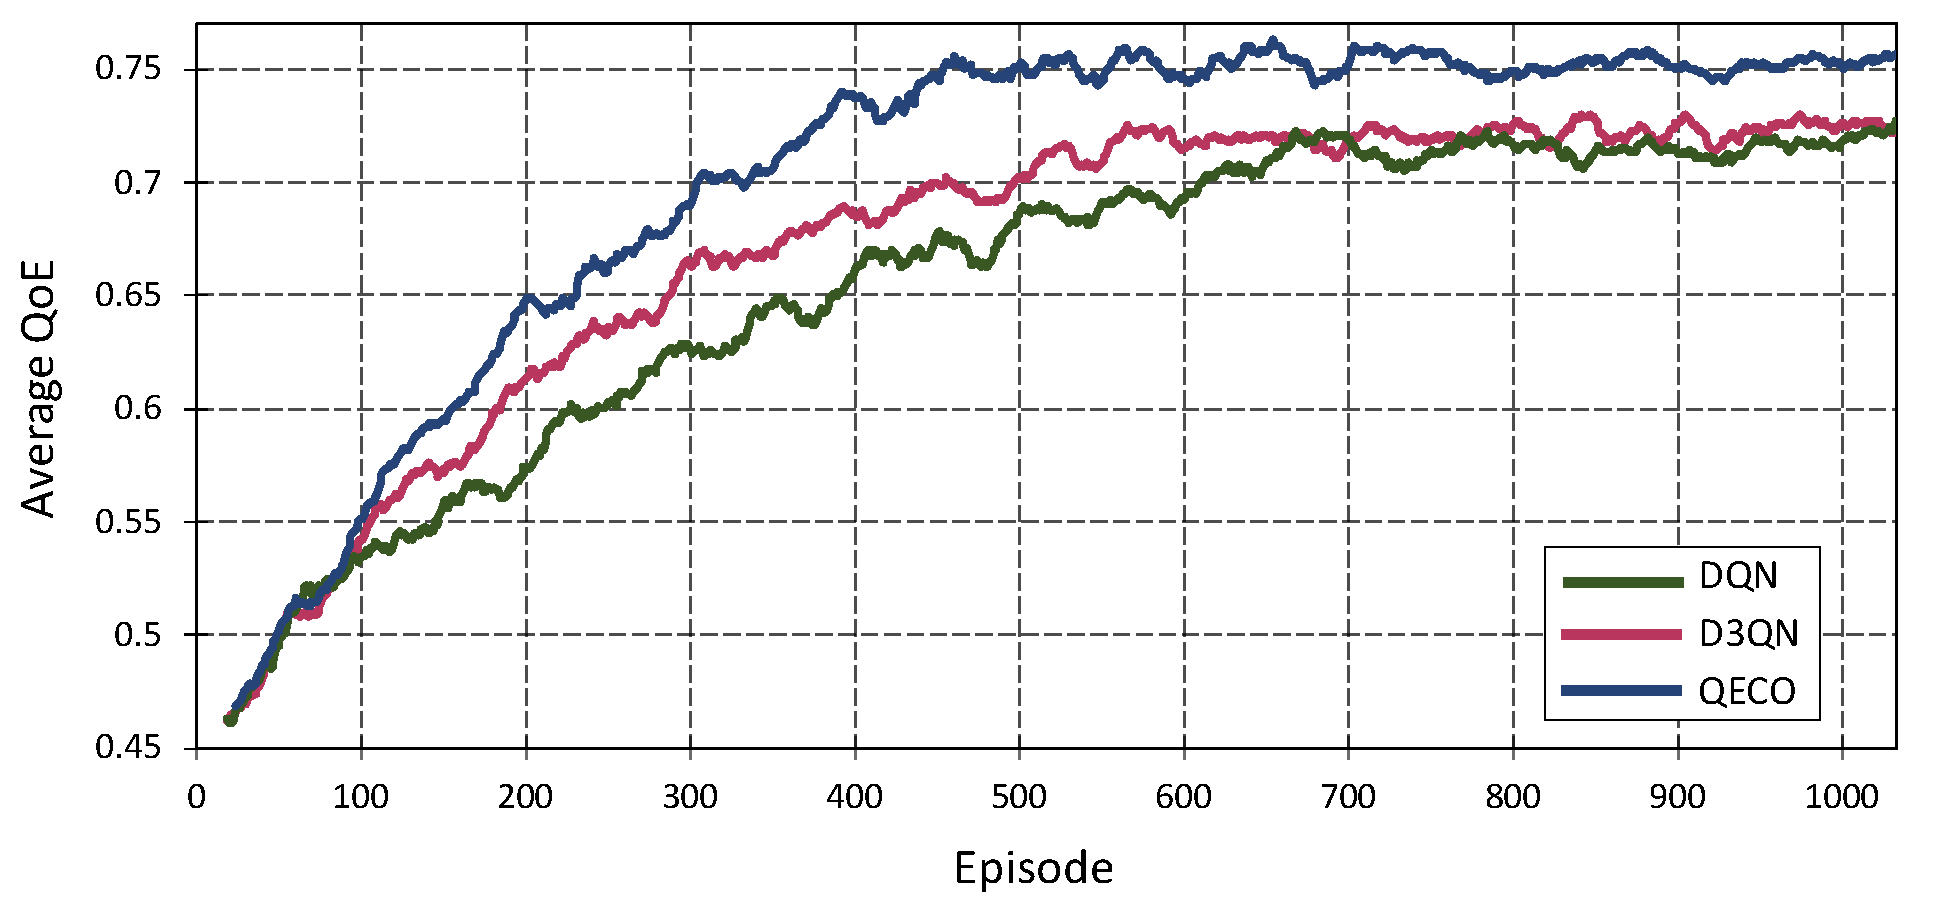
\includegraphics[width=.6\linewidth]{m1}
	\vspace*{-3mm}
	\caption{\textcolor{blue}{The convergence of the average QoE across episodes under different DQN-based methods.}}
	\vspace*{-3mm}
	\label{chart111}
\end{figure}
		\begin{my}{1cm}{1cm}
	\rev{
		{\ 
			
			\dots 


\,\,\,\,We finally delve into the investigation of the convergence performance of the QECO algorithm in Fig.~\ref{chart111} and Fig. 8. To validate the effectiveness of the QECO algorithm, we assess its convergence rate compared to the vanilla DQN and DDQN configurations \cite{van2016deep}, measured by the average QoE across episodes. As shown in Fig.~\ref{chart111}, as the episodes progress, the MD's network learns efficient policies, ultimately stabilizing as it approaches convergence. Specifically, the DQN, DDQN, and our proposed QECO algorithm converge after approximately 650, 550, and 450 iterations, respectively. The QECO algorithm demonstrates the faster convergence while achieves a higher average QoE than the other methods. underscore the beneficial impact of workload prediction by the LSTM network and highlight its effectiveness in efficiently utilizing the processing capabilities of  MDs and ENs. \\\dots }}

\end{my}

\vspace{5mm}

Additionally, to address the reviewer's concern about merely introducing the results, we have revised the performance comparison Subsection in Section VI, as bellow: 


		\begin{my}{1cm}{1cm}
	\rev{ 
		{\ 

\dots \color{black}
			
\,\,\,\,We further investigate the overall improvement achieved by the QECO algorithm in comparison to other methods in terms of the average QoE. This metric signifies the advantages MDs obtain by utilizing different algorithms. \textcolor{blue}{Fig.~\ref{chart44} (a) shows the average QoE for different values of the task arrival rate. This figure highlights the superiority of the QECO algorithm in providing MDs with an enhanced experience. At lower task arrival rates (i.e., 50-150), QECO performs optimally and maintains an average QoE of at least 0.72, while the other methods experience a steeper decline, with average QoE dropping to 0--0.56. Specifically, at a task arrival rate of 200, QECO improves the average QoE by at least 65.7\% compared to other methods in the positive average QoE range. As task arrival rates increase to 300, the average QoE significantly decreases for all methods due to increased competition for resources in the MEC system. However, QECO still maintains a positive average QoE, while other methods fall to negative values, with a decline of up to -0.17. For higher task arrival rates (i.e., 350–450), QECO experiences a negative average QoE, but it shows at least a 42.6\%, 28.5\%, and 22.6\% smaller reduction in average QoE compared to RD, PGOA, and DCDRL, respectively.} \vspace{3mm}



\,\,\,\, Fig.~\ref{chart44} (b) illustrates the average QoE when we increase the number of MDs. The EN's workload grows when there are a larger number of MDs, leading to a reduction in the average QoE of all methods except LC. However, QECO effectively manages the uncertain load at the ENs. \textcolor{blue}{When the number of MDs increases from 30 to 110, QECO consistently maintains at least a 24.8\% higher QoE compared to the other methods. Specifically, at a moderate number of 70 MDs, QECO achieves an average QoE of 0.57, showing a 70.3\% and 44.7\% improvement compared to PGOA and DCDRL, respectively.} It is worth noting that although improvements in each of the QoE factors can contribute to enhancing system performance, it is essential to consider the user's demands in each time slot. Therefore, the key difference between QECO and other methods is that it prioritizes users' demands, enabling it to strike an appropriate balance among them, ultimately leading to a higher QoE for MDs.
 \vspace{3mm}\\\dots }}

\end{my}\vspace{6mm}






(b) We appreciate the reviewer’s suggestion regarding the use of a real dataset for evaluation. Since DRL methods typically rely on data in the form of experience or interaction sequences with an environment, there are no readily available real-world datasets that provide the necessary elements for training DRL algorithms (i.e., state, action, reward, and next state). These interactions involve numerous variables and varying application demands, which are rarely captured in publicly available datasets. Capturing real-world interactions between mobile devices and edge servers would require continuous data collection over an extended period to account for the variability in these factors. Besides, ensuring that the dataset covers all possible scenarios, including rare edge cases, is challenging. To capture the interactions between agents and the environment, we carefully simulated an MEC system that allows the DRL agents to gain experience and generate the data required in the proper format for training. As the agent interacts with the environment, it generates new data at each time step, using the system’s feedback (e.g., QoE) to adjust its actions. \vspace{3mm}

%As mentioned in Section III of the revised manuscript, based on queuing theory, our simulated model provides key system performance metrics (e.g., task delay, energy consumption, etc.), which enable the agent to determine the mobile device's QoE and evaluate each state-action advantage value.\vspace{2mm}





\,\,\,\, For data generation, we adopt a scenario comprising 1,000 episodes. Each episode contains 100 time slots. During each time slot, mobile devices generate computation tasks based on a probabilistic task generation model. The DRL agents make offloading decisions for newly arrived tasks based on their state, which includes information such as task size, queue lengths, the mobile device’s energy level, and the workload history at the edge nodes. The agent evaluates the impact of its actions on the state by assessing the mobile device's QoE, which reflects key performance metrics based on user preferences. The system then transitions to the next state, enabling mobile devices to accumulate the necessary experience through interactions with the MEC environment. As detailed in Section IV-B, these experiences are stored in the replay buffer, creating a rich, continuously growing dataset that represents the diverse conditions and scenarios the agent encounters during computation offloading in MEC. This dynamic, self-generated dataset, by continuous simulation, allows the agent to accumulate a vast and diverse set of training data, representing various interaction sequences between mobile devices and edge servers and ensuring the DRL agent learns optimal strategies for computation offloading.\vspace{2mm}


In response to the reviewer’s comment, we have revised Section VI-A of the revised manuscript to provide further clarity in data generation processes as follows.

\setcounter{subsection}{0}
\setcounter{table}{0}
		\begin{my}{1cm}{1cm}
	\rev{
		{\ 
			
			\dots \color{black} \vspace{-4mm}
			
\subsection{Simulation Setup}
\,\,\,\, We consider a MEC environment with 50 MDs and 5 ENs, similar to \cite{9253665}. We also follow the model presented in \cite{zhou2021deep} to determine the energy consumption. All the parameters are given in Table II. \textcolor{blue}{Since there is no real dataset due to the challenges of capturing representative samples over extended periods, we use a simulated MEC system that enables DRL agents to continuously gather experience and improve their performance based on system feedback (e.g., QoE).} To train the MDs' neural networks, we adopt a scenario comprising 1000 episodes. Each episode contains 100 time slots, each of length 0.1 second. The QECO algorithm incorporates real-time experience into its training process to continuously enhance the offloading strategy. Specifically, we employ a batch size of 16, maintain a fixed learning rate of 0.001, and set the discount factor $\gamma$ to 0.9. The probability of random exploration gradually decreases from an initial value 1, progressively approaching 0.01, all of which is facilitated by an RMSProp optimizer. \textcolor{blue}{The algorithm's source code is available at \cite{QECO}}. 


\color{blue}
\dots 

}}

\end{my}


\vspace{6mm}

(c) Indeed, compared to \cite{yang2018distributed}, QECO improves the number of completed tasks by 14.4\% while at the same time reduces task delay and energy consumption by 9.2\% and 6.3\%, respectively. These together contribute to a significant improvement of 37.1\% in average QoE compared to \cite{yang2018distributed}. To clarify the improvement obtained by QECO, we have revised the abstract as follows. \vspace{4mm}


%To clarify the simulation results, we have revised the Abstract of the manuscript as follows:


		\begin{my}{1cm}{1cm}
	\rev{
 	\dots 
 	
					Simulation results reveal that compared to the state-of-the-art existing works, QECO increases the number of completed tasks by up to 14.4\%, while simultaneously reducing task delay and energy consumption by 9.2\% and 6.3\%, respectively. Together, these improvements align with user preferences, resulting in a significant average QoE enhancement of 37.1\%. This substantial improvement is achieved by accurately accounting for user dynamics and edge server workloads while making intelligent offloading decisions. This highlights QECO's effectiveness in enhancing MEC systems.}

	


\end{my}\vspace{6mm}

We have also revised Section I and Section VI of the revised manuscript to clarify the QECO's improvement, as mentioned in our response to the Reviewer's Comment 2 and 4, respectively.








\vspace{5mm}

\item \underline{Reviewer's Comment}: 
\textit{``Other concerns are also expected to be addressed: (a) be careful to use words like "battery level" to express the energy consumption, because some of the energy is provided by the wired line power. (b) Most of the references are out of 3 years, please investigate more studies published in recent years. (c) The authors should thoroughly check the writing style, grammar, and spelling to enhance the paper's clarity, conciseness, and overall impact.}''\newline

\underline{Authors' Reply}: (a) We have avoided using "battery level" to express the energy consumption and carefully repaced the phrase "battery level" with "energy level of the battery" throughout the revised manuscript. We have also revised the explanation of MD operation modes in Section IV of the revised manuscript as follows. 

		\begin{my}{1cm}{1cm}
	\rev{
		
		\dots
		
Since MDs are assumed to be battery-operated, their operation modes are aligned with those of real-world devices. Let $\phi_i(t)$ represent the \textcolor{blue}{battery level percentage of MD $i$} at time slot $t$, where $\phi_i(t)$ is selected from the discrete set $\Phi = \{\phi_1, \phi_2, \phi_3\}$, corresponding to ultra power-saving, power-saving, and performance modes, respectively.
}
\end{my}\vspace{6mm}

(b) To address the reviewer’s comment, we have removed a few outdated references and cited 17 recently published papers as follows. \newline

		\begin{my}{1cm}{1cm}
	\rev{
		{\small
			\noindent\hspace{-0.1mm}\cite{guo2022energy} M. Guo, Q. Li, Z. Peng, X. Liu, and D. Cui, ``Energy harvesting computation offloading game towards minimizing delay for mobile edge computing,'' \textit{Computer Networks}, vol. 204, pp. 108678, 2022.\\[6pt]
			\cite{tang2022uav} Q. Tang, L. Liu, C. Jin, J. Wang, Z. Liao, and Y. Luo, ``An UAV-assisted mobile edge computing offloading strategy for minimizing energy consumption,'' \textit{Computer Networks}, vol. 207, pp. 108857, 2022.\\[6pt]
			\cite{li2022joint} Y. Li, B. Yang, H. Wu, Q. Han, C. Chen, and X. Guan, ``Joint offloading decision and resource allocation for vehicular fog-edge computing networks: A contract-stackelberg approach,'' \textit{IEEE Internet Things J.}, vol. 9, no. 17, pp. 15969--15982, 2022.\\[6pt]
			\cite{zhang2023multi} J. Zhang, F. Shen, L. Tang, F. Yan, F. Qin, and C. Wang, ``A Multi-Agent Reinforcement Learning Approach for Dynamic Offloading with Partial Information-Sharing in IoT Networks,'' \textit{2023 IEEE 98th Vehicular Technology Conference (VTC2023-Fall)}, pp. 1--5, 2023.\\[6pt]
			\cite{lin2022multi} S.-Y. Lin, C.-M. Huang, and T.-Y. Wu, ``Multi-access edge computing-based vehicle-vehicle-RSU data offloading over the multi-RSU-overlapped environment,'' \textit{IEEE Open J. Intell. Transp. Syst.}, vol. 3, pp. 7--32, 2022.\\[6pt]
			\cite{wei2023many} Z. Wei, B. Li, R. Zhang, X. Cheng, and L. Yang, ``Many-to-many task offloading in vehicular fog computing: A multi-agent deep reinforcement learning approach,'' \textit{IEEE Trans. Mob. Comput.}, vol. 23, no. 3, pp. 2107--2122, 2023.\\[6pt]
			\cite{yuan2023adaptive} S. Yuan, B. Dong, H. Lvy, H. Liu, H. Chen, C. Wu, S. Guo, Y. Ding, and J. Li, ``Adaptive incentivize for cross-silo federated learning in IIoT: A multi-agent reinforcement learning approach,'' \textit{IEEE Internet Things J.}, 2023.\\[6pt]
			\cite{wu2023computation} G. Wu, H. Wang, H. Zhang, Y. Zhao, S. Yu, and S. Shen, ``Computation offloading method using stochastic games for software-defined-network-based multiagent mobile edge computing,'' \textit{IEEE Internet Things J.}, vol. 10, no. 20, pp. 17620–17634, Oct. 2023.\\[6pt]
			\cite{chen2021drl} J. Chen, H. Xing, Z. Xiao, L. Xu, and T. Tao, ``A DRL agent for jointly optimizing computation offloading and resource allocation in MEC,'' \textit{IEEE Internet Things J.}, vol. 8, no. 24, pp. 17508--17524, 2022.\\[6pt]
			\cite{tang2022double} Tang, Huijun and Wu, Huaming and Qu, Guanjin and Li, Ruidong, ``Double deep Q-network based dynamic framing offloading in vehicular edge computing,'' \textit{IEEE Trans. Netw. Sci. Eng.}, vol. 10, no. 3, pp. 1297--1310, May 2022.\\[6pt]
			\cite{wu2024privacy} G. Wu, X. Chen, Z. Gao, H. Zhang, S. Yu, and S. Shen, ``Privacy-preserving offloading scheme in multi-access mobile edge computing based on MADRL,'' \textit{J. Parallel Distrib. Comput.}, vol. 10, no. 1, pp. 451--460, Mar. 2022.\\[6pt]
			\cite{li2020joint} Li, Shilu and Li, Baogang and Zhao, Wei, ``Joint optimization of caching and computation in multi-server NOMA-MEC system via reinforcement learning,'' \textit{IEEE Access}, vol. 8, pp. 112762--112771, Jun 2020.\\[6pt]
			\cite{munir2021multi} M. S. Munir, N. H. Tran, W. Saad, and C. S. Hong, ``Multi-agent meta-reinforcement learning for self-powered and sustainable edge computing systems,'' \textit{IEEE Trans. Netw. Serv. Manag.}, vol. 18, no. 3, pp. 3353-3374. 2021.\\[6pt]
			\cite{wu2024combining} G. Wu, X. Chen, Y. Shen, Z. Xu, H. Zhang, S. Shen, and S. Yu,``Combining Lyapunov optimization with Actor-Critic networks for privacy-aware IIoT computation offloading,'' in \textit{IEEE Internet Things J.}, 2024, Early Access\\[6pt]
			\cite{li2022integrated} Li, Xian and Huang, Liang and Wang, Hui and Bi, Suzhi and Zhang, Ying-Jun Angela, ``An integrated optimization-learning framework for online combinatorial computation offloading in MEC networks,'' \textit{IEEE Wirel. Commun.}, vol. 29, no. 1, pp. 170--177, Feb 2022.\\[6pt]
			\cite{wang2020reinforcement} Wang, Dongyu and Tian, Xinqiao and Cui, Haoran and Liu, Zhaolin, ``Reinforcement learning-based joint task offloading and migration schemes optimization in mobility-aware MEC network,'' \textit{China Commun.}, vol. 17, no. 8, pp. 31--44, Aug 2020.\\[6pt]
			\cite{wu2023multi} G. Wu, Z. Xu, H. Zhang, S. Shen, and S. Yu,  ``Multi-agent DRL for joint completion delay and energy consumption with queuing theory in MEC-based IIoT,'' in \textit{J. Parallel Distrib. Comput.}, vol. 176, pp. 80–94, Jun. 2023.
			\\[6pt]}}
\end{my}



	We have also cited these works in the following sentences in Sections I and II of the revised manuscript.\newline
	
\begin{my}{1cm}{1cm}
		\rev{
			{
	
	\dots
	
	\textcolor{blue}{	\,\,\,\, In addition, QoE is a time-varying performance measure that reflects user satisfaction and is not affected only by delay \cite{guo2022energy}, but also by energy consumption \cite{tang2022uav}. Albeit some existing works have investigated the trade-off between delay and energy consumption \cite{li2022joint}, they fail to properly estimate the QoE value and address the user demands and requirements. }
	
	\dots
	
	  In recent years, numerous studies have focused on computation offloading in MEC, covering a broad range of applications, including IoTs \cite{zhang2023multi}, Internet of Vehicles (IoVs) \cite{lin2022multi}, \cite{wei2023many}, and Industrial IoT (IIoT) \cite{yuan2023adaptive}. 

	\dots


	Recent research has extensively explored single-objective optimization in the context of MEC, focusing on optimizing a single objective, such as delay or energy consumption. 
    Given the dynamic nature of MEC systems, in \cite{li2022integrated} the authors proposed an integrated optimization framework, which leverages past experience and model knowledge to enable fast and resilient real-time offloading control. Li \textit{et al.} in \cite{li2020joint} introduced a DRL-based delay-optimal offloading strategy that employs a DQN to learn offloading decisions autonomously. 
	To minimize total delay and reduce mobile vehicle task waiting time, Tang \textit{et al.} in \cite{tang2022double} developed a dynamic offloading model for multiple mobile vehicles, segmenting tasks into sequential subtasks for more precise offloading decisions.
	\dots
	To minimize energy consumption, Munir \textit{et al.} \cite{munir2021multi} developed a semi-distributed approach using a multi-agent RL framework for self-powered MEC. 
	\dots
	Wang et al. in \cite{wang2020reinforcement} studied the computation offloading problem in MEC systems within cellular networks, emphasizing mobile awareness. They proposed a joint approach for task offloading and computation allocation, aiming to address the task offloading costs associated with user mobility. 

	\dots


	In MEC environments, multiple objectives often compete, requiring a balance in decision-making. 
	\dots 
	Chen \textit{et al.} in \cite{chen2021drl} addressed a joint optimization problem involving computation offloading and resource allocation, aiming to reduce both task processing delay and energy consumption across all MDs.
	To optimize privacy protection and quality of service, authors in \cite{wu2024privacy} investigated the joint computation offloading and power allocation problems for the IIoT network. They modeled the problem as an MDP and proposed a multi-agent DQN-based algorithm. 
    \dots
	Wu \textit{et al.} in \cite{wu2023computation} introduced a stochastic game-based resource allocation in the SDN-based MEC network. They used an MDP and proposed a multi-agent RL method to minimize both energy consumption and processing delay. 

	\dots
	
	To further enhance the modeling of real-world scenarios, some studies have applied queuing theory to model MEC systems, which helps capture the dynamic nature of the network and allows MEC systems to allocate computational and transmission resources more efficiently.
    \dots
	To address the privacy-aware computation offloading problem, Wu \textit{et al.} in \cite{wu2024combining} modeled the problem as an MDP and proposed a DQN-based method to optimize the computation rate and energy consumption in a queuing-based IIoT network.\dots
    Wu \textit{et al.} in \cite{wu2023multi} investigated the computation offloading problem in a queuing-based MEC IIoT system. They modeled the problem as a POMDP and proposed a multi-agent proximal policy optimization (PPO)-based method to obtain the optimal offloading strategy in dynamic environments.
	In \cite{gao2022large}, Gao \textit{et al.} introduced an attention-based multi-agent algorithm designed for decentralized computation offloading.
	
	
	
}}
\end{my}\vspace{6mm}

We have provided a survey of the recently published state-of-the-art works in Section II of the revised manuscript, as mentioned in our response to Reviewer's Comment 1.\newline

(c) We have thoroughly reviewed the writing style, grammar, and spelling, and have carefully proofread the manuscript. We trust that all issues have been addressed in this revised version. 

\vspace{10mm}



\end{enumerate}

\textit{We would like to gratefully thank the reviewer for the valuable comments and suggestions. We hope that we have satisfactorily addressed these comments.}\newline




	\setcounter{section}{1}
\setcounter{table}{0}

\section{Response to Reviewer 2}
\begin{enumerate}
	
	\item \underline{Reviewer's Comment}: 
	\textit{``(a) The authors should provide a comparative table to highlight their contributions. (b) Specially, the authors should compare their method with other references on computation task offloading cited in the paper, including aspects such as scenarios, methods, advances, drawbacks, and so on.''} \newline

	\underline{Authors' Reply}: (a) To address the reviewer's comment, we have carefully studied the recently published papers and revised the manuscript accordingly. 
	To be more specific, we have extended the literature review in Section II of the revised manuscript by providing a more comprehensive survey of the recently published state-of-the-art works and comparing their characteristics in Table \ref{table11}.
	We have also compared our work with more existing works and extended the performance evaluation in Section VI of the revised manuscript. 


\vspace{3mm}
 The newly added Section II of the revised manuscript is as follows. As suggested by the reviewer, we have also included Table I that summarizes the existing works.
	
\begin{my}{1cm}{1cm}
	\rev{\setcounter{section}{1}
		\section{Related Work}
		\label{section:II}
		
		\,\,\,\,
		In recent years, numerous studies have focused on computation offloading in MEC, covering a broad range of applications, including IoTs \cite{zhang2023multi}, Internet of Vehicles (IoVs) \cite{lin2022multi}, \cite{wei2023many}, and Industrial IoT (IIoT) \cite{yuan2023adaptive}. 
		To effectively tackle the challenges of MEC arising from the ever-changing nature of networks, recent research highlights the effectiveness of DRL in adapting to environmental changes and learning optimal strategies. In this section, we explore the current DRL-based state-of-the-art works and discuss their strengths and limitations. Table~\ref{table1} provides an intuitive comparison of these works.
		\subsection{DRL-based Optimization Methods for MEC} 
		
		\,\,\,\,
		There are two primary categories of related research in resource management for MEC based on target objectives, single-objective optimization and multi-objective optimization methods, where RL are mainstream optimization techniques.\vspace{3mm}
		\subsubsection{Single-Objective Optimization} 
		Recent research has extensively explored single-objective optimization in the context of MEC, focusing on optimizing a single objective, such as delay or energy consumption. 
		Given the dynamic nature of MEC systems, in \cite{li2022integrated} the authors proposed an integrated optimization framework, which leverages past experience and model knowledge to enable fast and resilient real-time offloading control. 
		Li \textit{et al.} in \cite{li2020joint} introduced a DRL-based delay-optimal offloading strategy that employs a DQN to learn offloading decisions autonomously. 
		To minimize total delay and reduce mobile vehicle task waiting time, Tang \textit{et al.} in \cite{tang2022double} developed a dynamic offloading model for multiple mobile vehicles, segmenting tasks into sequential subtasks for more precise offloading decisions.
		Sun \textit{et al.} in \cite{sun2024hierarchical} explored both computation offloading and service caching problems in MEC. They formulated an optimization problem that aims to minimize the long-term average service delay. They then proposed a hierarchical DRL framework, which effectively handles both problems under heterogeneous resources.
		To minimize energy consumption, Munir \textit{et al.} \cite{munir2021multi} developed a semi-distributed approach using a multi-agent RL framework for self-powered MEC. 
		Zhou \textit{et al.} in \cite{zhou2021deep} proposed a Q-learning approach, which is an extension of RL to achieve optimal resource allocation strategies and computation offloading.
		Wang et al. in \cite{wang2020reinforcement} studied the computation offloading problem in MEC systems within cellular networks, emphasizing mobile awareness. They proposed a joint approach for task offloading and computation allocation, aiming to address the task offloading costs associated with user mobility. 
		In \cite{zhao2019deep}, Zhao \textit{et al.} proposed a computation offloading algorithm based on DRL, which addresses the competition for wireless channels to optimize long-term downlink utility.
		Dai \textit{et al.} in \cite{dai2020edge} introduced the integration of action refinement into DRL and designed an algorithm based on deep deterministic policy gradient (DDPG) to optimize resource allocation and computation offloading concurrently.\vspace{3mm}
		
		
		
		
		\subsubsection{Multi-Objective Optimization.}
		In MEC environments, multiple objectives often compete, requiring a balance in decision-making. For instance, task offloading must carefully navigate trade-offs between delay and energy consumption, as well as balance energy usage against the number of completed tasks. Research has increasingly addressed these multi-objective optimization challenges.
		Chen \textit{et al.} in \cite{chen2021drl} addressed a joint optimization problem involving computation offloading and resource allocation, aiming to reduce both task processing delay and energy consumption across all MDs.
		To optimize privacy protection and quality of service, authors in \cite{wu2024privacy} investigated the joint computation offloading and power allocation problems for the IIoT network. They modeled the problem as an MDP and proposed a multi-agent DQN-based algorithm. 
		Huang \textit{et al.} in \cite{huang2019deep}, focused on a wireless-powered MEC and proposed a DRL-based approach, capable of attaining near-optimal decisions. This is achieved by selectively considering a compact subset of candidate actions in each iteration. 
		Liu \textit{et al.} in \cite{liu2021learn} investigated a two-timescale computing offloading and resource allocation problem and proposed a resource coordination algorithm based on multi-agent DRL, which can generate interactive information along with resource decisions. 
		Wu \textit{et al.} in \cite{wu2023computation} introduced a stochastic game-based resource allocation in the SDN-based MEC network. They used an MDP and proposed a multi-agent RL method to minimize both energy consumption and processing delay. 
		In \cite{Bolourian-WCL24}, the authors proposed an offloading algorithm using deep Q-learning for wireless-powered IoT devices in MEC systems. This algorithm aims to minimize the task drop rate while the devices solely rely on harvested energy for operation. \vspace{3mm}
		
		\,\,\,\,
		To further enhance the modeling of real-world scenarios, some studies have applied queuing theory to model MEC systems, which helps capture the dynamic nature of the network and allows MEC systems to allocate computational and transmission resources more efficiently.
		Liao \textit{et al.} in \cite{liao2023online} introduced a double DQN (DDQN)-based algorithm for performing online computation offloading in MEC. This algorithm optimizes transmission power and scheduling of CPU frequency when minimizing both task computation delay and energy consumption. 
		To address the privacy-aware computation offloading problem, Wu \textit{et al.} in \cite{wu2024combining} modeled the problem as an MDP and proposed a DQN-based method to optimize the computation rate and energy consumption in a queuing-based IIoT network.
		Huang \textit{et al.} in \cite{huang2021deadline} proposed a DRL-based method based on a partially observable MDP (POMDP), which guarantees the deadlines of real-time tasks while minimizing the total energy consumption of MDs. This algorithm effectively tackles the challenges of dynamic resource allocation in large-scale heterogeneous networks. 
		Tang \textit{et al.} in \cite{9253665} investigated the task offloading problem for indivisible and deadline-constrained computational tasks in MEC systems. The authors proposed a distributed DRL-based offloading algorithm designed to handle uncertain workload dynamics at the ENs. 
		Gong \textit{et al.} in \cite{gong2022edge} proposed a DRL-based network structure in the IIoT systems to jointly optimize task offloading and resource allocation to achieve lower energy consumption and decreased task delay.
		To optimize delay and energy consumption, Wu \textit{et al.} in \cite{wu2023multi} investigated the computation offloading problem in a queuing-based MEC IIoT system. They modeled the problem as a POMDP and proposed a multi-agent proximal policy optimization (PPO)-based method to obtain the optimal offloading strategy in dynamic environments.
		In \cite{gao2022large}, Gao \textit{et al.} introduced an attention-based multi-agent algorithm designed for decentralized computation offloading.
		\begin{table*}[tbp]\textcolor{blue}{
				\renewcommand{\arraystretch}{0.2}
				\captionsetup{name=TABLE}
				\caption{\textcolor{blue}{Comparison of Related Works \vspace{4mm}}}
				\scalebox{0.7}{%
					\begin{tabular}{ lp{7cm}p{6cm}p{4cm}p{6cm}l} 
						\toprule
						\textbf{Paper}  &  \textbf{Problem} &  \textbf{Objective} & \textbf{Method} &  \textbf{Limitation}  \\ \midrule
						\cite{li2022integrated} & Online computation offloading & Minimize computation delay & Actor-critic network & Not consider system energy consumtion \\ \midrule
						\cite{li2020joint} & Caching and computation offloading & Minimize delay of the whole system &  Multi-agent DQN & Not consider system energy consumtion \\ \midrule
						\cite{tang2022double}  & Computation offloading & Minimize total delay & DDQN & Not consider system energy consumtion \\ \midrule
						\cite{wang2020reinforcement} & Mobility aware computation offloading & Minimize energy consumtion & Q-learning & Not consider computation delay\\ \midrule
						\cite{liu2021learn}  & Resource allocation and computation offloading & Minimize execution cost  & Multi-agent actor-critic network &  Not consider delay-sensitive tasks \\\midrule
						\cite{wu2023computation}   & Stochastic game-based resource allocation & Minimize energy consumption and processing delay & Multi-agent RL & Not consider tasks with maximum delay tolerance\\\midrule
						\cite{zhou2021deep} & Resource allocation and computation offloading & Minimize energy consumption of the entire system & DDQN & Only for a single MEC system model \\\midrule				
						%\cite{huang2019deep} & Wireless-powered MEC & Computation offloading and resource allocations & Maximize computation rate & MIP & DQN & Not consider delay-sensitive tasks \\\midrule
						\cite{wu2024privacy} & Joint power allocation and computation offloading  & Optimization of privacy protection and quality of service.  & Multi-agent actor-critic network& Not take user's demand into consideration \\\midrule
						\cite{dai2020edge} & Resource allocation and computation offloading & Minimize energy consumption & DDPG & Not take user's demand into consideration \\\midrule
						\cite{zhao2019deep} & User association and resource allocation & Optimize downlink utility  & Multi-agent D3QN & Not consider system delay and energy consumtion \\\midrule
						\cite{liao2023online}  & Online computation offloading & Minimize computation delay and energy consumption & DDQN & Only for a single MEC system model  \\\midrule
						\cite{wu2024combining}   & Privacy aware computation offloading & Optimization of computation rate and energy consumption  & Actor-critic network  & Not take user's demand into consideration \\\midrule
						\cite{Bolourian-WCL24}  & Energy harvesting  computation offloading & Minimize drop rate and energy consumption.  & DQN & Not consider computation delay  \\\midrule
						\cite{huang2021deadline}  & Computation offloading & Optimize drop rate and energy consumption & DDPG & Not consider computation delay \\ \midrule
						\cite{gong2022edge} & Resource allocation and computation offloading & Minimize task computation delay and energy consumption  & DRL & Not take user's demand into consideration\\\midrule
						\cite{sun2024hierarchical} & Computation offloading and service caching & Minimize average service delay & Hierarchical DRL & Not consider system energy consumtion \\\midrule
						\cite{wu2023multi}  & Computation offloading & Optimize delay and energy consumption  & Multi-agent PPO&  Not consider tasks with maximum delay tolerance \\\midrule
						\cite{9253665}  &  Computation offloading & Minimize drop rate and computation delay.  & D3QN + LSTM & Not consider system energy consumtion\\\midrule
						\cite{gao2022large}  & Decentralized computation offloading & Optimize system cost and completion rates  & Multi-agent actor-critic network& Not take user's demand into consideration \\\midrule
						QECO  &  Computation offloading & Maximize the QoE of each MD individually & D3QN + LSTM & \\
						\toprule
				\end{tabular}}
				\label{table1}}
		\end{table*}
		\subsection{Analysis and Motivation}
		\,\,\,\,
		Despite extensive research efforts, task offloading continues to encounter significant challenges in real-world scenarios involving multiple MDs and ENs. We discuss these challenges from two aspects, i.e., system modeling and target objective optimization. \vspace{3mm}
		
		\subsubsection{System modeling}
		Some existing works primarily focus on simplified MEC networks, investigating single MEC network models. For instance, studies \cite{zhou2021deep}, \cite{liu2021learn} only examine single-server or single-user scenarios, while \cite{huang2019deep}--\cite{wu2023computation} do not account for delay-sensitive tasks. In contrast, our research addresses a more realistic MEC scenario, considering delay-sensitive tasks with processing deadlines. This is challenging due to the interplay between processing deadlines, load dynamics at the ENs, and the resulting offloaded task delays. Additionally, the absence of robust underlying resource scheduling systems can lead to data congestion during transmission and inefficient resource allocation, hindering overall system performance \cite{wang2020reinforcement}--\cite{chen2021drl}. Hence, more accurate MEC models are necessary to handle the complexities of dynamic resource scheduling in large-scale scenarios.
		To better represent real-world scenarios, authors in \cite{Bolourian-WCL24}--\cite{9253665} have applied queuing theory to model MEC systems. This approach helps capture the dynamic nature of networks, enabling MEC systems to allocate computational and transmission resources more efficiently. In a similar vein, we approached the offloading process as a holistic queuing system, where multiple queues ensure fair resource scheduling for MEC, leading to more accurate and efficient resource management.\vspace{3mm}
		
		\,\,\,\,
		In addition, the limited processing capacities of ENs necessitate careful consideration when allocating resources to MDs. The processing capacity allocated to an MD depends on the dynamic workload of an EN at any given time. Some studies have failed to account for these challenges in dynamic network environments, resulting in reduced system performance. For example, in \cite{chen2021drl}, it is assumed that MDs have sufficient transmission and computation resources from ENs, which may not reflect real-world conditions. While the works \cite{zhao2019deep}, \cite{dai2020edge}, and \cite{wu2024privacy} investigated limited resources in MEC, they did not consider dynamic workloads at ENs in decision-making processes, leading to potential performance issues.
		Certain studies such as \cite{sun2024hierarchical}, \cite{gong2022edge}-\cite{gao2022large} have addressed load levels at ENs and proposed task offloading algorithms. However, these algorithms often require global system information, resulting in high signaling overhead. In contrast to these works, we propose a distributed algorithm that effectively manages unknown load dynamics at ENs. This algorithm enables each MD to make offloading decisions independently, without requiring information (e.g., task models, offloading decisions) from other MDs, thereby reducing signaling overhead and improving overall system performance.\vspace{3mm}
		\subsubsection{Optimization Objectives}
		Considering delay and energy consumption as optimization objectives represents a significant research focus in MEC. Most existing studies tend to optimize these two objectives independently, often neglecting the conflicts that arise between them, which can lead to skewed optimization results. Additionally, some research has prioritized maximizing the number of completed tasks, highlighting the advantages that MEC systems offer. Therefore, delay, energy consumption, and the number of completed tasks are critical factors in the design of MEC systems. However, to the best of our knowledge, there has been limited research that simultaneously addresses all three objectives.
		Different from works \cite{li2022integrated}-\cite{dai2020edge}, which only focus on delay-optimal optimization or energy-efficient optimization, we are motivated to emphasize the MEC system with delay, energy consumption, and the number of completed tasks as three objectives for QoE optimization. Multi-objective studies \cite{chen2021drl}-\cite{gao2022large} have mostly investigated the trade-off between two or three of these factors but fail to properly address user demands and fulfill QoE requirements. QoE is a time-varying performance measure that reflects user satisfaction, where each user may have unique QoE requirements according to the Mobile Devices' (MDs) individual preferences.
		In contrast to \cite{li2022integrated}-\cite{gao2022large}, to effectively address personalized QoE optimization, we define an adaptive trade-off between task completion and cost reduction. We introduce a weighted sum between completion delay and energy consumption as an associated cost. Each MD dynamically adjusts these weights to reflect the importance of different factors based on its energy modes. \vspace{3mm}
		
		
		
	}
\end{my}



















\vspace{6mm}

We have also revised Section I accordingly to highlight the contributions and make it consistent with the updated contents of related work. The following paragraphs show the changes we have made in Section I of the revised manuscript.

\begin{my}{1cm}{1cm}
	\rev{
		
		
		\color{black}
		

		\dots 
		
		
		\,\,\,\,
		Efficient task offloading in MEC is a complex optimization challenge due to the dynamic nature of the network and the variety of MDs and servers involved \cite{jiang2019toward} \cite{TNSE-WU-24}. In particular, determining the optimal offloading strategy, scheduling the tasks, and selecting the most suitable EN for task offloading are the main challenges that demand careful consideration. \textcolor{blue}{In addition to the dynamic network changes, the uncertain requirements and sensitive latency properties of computation tasks pose nontrivial challenges that can significantly impact the MEC systems.}\vspace{3mm}
		
		
		\,\,\,\,
		To cope with the dynamic nature of the network, recent research has proposed several task offloading algorithms using machine learning methods. In particular, reinforcement learning (RL) \cite{mnih2015human} holds promises to determine optimal decision-making policies by capturing the dynamics of environments and learning strategies for accomplishing long-term objectives. \textcolor{blue}{However, the traditional RL methods are not efficient to  handle  environments with high-dimensional state  spaces. Deep reinforcement learning (DRL) combines  traditional RL  with  deep  neural  networks  to  intelligently respond to the unknown and dynamic system when addressing the limitations of RL-based algorithms. Despite these advancements, task offloading still faces significant challenges in real-world scenarios with multiple MDs and ENs. In such scenarios, it is essential for MDs to make offloading decisions independently  without prior knowledge of other MDs’ tasks and offloading models. However,  existing works fail to adequately address this challenge. In addition, QoE is a time-varying performance measure that reflects user satisfaction and is not affected only by delay \cite{guo2022energy}, but also by energy consumption \cite{tang2022uav}. Albeit some existing works have investigated the trade-off between delay and energy consumption \cite{li2022joint}, they fail to properly estimate the QoE value and address the user demands and requirements. Although deep Q-networks (DQN) offer a valuable tool, a more comprehensive approach is required to accurately estimate the QoE while addressing the aforementioned challenges in practical scenarios where global information is limited.}\vspace{3mm}
		
		\,\,\,\,
		In this study, we delve into the computation task offloading problem in MEC systems, where strict task processing deadlines and energy constraints can adversely affect the system performance.   \textcolor{blue}{We propose a distributed QoE-oriented computation offloading (QECO) algorithm to efficiently handle task offloading in uncertain loads at ENs.} This algorithm empowers MDs to make offloading decisions utilizing only locally observed information, such as task size, queue details, battery status, and historical workloads at the ENs. 
		\textcolor{blue}{To capture the dynamic nature of the MEC environment, we employ the dueling double deep Q-network (D3QN), which is a refined improvement over standard DQN model. By integrating both double Q-learning \cite{van2016deep} and dueling network architectures \cite{wang2016dueling}, D3QN reduces overestimation bias in action-value predictions and more accurately distinguishes the relative importance of states and actions. We also incorporate long short-term memory (LSTM) \cite{hochreiter1997long} into our D3QN model to continuously estimate dynamic workloads at ENs. This enables MDs to effectively handle the uncertainty of the MEC environment, where global information is limited, and proactively adjust the offloading strategies to improve their long-term QoE estimation.} By adopting the appropriate policy based on each MD’s specific requirements at any given time, the QECO algorithm significantly improves the QoE for individual users. \vspace{3mm}
		
		\,\,\,\,
		Our main contributions are summarized as follows:
		
		\begin{itemize}
			\item \textit{Task Offloading Problem in the MEC System:} \textcolor{blue}{ We consider queuing systems for MDs and ENs and formulate the task offloading problem as an MDP for time-sensitive tasks, taking into account the time-varying system environments (e.g., the arrival of new tasks, and the computational requirement of each task). We aim to maximize the long-term QoE, which reflects the task completion rate, task delay, and energy consumption of MDs. Our problem formulation effectively utilizes the resources and properly handles the dynamic fluctuations of workload at ENs. }
			
			
			
			\item \textit{DRL-based Offloading Algorithm:} \textcolor{blue}{To solve the problem of long-term QoE maximization in highly dynamic mobile environments, we propose the QECO algorithm based on DRL, which empowers each MD to make offloading decisions independently, without prior knowledge of other MDs' tasks and offloading models. Focusing on the MD's QoE preference, our approach leverages D3QN and LSTM to prioritize and strike an appropriate balance between QoE factors while accounting for workload uncertainty at the ENs. QECO empowers MDs to anticipate the EN's load level over time, leading to more accurate offloading strategies.} We also analyze the training convergence and computational complexity of the proposed algorithm.
			
			\item \textit{Performance Evaluation:} \textcolor{blue}{We conduct comprehensive experiments to evaluate QECO’s performance and training convergence against baseline schemes as well as two state-of-the-art existing works. The results demonstrate that our algorithm effectively utilizes the computing resources of MDs and ENs while taking the dynamic workloads at ENs into consideration. In particular, it converges more quickly than vanilla DQN and DDQN methods. QECO also improves average QoE by 37.1\% and 29.8\% compared to the potential game-based offloading algorithm (PGOA)~\cite{yang2018distributed} and distributed and collective DRL-based offloading algorithm (DCDRL)~\cite{qiu2020distributed}, respectively.}
			
		\end{itemize}
		
		\dots
		
	}
	
\end{my}\vspace{6mm}


We have extended the evaluation of the QECO algorithm by comparing it with DCDRL \cite{qiu2020distributed} in addition to POGA \cite{yang2018distributed}. DCDRL is a distributed algorithm for delay-sensitive tasks based on the actor-critic framework. This is the foundation for many state-of-the-art DRL algorithms, including DDPG and PPO. We have added this comparison to Section VI of the revised manuscript as follows: 
\begin{my}{1cm}{1cm}
	\rev{
		{\
			\color{black}
			\hspace{-10mm}  \dots \\ We use the following methods as benchmarks.
			\begin{itemize}
				
				\item \textbf{Local Computing (LC):} \dots\vspace{1mm}
				
				\item \textbf{Full Offloading (FO):} \dots\vspace{1mm}
				
				\item \textbf{Random Decision (RD):} \dots\vspace{1mm}
				
				\item \textbf{PGOA}~\cite{yang2018distributed}: \dots\vspace{1mm}
				
				\color{blue}
			\item \textcolor{blue}{\textbf{DCDRL}~\cite{qiu2020distributed}: This method is based on the actor-critic framework \cite{NIPS1999_6449f44a}, which underpins many state-of-the-art DRL algorithms, such as DDPG \cite{lillicrap2015continuous}, and PPO \cite{schulman2017proximal}. DCDRL is designed for distributed computation offloading in a queuing-based MEC environment.} 
				
				
			\end{itemize}
			
	}}
\end{my}\vspace{5mm}

\begin{my}{1cm}{1cm}
	\rev{
		{\small
			\noindent\hspace{-0.5mm}\cite{qiu2020distributed} Qiu, Xiaoyu and Zhang, Weikun and Chen, Wuhui and Zheng, Zibin, ``Distributed and collective deep reinforcement learning for computation offloading: A practical perspective,'' \textit{IEEE Transactions on Parallel and Distributed Systems}, vol. 32, no. 5, pp. 1085--1101, May 2021.\\[10pt]
			\cite{NIPS1999_6449f44a} Konda, Vijay and Tsitsiklis, John, ``Actor-critic algorithms,'' in \textit{Advances in Neural Information Processing Systems}, The {MIT} Press, vol. 12, pp.1008--1014, Apr 1999.\\[10pt]
			\cite{lillicrap2015continuous} Lillicrap, TP, ``Continuous control with deep reinforcement learning,'' \textit{4th International Conference on Learning Representations, {ICLR}}, vol. abs/1509.02971, May 2016.\\[10pt]
			\cite{schulman2017proximal} Schulman, John and Wolski, Filip and Dhariwal, Prafulla and Radford, Alec and Klimov, Oleg, ``Proximal policy optimization algorithms,'' \textit{CoRR}, vol. abs/1707.06347, Jul 2017.}\\}
\end{my}
We have also revised the experiment results as bellow: 

\setcounter{figure}{2}

\begin{figure}[H]\centering
	\captionsetup{name=Fig.}
	\begin{minipage}[b]{0.3\linewidth}
		\centering
		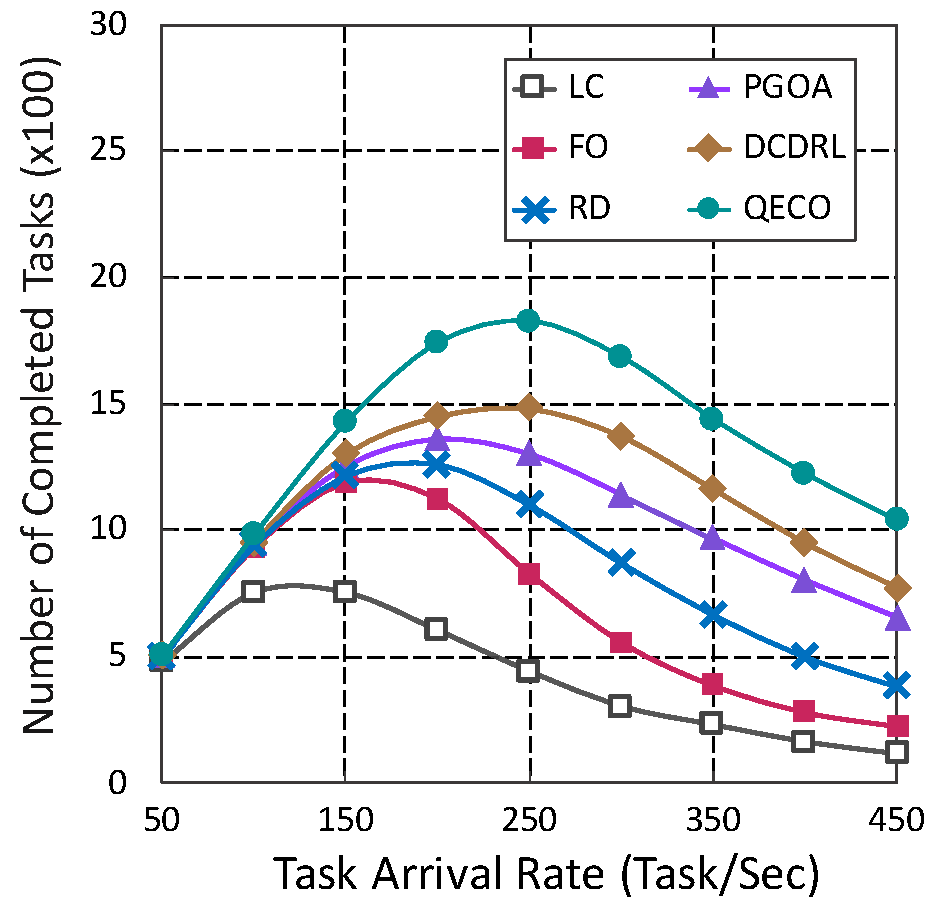
\includegraphics[width=\textwidth]{ drop_1} 
		\textcolor{white}{i}\hspace{0.6cm}(a)
	\end{minipage}
	\hspace{-0.2cm}
	\begin{minipage}[b]{0.3\linewidth}
		\centering
		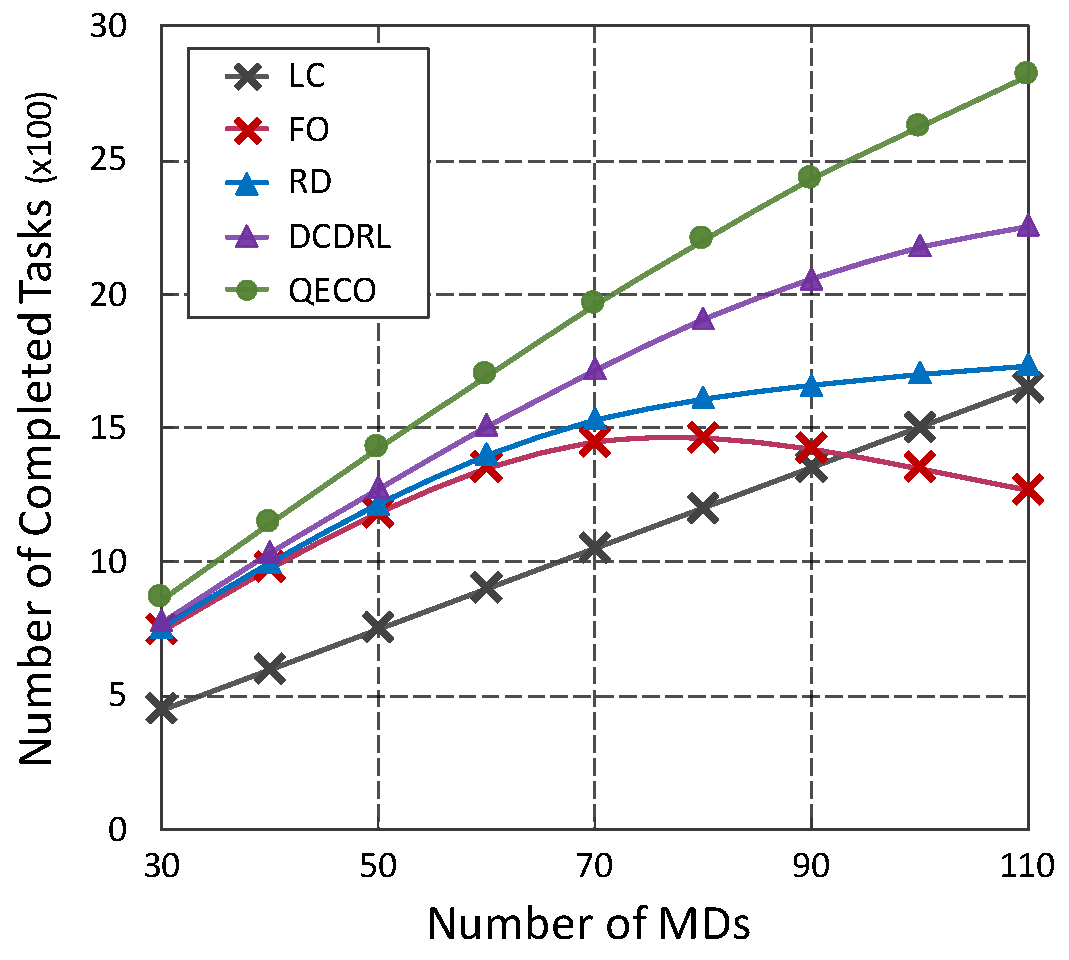
\includegraphics[width=\textwidth]{ drop_2}
		\textcolor{white}{i}\hspace{0.6cm}(b)
	\end{minipage}
	\caption{\textcolor{blue}{The number of completed tasks under different computation workloads: (a) task arrival rate; (b) the number of MDs.}}
	\label{chart1}
\end{figure}\vspace{-8mm}
\begin{figure}[H]\centering
	\captionsetup{name=Fig.}
	\begin{minipage}[b]{0.3\linewidth}
		\centering
		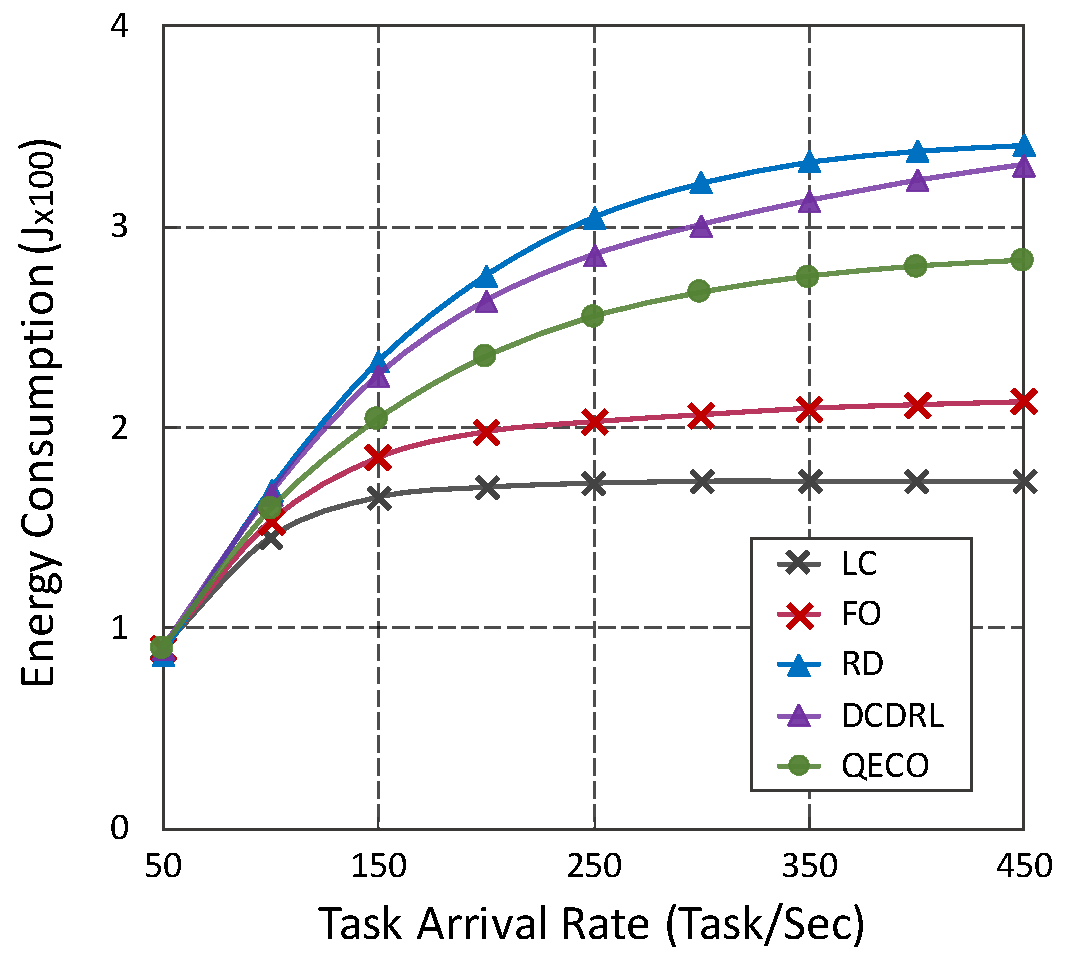
\includegraphics[width=\textwidth]{ energy_1} 		
		\textcolor{white}{i}\hspace{0.6cm}(a)
	\end{minipage}
	\hspace{-0.2cm}
	\begin{minipage}[b]{0.3\linewidth}
		\centering
		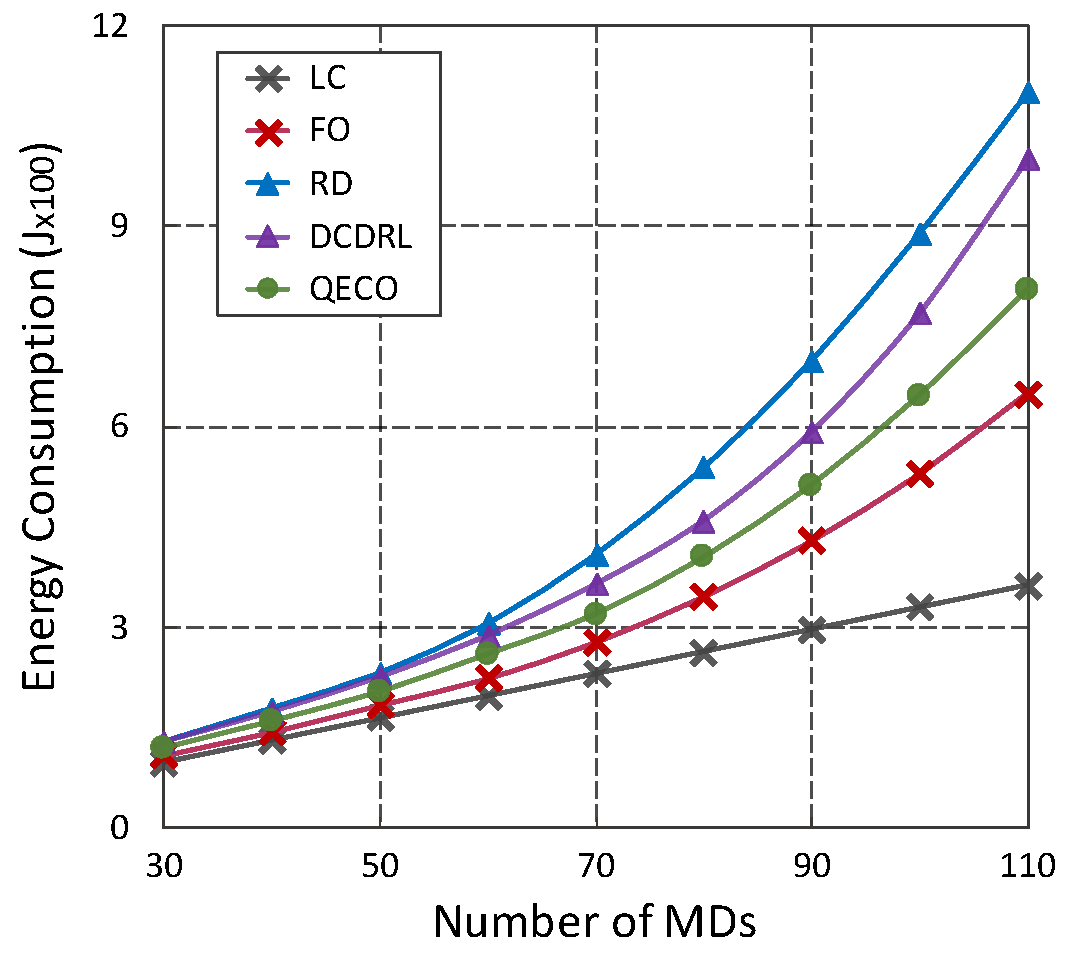
\includegraphics[width=\textwidth]{ energy_2}
		\textcolor{white}{i}\hspace{0.6cm}(b)
	\end{minipage}
	
	\caption{\textcolor{blue}{The overall energy consumption under different computation workloads: (a) task arrival rate; (b) the number of MDs.}}
	\label{chart2}
\end{figure}\vspace{-8mm}
\begin{figure}[H]\centering
	\captionsetup{name=Fig.}
	\begin{minipage}[b]{0.3\linewidth}
		\centering
		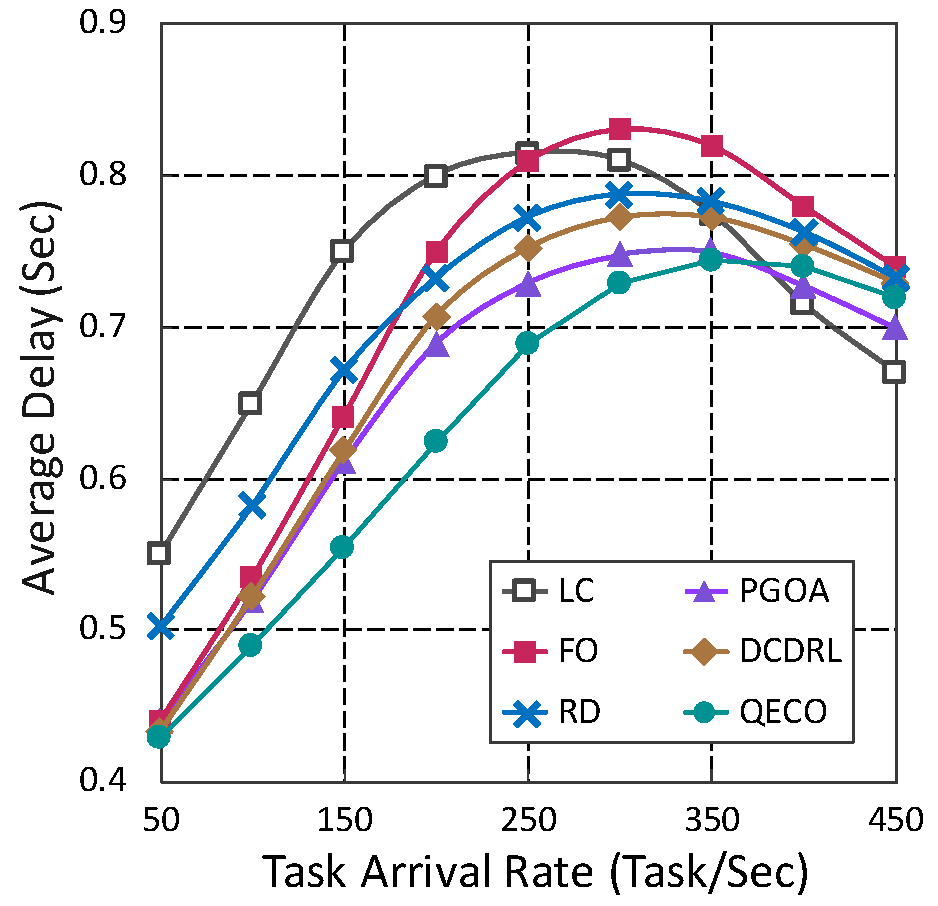
\includegraphics[width=\textwidth]{ delay_1} 		
		\textcolor{white}{i}\hspace{0.6cm}(a)
	\end{minipage}
	\hspace{-0.2cm}
	\begin{minipage}[b]{0.3\linewidth}
		\centering
		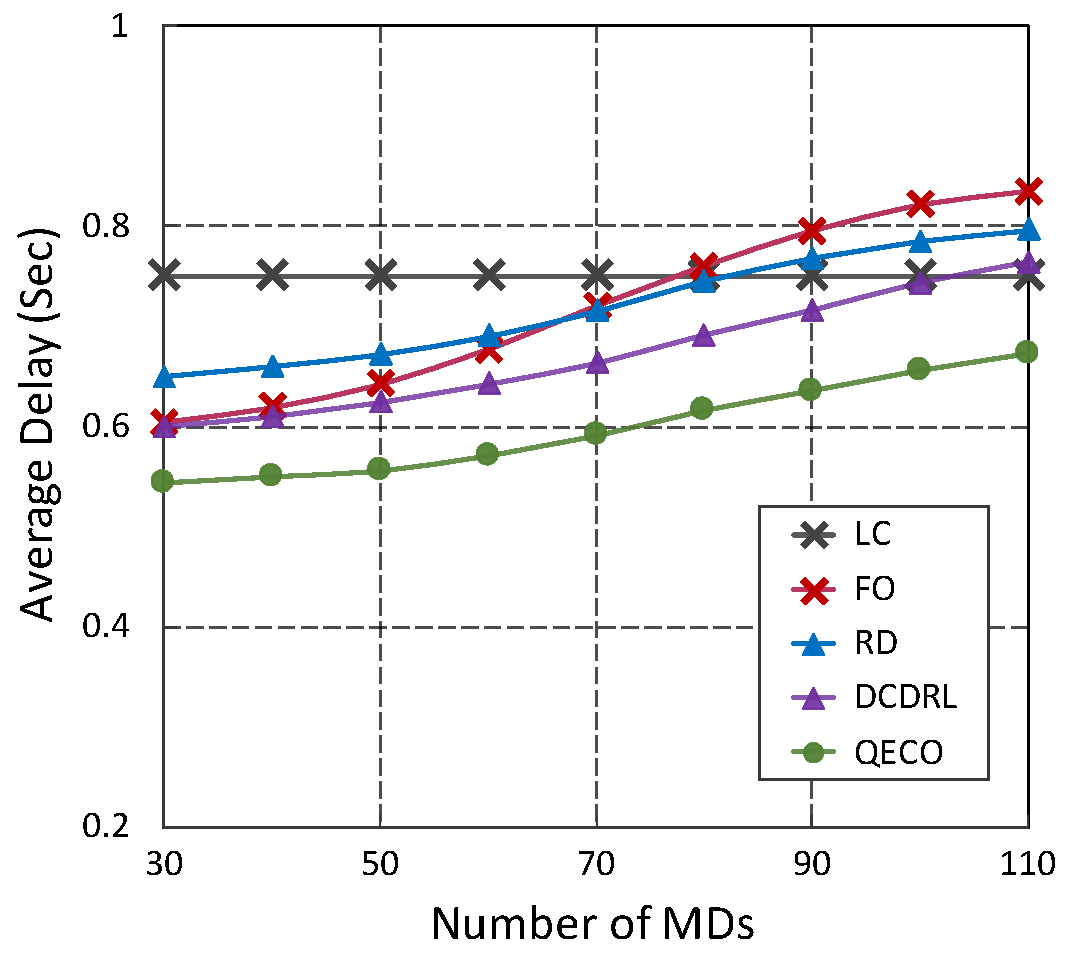
\includegraphics[width=\textwidth]{ delay_2}
		\textcolor{white}{i}\hspace{0.6cm}(b)
	\end{minipage}
	
	\caption{\textcolor{blue}{The average delay under different computation workloads: (a) task arrival rate; (b) the number of MDs.}}
	\label{chart3}
\end{figure} \vspace{-8mm}
\begin{figure}[H]\centering
	\captionsetup{name=Fig.}
	\begin{minipage}[b]{0.3\linewidth}
		\centering
		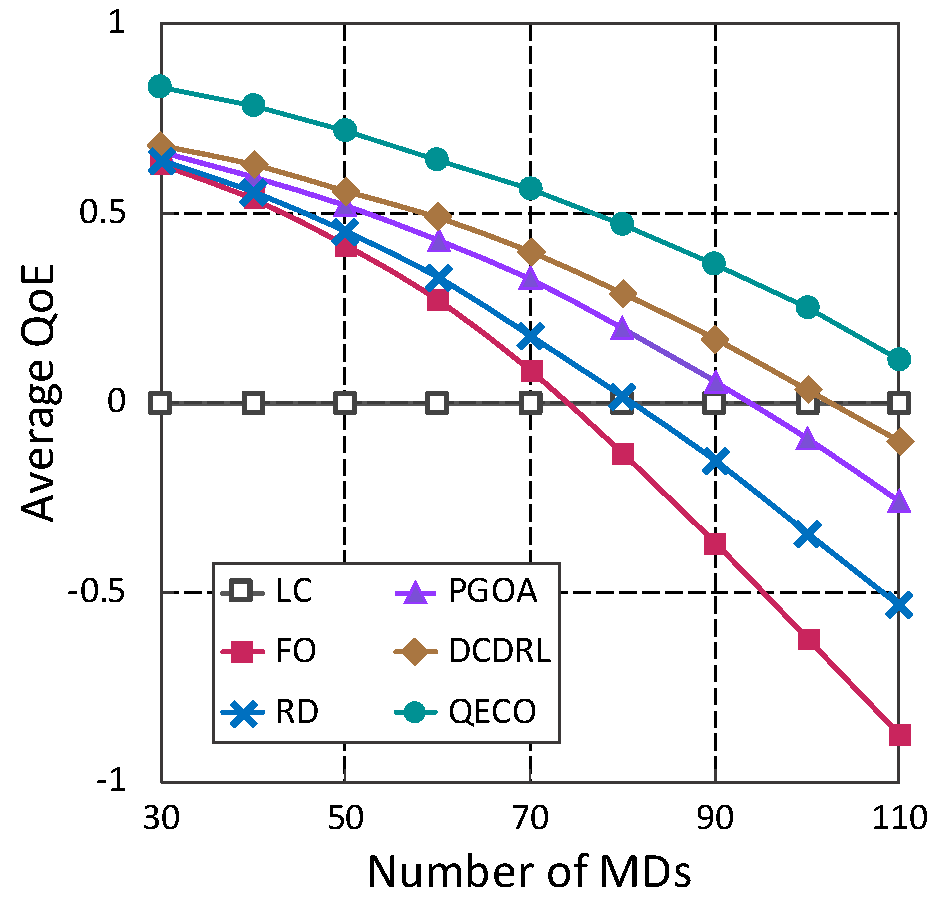
\includegraphics[width=\textwidth]{ qoe_2} 		
		\textcolor{white}{i}\hspace{0.6cm}(a)
	\end{minipage}
	\hspace{-0.2cm}
	\begin{minipage}[b]{0.3\linewidth}
		\centering
		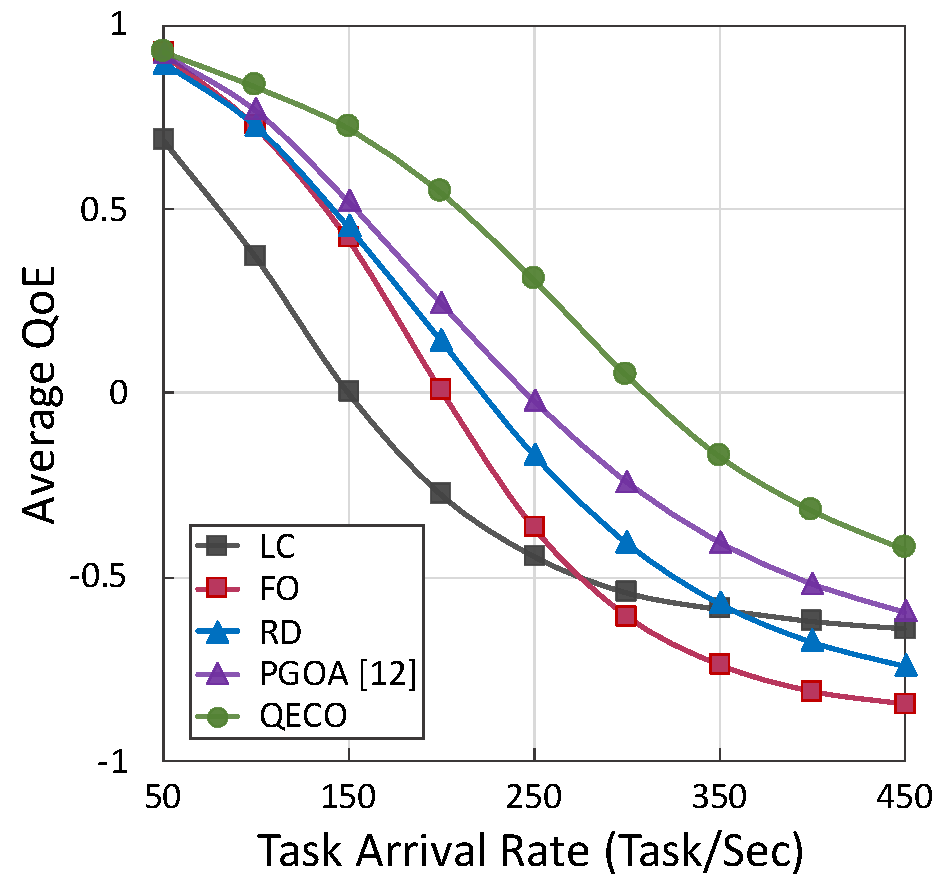
\includegraphics[width=\textwidth]{ qoe_1}
		\textcolor{white}{i}\hspace{0.6cm}(b)
	\end{minipage}
	
	\caption{\textcolor{blue}{The average QoE under different computation workloads: (a) task arrival rate; (b) the number of MDs.}}
	\label{chart44}
\end{figure} 

Furthermore, to enhance the evaluation of our work, we have extended the performance analysis by comparing QECO with two baseline schemes, vanilla DQN and DDQN \cite{van2016deep}. This comparison illustrates the impacts of the LSTM network and dueling architecture. We have added Fig. 7 to Section VI of the revised manuscript.

\begin{figure}[H]
	\captionsetup{name=Fig.}
	\centering
	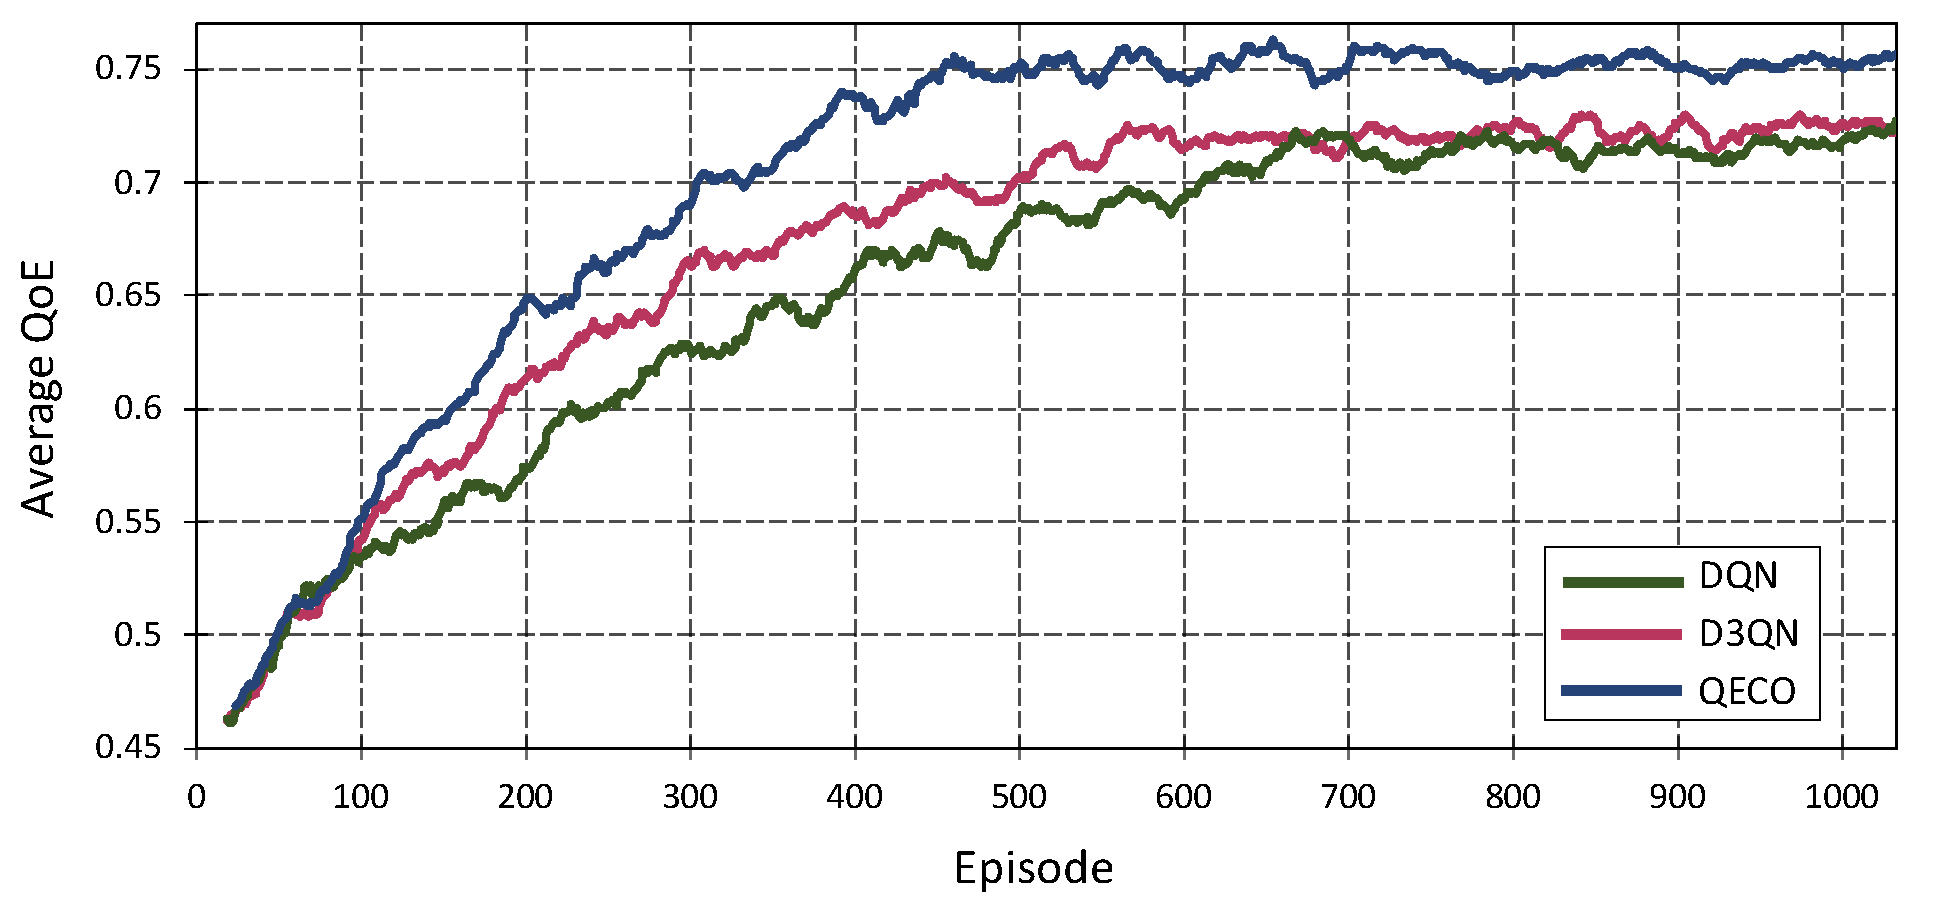
\includegraphics[width=.6\linewidth]{m1}
	\vspace*{-3mm}
	\caption{\textcolor{blue}{The convergence of the average QoE across episodes under different DQN-based methods.}}
	\vspace*{-3mm}
	\label{chart111}
\end{figure}
\begin{my}{1cm}{1cm}
	\rev{
		{\ 
			
			\dots 
			
			
			\,\,\,\,We finally delve into the investigation of the convergence performance of the QECO algorithm in Fig.~\ref{chart111} and Fig. 8. To validate the effectiveness of the QECO algorithm, we assess its convergence rate compared to the vanilla DQN and DDQN configurations \cite{van2016deep}, measured by the average QoE across episodes. As shown in Fig.~\ref{chart111}, as the episodes progress, the MD's network learns efficient policies, ultimately stabilizing as it approaches convergence. Specifically, the DQN, DDQN, and our proposed QECO algorithm converge after approximately 650, 550, and 450 iterations, respectively. The QECO algorithm demonstrates the faster convergence while achieves a higher average QoE than the other methods. underscore the beneficial impact of workload prediction by the LSTM network and highlight its effectiveness in efficiently utilizing the processing capabilities of  MDs and ENs. \\\dots }}
	
\end{my}

\vspace{6mm}




	\item \underline{Reviewer's Comment}: 
	\textit{``I think more explanations should be added for the QoE function. How can the defined function reflect QoE?''} \newline
	
	\underline{Authors' Reply}: Given the importance of evaluating an agent's action in DRL-based computation offloading approaches, we define the QoE maximization problem by considering several key performance factors. QoE is a time-varying performance measure that reflects user satisfaction and is influenced by more than just delay or energy consumption. On the other hand, investigating the trade-off between delay and energy consumption may not adequately address user demands and meet QoE requirements. To capture the agent’s personalized QoE needs, we designed an adaptive trade-off between task completion and cost reduction. In this model, the associated cost is a weighted sum of delay and energy consumption, with the weights dynamically adjusted based on the MD's preferences.\vspace{2mm}
	
	To address the reviewer's comments, we have further explained the QoE function and revised Section IV as follows.
	
	
	
			\begin{my}{1cm}{1cm}
		\rev{
			{\ 
				
				\dots 
				
\,\,\,\,The QoE function reflects user satisfaction with task computation, whether using local or edge resources. QoE accounts for task completion rate, processing delay, and energy consumption. Each user may have unique QoE requirements~\cite{wang2017qoe}. Therefore, we define a multi-dimensional, adaptive structure to assess QoE, balancing these factors according to the MDs preferences, such as prioritizing reduced task delays or energy savings, which may vary over time~\cite{wang2019intelligent},~\cite{mehrabi2019energy}. To capture personalized QoE requirements, we define QoE as a weighted sum of the above factors. Each MD dynamically adjusts these weights to reflect the importance of different factors based on its energy modes, which are performance, power-saving, and ultra-power-saving modes. We now calculate task delay and energy consumption and then introduce the associated cost and QoE function.
								
				\dots
								
				To define associated cost, we use a weighted sum of task delay $\mathcal{D}_i(\boldsymbol{s}_i(t),\boldsymbol{a}_i(t))$ and energy consumption $\mathcal{E}_i(\boldsymbol{s}_i(t),\boldsymbol{a}_i(t))$, where the MD dynamically adjusts the weights based on its energy level to reflect the preference for each factor. \\\dots
}}
	\end{my}




\begin{my}{1cm}{1cm}
	\rev{
		{\small
			\noindent\hspace{-0.5mm}\cite{wang2017qoe} Wang, Ying and Zhou, Wen'an and Zhang, Ping ``QoE Management in Wireless Networks,'' \textit{Springer}, pp. 1085--1101, May 2021.\\[10pt]
			\cite{wang2019intelligent} Wang, Fangxin and Zhang, Cong and Liu, Jiangchuan and Zhu, Yifei and Pang, Haitian and Sun, Lifeng, ``Intelligent edge-assisted crowdcast with deep reinforcement learning for personalized QoE,'' in \textit{IEEE INFOCOM 2019-IEEE Conference on Computer Communications}, pp. 910--918, May 2019.\\[10pt]
			\cite{mehrabi2019energy} Mehrabi, Abbas and Siekkinen, Matti and Yl{\"a}-J{\"a}{\"a}ski, Antti, ``Energy-aware QoE and backhaul traffic optimization in green edge adaptive mobile video streaming,'' \textit{ IEEE trans. green commun. netw.}, vol. 3, no. 3, pp. 828--839, Sep 2019.}\\}
\end{my}\vspace{6mm}

We have also revised the explanation related to Fig. 6 and Fig. 7 in Section VI of the revised manuscript to further specify how the QECO algorithm improves QoE of users. The following paragraph shows the changes we have made in Section VI of the revised manuscript.
		\begin{my}{1cm}{1cm}
	\rev{
		{\ 
			
			\dots \color{black}
			
			\,\,\,\,We further investigate the overall improvement achieved by the QECO algorithm in comparison to other methods in terms of the average QoE. This metric signifies the advantages MDs obtain by utilizing different algorithms. \textcolor{blue}{Fig. 6 (a) shows the average QoE for different values of the task arrival rate. This figure highlights the superiority of the QECO algorithm in providing MDs with an enhanced experience. At lower task arrival rates (i.e., 50-150), QECO performs optimally and maintains an average QoE of at least 0.72, while the other methods experience a steeper decline, with average QoE dropping to 0--0.56. Specifically, at a task arrival rate of 200, QECO improves the average QoE by at least 65.7\% compared to other methods in the positive average QoE range. As task arrival rates increase to 300, the average QoE significantly decreases for all methods due to increased competition for resources in the MEC system. However, QECO still maintains a positive average QoE, while other methods fall to negative values, with a decline of up to -0.17. For higher task arrival rates (i.e., 350–450), QECO experiences a negative average QoE, but it shows at least a 42.6\%, 28.5\%, and 22.6\% smaller reduction in average QoE compared to RD, PGOA, and DCDRL, respectively.} \vspace{3mm}
			
			
			
			\,\,\,\, Fig. 6 (b) illustrates the average QoE when we increase the number of MDs. The EN's workload grows when there are a larger number of MDs, leading to a reduction in the average QoE of all methods except LC. However, QECO effectively manages the uncertain load at the ENs. \textcolor{blue}{When the number of MDs increases from 30 to 110, QECO consistently maintains at least a 24.8\% higher QoE compared to the other methods. Specifically, at a moderate number of 70 MDs, QECO achieves an average QoE of 0.57, showing a 70.3\% and 44.7\% improvement compared to PGOA and DCDRL, respectively.} It is worth noting that although improvements in each of the QoE factors can contribute to enhancing system performance, it is essential to consider the user's demands in each time slot. Therefore, the key difference between QECO and other methods is that it prioritizes users' demands, enabling it to strike an appropriate balance among them, ultimately leading to a higher QoE for MDs.
			\vspace{3mm}\\\dots }}
	
\end{my}\vspace{6mm}
	


	\item \underline{Reviewer's Comment}: 
	\textit{``(a) What are inputs and outputs of Algorithm 2? (b) They should be added to make readers clearly understand the results.''} \\\newline
	\underline{Authors' Reply}: (a) To address the reviewer comment, we have revised the relevant paragraph of Section V to clarify the inputs and outputs of Algorithms 2.\newline
	
	\begin{my}{1cm}{1cm} 
		\rev{
		
		\dots \color{black}
		
		
		In particular, regarding experience $n$, the target-Q value $\hat{Q}_{i,n}^{\text{T}}$ represents the long-term QoE for action $\boldsymbol{a}_i(n)$ under state $\boldsymbol{s}_i(n)$. This value corresponds to the QoE observed in experience $n$, as well as the approximate expected upcoming QoE. 
			\textcolor{blue}{Based on the set $\mathcal{N}$, the EN computes the vector $\hat{\mathbf{Q}}_i^{\text{T}} = (\hat{Q}^{\text{T}}_{i,n})_{n \in \mathcal{N}}$ and trains the MD's neural network (steps 11-21 of Algorithm~\ref{alg:cap2}) to update the parameter vector $\theta^{\text{E}}_i$ in $\textit{Net}_i^{\text{E}}$ for the next MD's \textit{UpdateRequest}.} The key idea of updating $\textit{Net}_i^{\text{E}}$ is to minimize the disparity in Q-values between $\textit{Net}_i^{\text{E}}$ and $\textit{Net}_i^{\text{T}}$, as indicated by the following loss function:
			
			\dots}
	\end{my}
		
	We have also revised Algorithms 1 and 2 and included the list of inputs and outputs.\\	
	

\begin{my}{0.5cm}{0.5cm}	
\rev{\begin{minipage}[b]{0.87\textwidth} 
	\begin{algorithm}[H] \caption{Offloading Decision Algorithm at MD $i \in \mathcal{I}$}\label{alg:cap2} \centering 
		\begin{algorithmic}[1] \renewcommand{\algorithmicrequire}{\textbf{\textcolor{blue}{Input:}}} \renewcommand{\algorithmicensure}{\textbf{\textcolor{blue}{Output:}}} \Require \textcolor{blue}{experience $(\boldsymbol{s}_i(t), \boldsymbol{a}_i(t), \boldsymbol{q}_i(t), \boldsymbol{s}_i(t+1))$ from MD $i \in \mathcal{I}$} \Ensure \textcolor{blue}{parameter vector $\theta_i^{\text{E}}$} 
	\end{algorithmic} 
\end{algorithm} 
\end{minipage}
\vspace{5mm}

\begin{minipage}[b]{0.87\textwidth} 
	\begin{algorithm}[H] \caption{Training Process Algorithm at EN $j \in \mathcal{J}$}\label{alg:cap2} \centering 
		\begin{algorithmic}[1] \renewcommand{\algorithmicrequire}{\textbf{Input:}} \renewcommand{\algorithmicensure}{\textbf{Output:}}\Require state space $\mathcal{S}$, action space $\mathcal{A}$
			\Ensure MD $i \in \mathcal{I}$ experience  \textcolor{blue}{ $(\hspace{-0.2mm}\boldsymbol{s}_i(\hspace{-0.2mm}t\hspace{-0.2mm}), \boldsymbol{a}_i(\hspace{-0.2mm}t\hspace{-0.2mm}), \boldsymbol{q}_i(\hspace{-0.2mm}t\hspace{-0.2mm}), \boldsymbol{s}_i(\hspace{-0.2mm}t\hspace{-0.3mm}+\hspace{-0.3mm}\hspace{-0.2mm}1\hspace{-0.2mm}\hspace{-0.2mm})\hspace{-0.2mm})$}
		\end{algorithmic} 
	\end{algorithm} 
\end{minipage}}
\end{my}
	

\vspace{10mm}
	\item \underline{Reviewer's Comment}: 
	\textit{``The authors should open their experiments in github, so that other researchers can compare their work with other ones.''} \newline
	\underline{Authors' Reply}: To address the reviewer comment, we have made our GitHub repository  publicly available. It has also been introduced and cited in metadata and Section VI as follows.
	
	\begin{my}{1cm}{1cm}
		\rev{
			
			\dots
			
			\,\,\,\, \textcolor{blue}{The algorithm's source code is available at \cite{QECO}}

	}
	\end{my} \vspace{6mm}




	\item \underline{Reviewer's Comment}: 
	\textit{``The following references closely related to the current work should be discussed or compared with the current work for completeness.''} \newline
		\begin{my}{1cm}{1cm}
		\rev{
			{\small
				\noindent\hspace{-0.5mm}\cite{wu2023computation} G. Wu, H. Wang, H. Zhang, Y. Zhao, S. Yu, and S. Shen, ``Computation offloading method using stochastic games for software-defined-network-based multiagent mobile edge computing,'' \textit{IEEE Internet of Things Journal}, vol. 10, no. 20, pp. 17620–17634, Oct. 2023.\\[6pt]
				\cite{wu2024privacy} G. Wu, X. Chen, Z. Gao, H. Zhang, S. Yu, and S. Shen, ``Privacy-preserving offloading scheme in multi-access mobile edge computing based on MADRL,'' \textit{Journal of Parallel and Distributed Computing}, vol. 10, no. 1, pp. 451--460, Mar. 2022.\\[6pt]
				\cite{wu2024combining}  G. Wu, X. Chen, Y. Shen, Z. Xu, H. Zhang, S. Shen, and S. Yu,``Combining Lyapunov optimization with Actor-Critic networks for privacy-aware IIoT computation offloading,'' in \textit{IEEE Internet of Things Journal}, 2024, Early Access\\[6pt]
				\cite{wu2023multi} G. Wu, Z. Xu, H. Zhang, S. Shen, and S. Yu,  ``Multi-agent DRL for joint completion delay and energy consumption with queuing theory in MEC-based IIoT,'' in \textit{Journal of Parallel and Distributed Computing}, vol. 176, pp. 80–94, Jun. 2023\\[6pt]}\\}
	\end{my}

	\underline{Authors' Reply}: In response to the reviewer's comment, we have cited these works in the newly added related work section (i.e., Section II) and discussed their strengths and limitations. The following sentences reflect the changes we made in Section II of the revised manuscript. \vspace{5mm}
	
	\begin{my}{1cm}{1cm}
		\rev{
			{
				\color{black}
				
				
				
				\dots
				
				\,\,\,\,
				In MEC environments, multiple objectives often compete, requiring a balance in decision-making. For instance, task offloading must carefully navigate trade-offs between delay and energy consumption, as well as balance energy usage against the number of completed tasks. Research has increasingly addressed these multi-objective optimization challenges.
				 \textcolor{blue}{\dots
				To optimize privacy protection and quality of service, authors in \cite{wu2024privacy} investigated the joint computation offloading and power allocation problems for the IIoT network. They modeled the problem as an MDP and proposed a multi-agent DQN-based algorithm. 
				\dots
				Wu \textit{et al.} in \cite{wu2023computation} introduced a stochastic game-based resource allocation in the SDN-based MEC network. They used an MDP and proposed a multi-agent RL method to minimize both energy consumption and processing delay. }
				
				\dots
				
				\,\,\,\,
				To further enhance the modeling of real-world scenarios, some studies have applied queuing theory to model MEC systems, which helps capture the dynamic nature of the network and allows MEC systems to allocate computational and transmission resources more efficiently.
				\textcolor{blue}{\dots
				To address the privacy-aware computation offloading problem, Wu \textit{et al.} in \cite{wu2024combining} modeled the problem as an MDP and proposed a DQN-based method to optimize the computation rate and energy consumption in a queuing-based IIoT network. \dots
				Wu \textit{et al.} in \cite{wu2023multi} investigated the computation offloading problem in a queuing-based MEC IIoT system. They modeled the problem as a POMDP and proposed a multi-agent proximal policy optimization (PPO)-based method to obtain the optimal offloading strategy in dynamic environments.
				\dots}

				
				\dots
				
				
		}}
	\end{my}\vspace{6mm}

We have provided a survey of the recently published state-of-the-art works in Section II of the revised manuscript, as mentioned in our response to Reviewer's Comment 1.\newline


	
\end{enumerate}

\vspace{10mm}

\textit{We would like to gratefully thank the reviewer for the valuable comments and suggestions. We hope that we have satisfactorily addressed these comments.}\newline



\end{document}


